\documentclass[twoside]{book}

% Packages required by doxygen
\usepackage{calc}
\usepackage{doxygen}
\usepackage{graphicx}
\usepackage[utf8]{inputenc}
\usepackage{makeidx}
\usepackage{multicol}
\usepackage{multirow}
\usepackage{textcomp}
\usepackage[table]{xcolor}

% Font selection
\usepackage[T1]{fontenc}
\usepackage{mathptmx}
\usepackage[scaled=.90]{helvet}
\usepackage{courier}
\usepackage{amssymb}
\usepackage{sectsty}
\renewcommand{\familydefault}{\sfdefault}
\allsectionsfont{%
  \fontseries{bc}\selectfont%
  \color{darkgray}%
}
\renewcommand{\DoxyLabelFont}{%
  \fontseries{bc}\selectfont%
  \color{darkgray}%
}

% Page & text layout
\usepackage{geometry}
\geometry{%
  a4paper,%
  top=2.5cm,%
  bottom=2.5cm,%
  left=2.5cm,%
  right=2.5cm%
}
\tolerance=750
\hfuzz=15pt
\hbadness=750
\setlength{\emergencystretch}{15pt}
\setlength{\parindent}{0cm}
\setlength{\parskip}{0.2cm}
\makeatletter
\renewcommand{\paragraph}{%
  \@startsection{paragraph}{4}{0ex}{-1.0ex}{1.0ex}{%
    \normalfont\normalsize\bfseries\SS@parafont%
  }%
}
\renewcommand{\subparagraph}{%
  \@startsection{subparagraph}{5}{0ex}{-1.0ex}{1.0ex}{%
    \normalfont\normalsize\bfseries\SS@subparafont%
  }%
}
\makeatother

% Headers & footers
\usepackage{fancyhdr}
\pagestyle{fancyplain}
\fancyhead[LE]{\fancyplain{}{\bfseries\thepage}}
\fancyhead[CE]{\fancyplain{}{}}
\fancyhead[RE]{\fancyplain{}{\bfseries\leftmark}}
\fancyhead[LO]{\fancyplain{}{\bfseries\rightmark}}
\fancyhead[CO]{\fancyplain{}{}}
\fancyhead[RO]{\fancyplain{}{\bfseries\thepage}}
\fancyfoot[LE]{\fancyplain{}{}}
\fancyfoot[CE]{\fancyplain{}{}}
\fancyfoot[RE]{\fancyplain{}{\bfseries\scriptsize Generated on Thu Dec 17 2015 18\-:58\-:59 for E\-Marche by Doxygen }}
\fancyfoot[LO]{\fancyplain{}{\bfseries\scriptsize Generated on Thu Dec 17 2015 18\-:58\-:59 for E\-Marche by Doxygen }}
\fancyfoot[CO]{\fancyplain{}{}}
\fancyfoot[RO]{\fancyplain{}{}}
\renewcommand{\footrulewidth}{0.4pt}
\renewcommand{\chaptermark}[1]{%
  \markboth{#1}{}%
}
\renewcommand{\sectionmark}[1]{%
  \markright{\thesection\ #1}%
}

% Indices & bibliography
\usepackage{natbib}
\usepackage[titles]{tocloft}
\setcounter{tocdepth}{3}
\setcounter{secnumdepth}{5}
\makeindex

% Custom commands
\newcommand{\clearemptydoublepage}{%
  \newpage{\pagestyle{empty}\cleardoublepage}%
}


%===== C O N T E N T S =====

\begin{document}

% Titlepage & ToC
\pagenumbering{roman}
\begin{titlepage}
\vspace*{7cm}
\begin{center}%
{\Large E\-Marche }\\
\vspace*{1cm}
{\large Generated by Doxygen 1.8.6}\\
\vspace*{0.5cm}
{\small Thu Dec 17 2015 18:58:59}\\
\end{center}
\end{titlepage}
\clearemptydoublepage
\tableofcontents
\clearemptydoublepage
\pagenumbering{arabic}

%--- Begin generated contents ---
\chapter{Hierarchical Index}
\section{Hiérarchie des classes}
Cette liste d'héritage est classée approximativement par ordre alphabétique \-:\begin{DoxyCompactList}
\item \contentsline{section}{Avis}{\pageref{class_avis}}{}
\item \contentsline{section}{Categorie}{\pageref{class_categorie}}{}
\item \contentsline{section}{Coords\-Bancaires}{\pageref{class_coords_bancaires}}{}
\item \contentsline{section}{Etat\-Connexion}{\pageref{class_etat_connexion}}{}
\begin{DoxyCompactList}
\item \contentsline{section}{Etat\-Connecte}{\pageref{class_etat_connecte}}{}
\item \contentsline{section}{Etat\-Deconnecte}{\pageref{class_etat_deconnecte}}{}
\end{DoxyCompactList}
\item \contentsline{section}{Etat\-Vente}{\pageref{class_etat_vente}}{}
\begin{DoxyCompactList}
\item \contentsline{section}{Vente\-Enchere}{\pageref{class_vente_enchere}}{}
\item \contentsline{section}{Vente\-Normale}{\pageref{class_vente_normale}}{}
\end{DoxyCompactList}
\item \contentsline{section}{Gestion\-Bdd}{\pageref{class_gestion_bdd}}{}
\item \contentsline{section}{Les\-Produits}{\pageref{class_les_produits}}{}
\item \contentsline{section}{Les\-Utilisateurs}{\pageref{class_les_utilisateurs}}{}
\item \contentsline{section}{Produit}{\pageref{class_produit}}{}
\item Q\-Dialog\begin{DoxyCompactList}
\item \contentsline{section}{Dialog\-Acheter}{\pageref{class_dialog_acheter}}{}
\item \contentsline{section}{Dialog\-Ajouter\-Vente}{\pageref{class_dialog_ajouter_vente}}{}
\item \contentsline{section}{Dialog\-Connexion}{\pageref{class_dialog_connexion}}{}
\end{DoxyCompactList}
\item Q\-Widget\begin{DoxyCompactList}
\item \contentsline{section}{Ma\-Fenetre}{\pageref{class_ma_fenetre}}{}
\end{DoxyCompactList}
\item \contentsline{section}{Ui\-\_\-\-Dialog\-Acheter}{\pageref{class_ui___dialog_acheter}}{}
\begin{DoxyCompactList}
\item \contentsline{section}{Ui\-:\-:Dialog\-Acheter}{\pageref{class_ui_1_1_dialog_acheter}}{}
\end{DoxyCompactList}
\item \contentsline{section}{Ui\-\_\-\-Dialog\-Ajouter\-Vente}{\pageref{class_ui___dialog_ajouter_vente}}{}
\begin{DoxyCompactList}
\item \contentsline{section}{Ui\-:\-:Dialog\-Ajouter\-Vente}{\pageref{class_ui_1_1_dialog_ajouter_vente}}{}
\end{DoxyCompactList}
\item \contentsline{section}{Ui\-\_\-\-Dialog\-Connexion}{\pageref{class_ui___dialog_connexion}}{}
\begin{DoxyCompactList}
\item \contentsline{section}{Ui\-:\-:Dialog\-Connexion}{\pageref{class_ui_1_1_dialog_connexion}}{}
\end{DoxyCompactList}
\item \contentsline{section}{Ui\-\_\-\-Dialog\-Inscription}{\pageref{class_ui___dialog_inscription}}{}
\begin{DoxyCompactList}
\item \contentsline{section}{Ui\-:\-:Dialog\-Inscription}{\pageref{class_ui_1_1_dialog_inscription}}{}
\end{DoxyCompactList}
\item \contentsline{section}{Ui\-\_\-\-Dialog\-Modification\-Profil}{\pageref{class_ui___dialog_modification_profil}}{}
\begin{DoxyCompactList}
\item \contentsline{section}{Ui\-:\-:Dialog\-Modification\-Profil}{\pageref{class_ui_1_1_dialog_modification_profil}}{}
\end{DoxyCompactList}
\item \contentsline{section}{Utilisateur}{\pageref{class_utilisateur}}{}
\item \contentsline{section}{Vue}{\pageref{class_vue}}{}
\begin{DoxyCompactList}
\item \contentsline{section}{Ma\-Fenetre}{\pageref{class_ma_fenetre}}{}
\end{DoxyCompactList}
\end{DoxyCompactList}

\chapter{Class Index}
\section{Liste des classes}
Liste des classes, structures, unions et interfaces avec une brève description \-:\begin{DoxyCompactList}
\item\contentsline{section}{\hyperlink{class_avis}{Avis} \\*
\begin{DoxyItemize}
\item Représente un avis donné par un utilisateur sur un autre utilisateur ou un produit, avec un commentaire et une note 
\end{DoxyItemize}}{\pageref{class_avis}}{}
\item\contentsline{section}{\hyperlink{class_categorie}{Categorie} \\*
\begin{DoxyItemize}
\item Représente une catégorie de produits 
\end{DoxyItemize}}{\pageref{class_categorie}}{}
\item\contentsline{section}{\hyperlink{class_coords_bancaires}{Coords\-Bancaires} \\*Cette classe contient les données bancaires d'un utilisateur }{\pageref{class_coords_bancaires}}{}
\item\contentsline{section}{\hyperlink{class_dialog_ajouter_vente}{Dialog\-Ajouter\-Vente} \\*
\begin{DoxyItemize}
\item Boîte de dialoque permettant l'ajout d'un produit en vente 
\end{DoxyItemize}}{\pageref{class_dialog_ajouter_vente}}{}
\item\contentsline{section}{\hyperlink{class_dialog_connexion}{Dialog\-Connexion} \\*
\begin{DoxyItemize}
\item Boîte de dialogue permettant de se connecter 
\end{DoxyItemize}}{\pageref{class_dialog_connexion}}{}
\item\contentsline{section}{\hyperlink{class_dialog_inscription}{Dialog\-Inscription} \\*
\begin{DoxyItemize}
\item Boîte de dialogue permettant d'inscrire un nouvel utilisateur 
\end{DoxyItemize}}{\pageref{class_dialog_inscription}}{}
\item\contentsline{section}{\hyperlink{class_dialog_modification_profil}{Dialog\-Modification\-Profil} \\*
\begin{DoxyItemize}
\item Boîte de dialogue permettant de modifier les données du profil utilisateur 
\end{DoxyItemize}}{\pageref{class_dialog_modification_profil}}{}
\item\contentsline{section}{\hyperlink{class_etat_connecte}{Etat\-Connecte} \\*Cette classe gère les utilisateurs connectés }{\pageref{class_etat_connecte}}{}
\item\contentsline{section}{\hyperlink{class_etat_connexion}{Etat\-Connexion} \\*Cette classe gère les états de connexion d'un utilisateur (connecté ou déconnecté) }{\pageref{class_etat_connexion}}{}
\item\contentsline{section}{\hyperlink{class_etat_deconnecte}{Etat\-Deconnecte} \\*Cette classe gère les utilisateurs déconnectés }{\pageref{class_etat_deconnecte}}{}
\item\contentsline{section}{\hyperlink{class_etat_vente}{Etat\-Vente} \\*Cette classe gère l'état d'une vente (enchère ou normale) }{\pageref{class_etat_vente}}{}
\item\contentsline{section}{\hyperlink{class_gestion_bdd}{Gestion\-Bdd} \\*
\begin{DoxyItemize}
\item Gère le stockage des utilisateurs, des produits, et la mise à jour des vues 
\end{DoxyItemize}}{\pageref{class_gestion_bdd}}{}
\item\contentsline{section}{\hyperlink{class_les_produits}{Les\-Produits} \\*Cette classe gère la liste des produits }{\pageref{class_les_produits}}{}
\item\contentsline{section}{\hyperlink{class_les_utilisateurs}{Les\-Utilisateurs} \\*
\begin{DoxyItemize}
\item Gère un vector de pointeurs vers des utilisateurs 
\end{DoxyItemize}}{\pageref{class_les_utilisateurs}}{}
\item\contentsline{section}{\hyperlink{class_ma_fenetre}{Ma\-Fenetre} \\*
\begin{DoxyItemize}
\item Affichage principal de l'application 
\end{DoxyItemize}}{\pageref{class_ma_fenetre}}{}
\item\contentsline{section}{\hyperlink{class_produit}{Produit} \\*Cette classe gère le stockage d'un produit }{\pageref{class_produit}}{}
\item\contentsline{section}{\hyperlink{class_utilisateur}{Utilisateur} \\*
\begin{DoxyItemize}
\item Contient toutes les informations personnelles d'un utilisateur 
\end{DoxyItemize}}{\pageref{class_utilisateur}}{}
\item\contentsline{section}{\hyperlink{class_vente_enchere}{Vente\-Enchere} \\*Cette classe gère une vente aux enchères }{\pageref{class_vente_enchere}}{}
\item\contentsline{section}{\hyperlink{class_vente_normale}{Vente\-Normale} \\*Cette classe gère une vente normale }{\pageref{class_vente_normale}}{}
\item\contentsline{section}{\hyperlink{class_vue}{Vue} \\*
\begin{DoxyItemize}
\item Permet la mise à jour des vues 
\end{DoxyItemize}}{\pageref{class_vue}}{}
\end{DoxyCompactList}

\chapter{Class Documentation}
\hypertarget{class_avis}{\section{Référence de la classe Avis}
\label{class_avis}\index{Avis@{Avis}}
}


The \hyperlink{class_avis}{Avis} class -\/ Représente un avis donné par un utilisateur sur un autre utilisateur ou un produit, avec un commentaire et une note.  




{\ttfamily \#include $<$Avis.\-h$>$}

\subsection*{Fonctions membres publiques}
\begin{DoxyCompactItemize}
\item 
\hyperlink{class_avis_a93b6b6e8ce6e399a9dc017284063a841}{Avis} (std\-::string author, unsigned int notation)
\begin{DoxyCompactList}\small\item\em \hyperlink{class_avis}{Avis} -\/ Note sans commentaire. \end{DoxyCompactList}\item 
\hyperlink{class_avis_ada1766d4665eded0f8d582b366f56bfe}{Avis} (std\-::string author, unsigned int notation, std\-::string com)
\begin{DoxyCompactList}\small\item\em \hyperlink{class_avis}{Avis} -\/ Note et commentaire. \end{DoxyCompactList}\item 
unsigned int \hyperlink{class_avis_a38aac72b52990bbe4f7bcec663c560c6}{get\-Note} ()
\begin{DoxyCompactList}\small\item\em get\-Note \end{DoxyCompactList}\item 
std\-::string \hyperlink{class_avis_ae03e2b620c88bcc258821b8247529425}{get\-Commentaire} ()
\begin{DoxyCompactList}\small\item\em get\-Commentaire \end{DoxyCompactList}\item 
std\-::string \hyperlink{class_avis_a291d331943b1bcb18ee4290624f5a178}{get\-Auteur} ()
\begin{DoxyCompactList}\small\item\em get\-Auteur \end{DoxyCompactList}\item 
void \hyperlink{class_avis_abbab76777e1327d7f88d20fce541c7a5}{decrit} (std\-::ostream \&os)
\begin{DoxyCompactList}\small\item\em decrit -\/ Ecrit toutes les données de l'avis dans un flux donné en paramètre \end{DoxyCompactList}\item 
std\-::string \hyperlink{class_avis_a517878e3f5196c23cc179f3fe5a1a98d}{decrit} ()
\begin{DoxyCompactList}\small\item\em decrit -\/ convertit un flux en string \end{DoxyCompactList}\item 
void \hyperlink{class_avis_af94b335023000d4ded81528c90e86c32}{affiche} (std\-::ostream \&os)
\begin{DoxyCompactList}\small\item\em affiche -\/ Ecrit toutes les données d'un avis d'un flux vers une sortie \end{DoxyCompactList}\end{DoxyCompactItemize}


\subsection{Description détaillée}
The \hyperlink{class_avis}{Avis} class -\/ Représente un avis donné par un utilisateur sur un autre utilisateur ou un produit, avec un commentaire et une note. 

\subsection{Documentation des constructeurs et destructeur}
\hypertarget{class_avis_a93b6b6e8ce6e399a9dc017284063a841}{\index{Avis@{Avis}!Avis@{Avis}}
\index{Avis@{Avis}!Avis@{Avis}}
\subsubsection[{Avis}]{\setlength{\rightskip}{0pt plus 5cm}Avis\-::\-Avis (
\begin{DoxyParamCaption}
\item[{std\-::string}]{author, }
\item[{unsigned int}]{notation}
\end{DoxyParamCaption}
)\hspace{0.3cm}{\ttfamily [inline]}}}\label{class_avis_a93b6b6e8ce6e399a9dc017284063a841}


\hyperlink{class_avis}{Avis} -\/ Note sans commentaire. 


\begin{DoxyParams}{Paramètres}
{\em author} & -\/ Auteur de l'avis \\
\hline
{\em notation} & -\/ Note donnée \\
\hline
\end{DoxyParams}
\hypertarget{class_avis_ada1766d4665eded0f8d582b366f56bfe}{\index{Avis@{Avis}!Avis@{Avis}}
\index{Avis@{Avis}!Avis@{Avis}}
\subsubsection[{Avis}]{\setlength{\rightskip}{0pt plus 5cm}Avis\-::\-Avis (
\begin{DoxyParamCaption}
\item[{std\-::string}]{author, }
\item[{unsigned int}]{notation, }
\item[{std\-::string}]{com}
\end{DoxyParamCaption}
)\hspace{0.3cm}{\ttfamily [inline]}}}\label{class_avis_ada1766d4665eded0f8d582b366f56bfe}


\hyperlink{class_avis}{Avis} -\/ Note et commentaire. 


\begin{DoxyParams}{Paramètres}
{\em author} & -\/ Auteur de l'avis \\
\hline
{\em notation} & -\/ Note donnée \\
\hline
{\em com} & -\/ Commentaire donné \\
\hline
\end{DoxyParams}


\subsection{Documentation des fonctions membres}
\hypertarget{class_avis_af94b335023000d4ded81528c90e86c32}{\index{Avis@{Avis}!affiche@{affiche}}
\index{affiche@{affiche}!Avis@{Avis}}
\subsubsection[{affiche}]{\setlength{\rightskip}{0pt plus 5cm}void Avis\-::affiche (
\begin{DoxyParamCaption}
\item[{std\-::ostream \&}]{os}
\end{DoxyParamCaption}
)\hspace{0.3cm}{\ttfamily [inline]}}}\label{class_avis_af94b335023000d4ded81528c90e86c32}


affiche -\/ Ecrit toutes les données d'un avis d'un flux vers une sortie 


\begin{DoxyParams}{Paramètres}
{\em os} & -\/ Sortie, par exemple \-: cout \\
\hline
\end{DoxyParams}
\hypertarget{class_avis_abbab76777e1327d7f88d20fce541c7a5}{\index{Avis@{Avis}!decrit@{decrit}}
\index{decrit@{decrit}!Avis@{Avis}}
\subsubsection[{decrit}]{\setlength{\rightskip}{0pt plus 5cm}void Avis\-::decrit (
\begin{DoxyParamCaption}
\item[{std\-::ostream \&}]{os}
\end{DoxyParamCaption}
)\hspace{0.3cm}{\ttfamily [inline]}}}\label{class_avis_abbab76777e1327d7f88d20fce541c7a5}


decrit -\/ Ecrit toutes les données de l'avis dans un flux donné en paramètre 


\begin{DoxyParams}{Paramètres}
{\em os} & -\/ Flux \\
\hline
\end{DoxyParams}
\hypertarget{class_avis_a517878e3f5196c23cc179f3fe5a1a98d}{\index{Avis@{Avis}!decrit@{decrit}}
\index{decrit@{decrit}!Avis@{Avis}}
\subsubsection[{decrit}]{\setlength{\rightskip}{0pt plus 5cm}std\-::string Avis\-::decrit (
\begin{DoxyParamCaption}
{}
\end{DoxyParamCaption}
)\hspace{0.3cm}{\ttfamily [inline]}}}\label{class_avis_a517878e3f5196c23cc179f3fe5a1a98d}


decrit -\/ convertit un flux en string 

\begin{DoxyReturn}{Renvoie}
un string à partir d'un flux 
\end{DoxyReturn}
\hypertarget{class_avis_a291d331943b1bcb18ee4290624f5a178}{\index{Avis@{Avis}!get\-Auteur@{get\-Auteur}}
\index{get\-Auteur@{get\-Auteur}!Avis@{Avis}}
\subsubsection[{get\-Auteur}]{\setlength{\rightskip}{0pt plus 5cm}string Avis\-::get\-Auteur (
\begin{DoxyParamCaption}
{}
\end{DoxyParamCaption}
)}}\label{class_avis_a291d331943b1bcb18ee4290624f5a178}


get\-Auteur 

\begin{DoxyReturn}{Renvoie}
l'auteur de l'avis 
\end{DoxyReturn}
\hypertarget{class_avis_ae03e2b620c88bcc258821b8247529425}{\index{Avis@{Avis}!get\-Commentaire@{get\-Commentaire}}
\index{get\-Commentaire@{get\-Commentaire}!Avis@{Avis}}
\subsubsection[{get\-Commentaire}]{\setlength{\rightskip}{0pt plus 5cm}string Avis\-::get\-Commentaire (
\begin{DoxyParamCaption}
{}
\end{DoxyParamCaption}
)}}\label{class_avis_ae03e2b620c88bcc258821b8247529425}


get\-Commentaire 

\begin{DoxyReturn}{Renvoie}
le commentaire de l'avis 
\end{DoxyReturn}
\hypertarget{class_avis_a38aac72b52990bbe4f7bcec663c560c6}{\index{Avis@{Avis}!get\-Note@{get\-Note}}
\index{get\-Note@{get\-Note}!Avis@{Avis}}
\subsubsection[{get\-Note}]{\setlength{\rightskip}{0pt plus 5cm}unsigned int Avis\-::get\-Note (
\begin{DoxyParamCaption}
{}
\end{DoxyParamCaption}
)}}\label{class_avis_a38aac72b52990bbe4f7bcec663c560c6}


get\-Note 

\begin{DoxyReturn}{Renvoie}
la note de l'avis 
\end{DoxyReturn}


La documentation de cette classe a été générée à partir des fichiers suivants \-:\begin{DoxyCompactItemize}
\item 
bdd/\hyperlink{_avis_8h}{Avis.\-h}\item 
bdd/\hyperlink{_avis_8cpp}{Avis.\-cpp}\end{DoxyCompactItemize}

\section{Categorie Class Reference}
\label{class_categorie}\index{Categorie@{Categorie}}
\subsection*{Public Member Functions}
\begin{DoxyCompactItemize}
\item 
{\bfseries Categorie} (std\-::string n)\label{class_categorie_ab7ef54581c3480eaa164f694eb934363}

\item 
std\-::string {\bfseries get\-Nom} ()\label{class_categorie_af6bde3e082e8bf1991616ef7021326d7}

\item 
void {\bfseries set\-Nom} (std\-::string n)\label{class_categorie_ad73a8841ac056863263d544c48ba7e29}

\end{DoxyCompactItemize}


The documentation for this class was generated from the following files\-:\begin{DoxyCompactItemize}
\item 
Categorie.\-h\item 
Categorie.\-cpp\end{DoxyCompactItemize}

\section{Coords\-Bancaires Class Reference}
\label{class_coords_bancaires}\index{Coords\-Bancaires@{Coords\-Bancaires}}


The documentation for this class was generated from the following files\-:\begin{DoxyCompactItemize}
\item 
Coords\-Bancaires.\-h\item 
Coords\-Bancaires.\-cpp\end{DoxyCompactItemize}

\hypertarget{class_etat_connecte}{\section{Référence de la classe Etat\-Connecte}
\label{class_etat_connecte}\index{Etat\-Connecte@{Etat\-Connecte}}
}


Cette classe gère les utilisateurs connectés.  




{\ttfamily \#include $<$Etat\-Connecte.\-h$>$}

Graphe d'héritage de Etat\-Connecte\-:\begin{figure}[H]
\begin{center}
\leavevmode
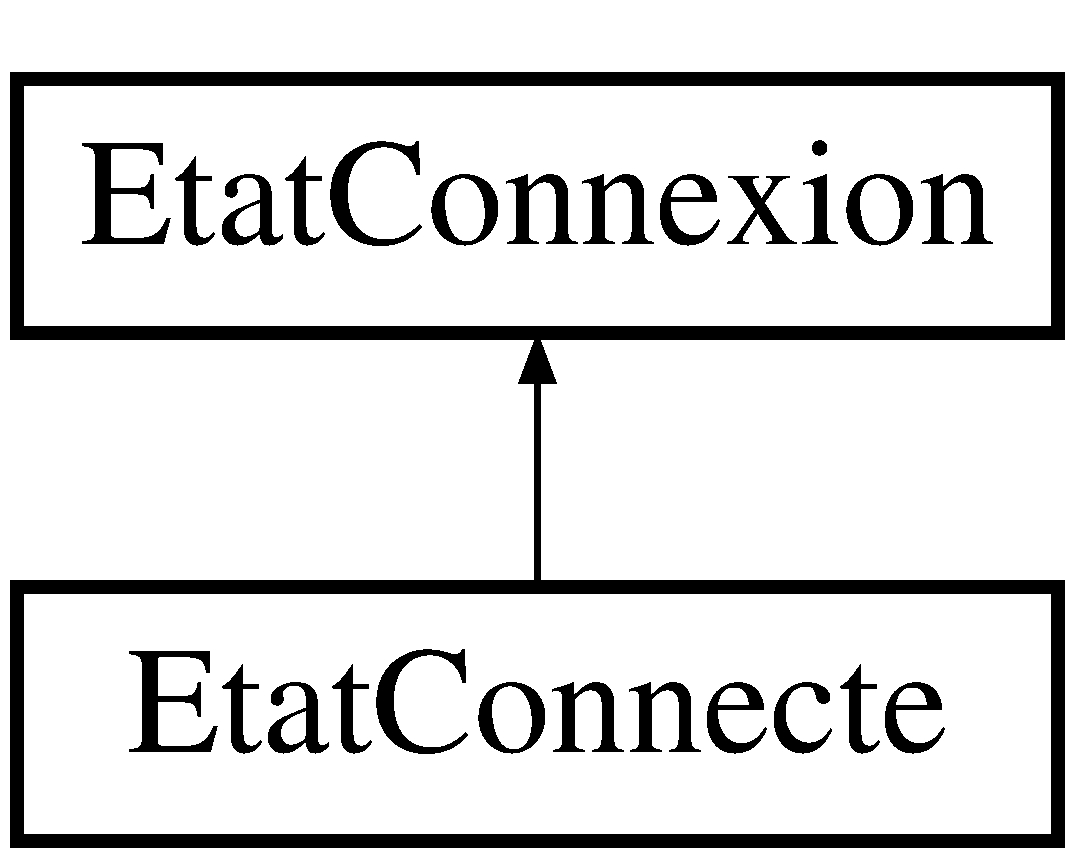
\includegraphics[height=2.000000cm]{class_etat_connecte}
\end{center}
\end{figure}
\subsection*{Fonctions membres publiques}
\begin{DoxyCompactItemize}
\item 
\hyperlink{class_etat_connecte_ab6bab0d2f0717b3803f75efe27e1915a}{Etat\-Connecte} (bool b)
\begin{DoxyCompactList}\small\item\em Constructeur de la classe \hyperlink{class_etat_connecte}{Etat\-Connecte}. \end{DoxyCompactList}\item 
virtual \hyperlink{class_etat_connecte_acc23dcca21e5e3f3d1af41a6ae615e8b}{$\sim$\-Etat\-Connecte} ()
\end{DoxyCompactItemize}
\subsection*{Membres hérités additionnels}


\subsection{Description détaillée}
Cette classe gère les utilisateurs connectés. 

Elle hérite de la classe \hyperlink{class_etat_connexion}{Etat\-Connexion} 

\subsection{Documentation des constructeurs et destructeur}
\hypertarget{class_etat_connecte_ab6bab0d2f0717b3803f75efe27e1915a}{\index{Etat\-Connecte@{Etat\-Connecte}!Etat\-Connecte@{Etat\-Connecte}}
\index{Etat\-Connecte@{Etat\-Connecte}!EtatConnecte@{Etat\-Connecte}}
\subsubsection[{Etat\-Connecte}]{\setlength{\rightskip}{0pt plus 5cm}Etat\-Connecte\-::\-Etat\-Connecte (
\begin{DoxyParamCaption}
\item[{bool}]{b}
\end{DoxyParamCaption}
)\hspace{0.3cm}{\ttfamily [inline]}}}\label{class_etat_connecte_ab6bab0d2f0717b3803f75efe27e1915a}


Constructeur de la classe \hyperlink{class_etat_connecte}{Etat\-Connecte}. 


\begin{DoxyParams}{Paramètres}
{\em b} & -\/ Nouvel état de connexion \\
\hline
\end{DoxyParams}
\hypertarget{class_etat_connecte_acc23dcca21e5e3f3d1af41a6ae615e8b}{\index{Etat\-Connecte@{Etat\-Connecte}!$\sim$\-Etat\-Connecte@{$\sim$\-Etat\-Connecte}}
\index{$\sim$\-Etat\-Connecte@{$\sim$\-Etat\-Connecte}!EtatConnecte@{Etat\-Connecte}}
\subsubsection[{$\sim$\-Etat\-Connecte}]{\setlength{\rightskip}{0pt plus 5cm}virtual Etat\-Connecte\-::$\sim$\-Etat\-Connecte (
\begin{DoxyParamCaption}
{}
\end{DoxyParamCaption}
)\hspace{0.3cm}{\ttfamily [inline]}, {\ttfamily [virtual]}}}\label{class_etat_connecte_acc23dcca21e5e3f3d1af41a6ae615e8b}


La documentation de cette classe a été générée à partir du fichier suivant \-:\begin{DoxyCompactItemize}
\item 
/home/magalie/\-Bureau/\-S5/\-C\-P\-O\-O\-A/\-Projet/\-E-\/\-Marche-\//iterations/iteration3/\-E\-Marche/bdd/\hyperlink{_etat_connecte_8h}{Etat\-Connecte.\-h}\end{DoxyCompactItemize}

\section{Etat\-Connexion Class Reference}
\label{class_etat_connexion}\index{Etat\-Connexion@{Etat\-Connexion}}
Inheritance diagram for Etat\-Connexion\-:\begin{figure}[H]
\begin{center}
\leavevmode
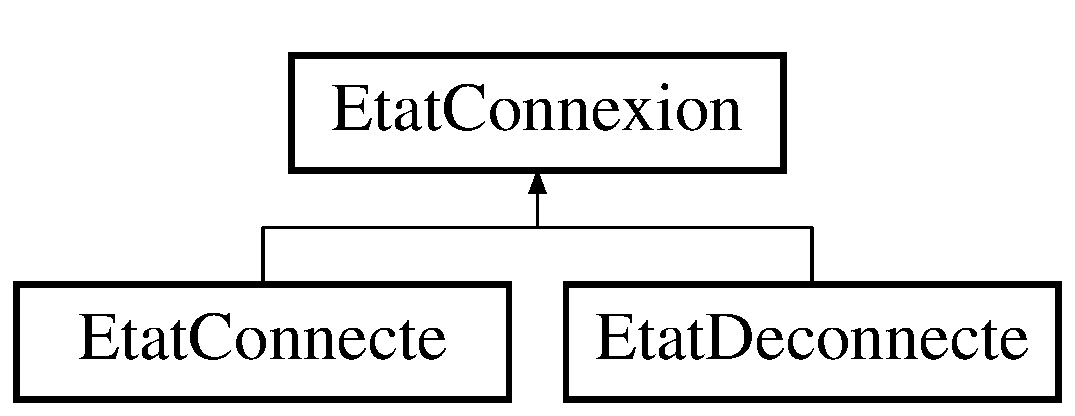
\includegraphics[height=2.000000cm]{class_etat_connexion}
\end{center}
\end{figure}
\subsection*{Public Member Functions}
\begin{DoxyCompactItemize}
\item 
{\bfseries Etat\-Connexion} (bool b)\label{class_etat_connexion_ab2f7cac2d3fb8ca6b89a6e9ae65262b5}

\item 
bool {\bfseries connexion\-En\-Cours} ()\label{class_etat_connexion_acbb22c19f9b8fb864cd783c51f725c6e}

\end{DoxyCompactItemize}


The documentation for this class was generated from the following files\-:\begin{DoxyCompactItemize}
\item 
Etat\-Connexion.\-h\item 
Etat\-Connexion.\-cpp\end{DoxyCompactItemize}

\hypertarget{class_etat_deconnecte}{\section{Référence de la classe Etat\-Deconnecte}
\label{class_etat_deconnecte}\index{Etat\-Deconnecte@{Etat\-Deconnecte}}
}


Cette classe gère les utilisateurs déconnectés.  




{\ttfamily \#include $<$Etat\-Deconnecte.\-h$>$}

Graphe d'héritage de Etat\-Deconnecte\-:\begin{figure}[H]
\begin{center}
\leavevmode
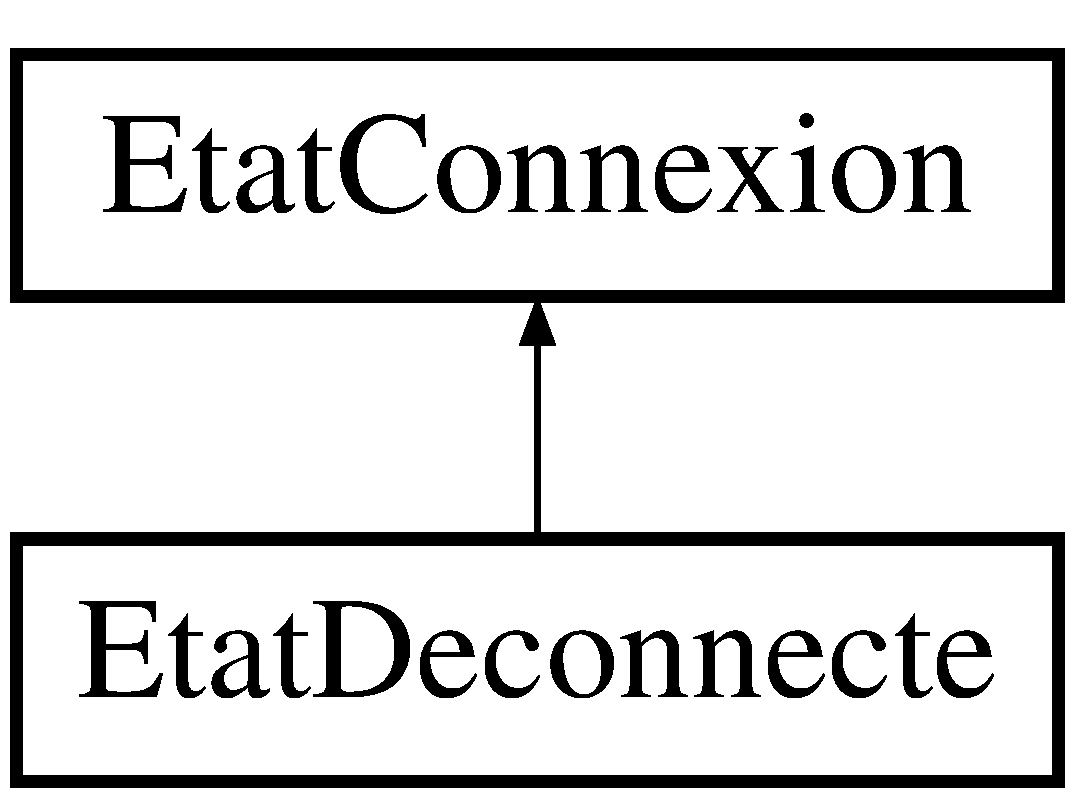
\includegraphics[height=2.000000cm]{class_etat_deconnecte}
\end{center}
\end{figure}
\subsection*{Fonctions membres publiques}
\begin{DoxyCompactItemize}
\item 
\hyperlink{class_etat_deconnecte_add0d9bf610ab5ca451880beacd6f0490}{Etat\-Deconnecte} (bool b)
\begin{DoxyCompactList}\small\item\em Constructeur de la classe \hyperlink{class_etat_deconnecte}{Etat\-Deconnecte}. \end{DoxyCompactList}\item 
virtual \hyperlink{class_etat_deconnecte_ad281d0077116df015bc1149557042d95}{$\sim$\-Etat\-Deconnecte} ()
\end{DoxyCompactItemize}
\subsection*{Membres hérités additionnels}


\subsection{Description détaillée}
Cette classe gère les utilisateurs déconnectés. 

Elle hérite de la classe \hyperlink{class_etat_connexion}{Etat\-Connexion} 

\subsection{Documentation des constructeurs et destructeur}
\hypertarget{class_etat_deconnecte_add0d9bf610ab5ca451880beacd6f0490}{\index{Etat\-Deconnecte@{Etat\-Deconnecte}!Etat\-Deconnecte@{Etat\-Deconnecte}}
\index{Etat\-Deconnecte@{Etat\-Deconnecte}!EtatDeconnecte@{Etat\-Deconnecte}}
\subsubsection[{Etat\-Deconnecte}]{\setlength{\rightskip}{0pt plus 5cm}Etat\-Deconnecte\-::\-Etat\-Deconnecte (
\begin{DoxyParamCaption}
\item[{bool}]{b}
\end{DoxyParamCaption}
)\hspace{0.3cm}{\ttfamily [inline]}}}\label{class_etat_deconnecte_add0d9bf610ab5ca451880beacd6f0490}


Constructeur de la classe \hyperlink{class_etat_deconnecte}{Etat\-Deconnecte}. 


\begin{DoxyParams}{Paramètres}
{\em b} & -\/ Nouvel état de connexion \\
\hline
\end{DoxyParams}
\hypertarget{class_etat_deconnecte_ad281d0077116df015bc1149557042d95}{\index{Etat\-Deconnecte@{Etat\-Deconnecte}!$\sim$\-Etat\-Deconnecte@{$\sim$\-Etat\-Deconnecte}}
\index{$\sim$\-Etat\-Deconnecte@{$\sim$\-Etat\-Deconnecte}!EtatDeconnecte@{Etat\-Deconnecte}}
\subsubsection[{$\sim$\-Etat\-Deconnecte}]{\setlength{\rightskip}{0pt plus 5cm}virtual Etat\-Deconnecte\-::$\sim$\-Etat\-Deconnecte (
\begin{DoxyParamCaption}
{}
\end{DoxyParamCaption}
)\hspace{0.3cm}{\ttfamily [inline]}, {\ttfamily [virtual]}}}\label{class_etat_deconnecte_ad281d0077116df015bc1149557042d95}


La documentation de cette classe a été générée à partir du fichier suivant \-:\begin{DoxyCompactItemize}
\item 
/home/magalie/\-Bureau/\-S5/\-C\-P\-O\-O\-A/\-Projet/\-E-\/\-Marche-\//iterations/iteration2/\-E\-Marche/bdd/\hyperlink{_etat_deconnecte_8h}{Etat\-Deconnecte.\-h}\end{DoxyCompactItemize}

\hypertarget{class_etat_vente}{\section{Référence de la classe Etat\-Vente}
\label{class_etat_vente}\index{Etat\-Vente@{Etat\-Vente}}
}


Cette classe gère l'état d'une vente (enchère ou normale)  




{\ttfamily \#include $<$Etat\-Vente.\-h$>$}

Graphe d'héritage de Etat\-Vente\-:\begin{figure}[H]
\begin{center}
\leavevmode
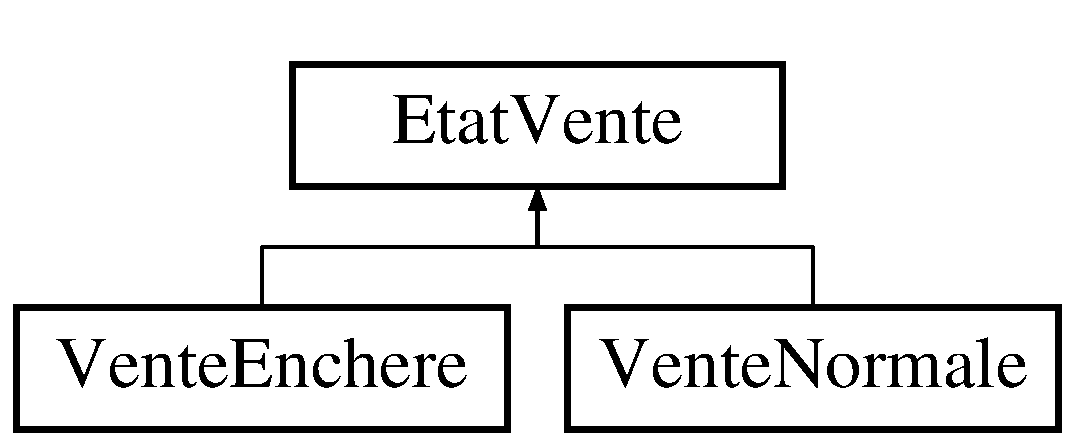
\includegraphics[height=2.000000cm]{class_etat_vente}
\end{center}
\end{figure}
\subsection*{Fonctions membres publiques}
\begin{DoxyCompactItemize}
\item 
\hyperlink{class_etat_vente_a6b2788e1edd74d8051623e966c5400a1}{Etat\-Vente} (bool b)
\begin{DoxyCompactList}\small\item\em Constructeur de la classe \hyperlink{class_etat_vente}{Etat\-Vente}. \end{DoxyCompactList}\item 
virtual \hyperlink{class_etat_vente_aace2ed3063f41ff36bddc3c09c024424}{$\sim$\-Etat\-Vente} ()
\item 
bool \hyperlink{class_etat_vente_acecfe3b215062d9a835831989e420ccd}{type\-Vente} ()
\begin{DoxyCompactList}\small\item\em Cette fonction indique la type de la vente. Si elle retourne true, c'est une vente aux enchères, sinon c'est une vente normale. \end{DoxyCompactList}\item 
virtual float \hyperlink{class_etat_vente_a0e797a253bbfe990d22f3d2827c8a318}{get\-Prix\-Actuel} ()
\begin{DoxyCompactList}\small\item\em Cette fonction virtuelle retourne le prix actuel de la vente. \end{DoxyCompactList}\item 
virtual std\-::string \hyperlink{class_etat_vente_ab466d257671a59ec97ae393c80226b7a}{get\-Date\-Limite} ()
\begin{DoxyCompactList}\small\item\em Cette fonction virtuelle retourne la date limite de l'enchère. \end{DoxyCompactList}\item 
virtual void \hyperlink{class_etat_vente_a8436bb978172c8e136fa349706baef0d}{set\-Prix\-Actuel} (float prix)
\begin{DoxyCompactList}\small\item\em Cette fonction virtuelle fixe le prix actuel. \end{DoxyCompactList}\item 
virtual void \hyperlink{class_etat_vente_a8efa95982f7252801512df1ea16faeeb}{set\-Date\-Limite} (struct tm date)
\begin{DoxyCompactList}\small\item\em Cette fonction virtuelle fixe la date limite. \end{DoxyCompactList}\end{DoxyCompactItemize}
\subsection*{Attributs protégés}
\begin{DoxyCompactItemize}
\item 
bool \hyperlink{class_etat_vente_a6fac909bb6c53a68450ff1f1e287e298}{type\-De\-Vente}
\begin{DoxyCompactList}\small\item\em Booléen qui distingue une vente normale d'une vente aux enchères. \end{DoxyCompactList}\item 
float \hyperlink{class_etat_vente_a69258e9f4890fc1fe84e5afdba35bc0f}{prix\-Actuel}
\begin{DoxyCompactList}\small\item\em Prix actuel. \end{DoxyCompactList}\item 
struct tm \hyperlink{class_etat_vente_a02900fecb3074f37d5a6d0948975de03}{date\-Limite}
\begin{DoxyCompactList}\small\item\em Date limite avant la fin de l'enchère. \end{DoxyCompactList}\end{DoxyCompactItemize}


\subsection{Description détaillée}
Cette classe gère l'état d'une vente (enchère ou normale) 

\subsection{Documentation des constructeurs et destructeur}
\hypertarget{class_etat_vente_a6b2788e1edd74d8051623e966c5400a1}{\index{Etat\-Vente@{Etat\-Vente}!Etat\-Vente@{Etat\-Vente}}
\index{Etat\-Vente@{Etat\-Vente}!EtatVente@{Etat\-Vente}}
\subsubsection[{Etat\-Vente}]{\setlength{\rightskip}{0pt plus 5cm}Etat\-Vente\-::\-Etat\-Vente (
\begin{DoxyParamCaption}
\item[{bool}]{b}
\end{DoxyParamCaption}
)}}\label{class_etat_vente_a6b2788e1edd74d8051623e966c5400a1}


Constructeur de la classe \hyperlink{class_etat_vente}{Etat\-Vente}. 


\begin{DoxyParams}{Paramètres}
{\em b} & -\/ Booléen qui donne le type de la vente \\
\hline
\end{DoxyParams}
\hypertarget{class_etat_vente_aace2ed3063f41ff36bddc3c09c024424}{\index{Etat\-Vente@{Etat\-Vente}!$\sim$\-Etat\-Vente@{$\sim$\-Etat\-Vente}}
\index{$\sim$\-Etat\-Vente@{$\sim$\-Etat\-Vente}!EtatVente@{Etat\-Vente}}
\subsubsection[{$\sim$\-Etat\-Vente}]{\setlength{\rightskip}{0pt plus 5cm}virtual Etat\-Vente\-::$\sim$\-Etat\-Vente (
\begin{DoxyParamCaption}
{}
\end{DoxyParamCaption}
)\hspace{0.3cm}{\ttfamily [inline]}, {\ttfamily [virtual]}}}\label{class_etat_vente_aace2ed3063f41ff36bddc3c09c024424}


\subsection{Documentation des fonctions membres}
\hypertarget{class_etat_vente_ab466d257671a59ec97ae393c80226b7a}{\index{Etat\-Vente@{Etat\-Vente}!get\-Date\-Limite@{get\-Date\-Limite}}
\index{get\-Date\-Limite@{get\-Date\-Limite}!EtatVente@{Etat\-Vente}}
\subsubsection[{get\-Date\-Limite}]{\setlength{\rightskip}{0pt plus 5cm}std\-::string Etat\-Vente\-::get\-Date\-Limite (
\begin{DoxyParamCaption}
{}
\end{DoxyParamCaption}
)\hspace{0.3cm}{\ttfamily [virtual]}}}\label{class_etat_vente_ab466d257671a59ec97ae393c80226b7a}


Cette fonction virtuelle retourne la date limite de l'enchère. 

\begin{DoxyReturn}{Renvoie}
Un string contenant la date limite de l'enchère 
\end{DoxyReturn}


Réimplémentée dans \hyperlink{class_vente_enchere_a2ab7fb32692d9cb1d250b81f0f87dd88}{Vente\-Enchere}.

\hypertarget{class_etat_vente_a0e797a253bbfe990d22f3d2827c8a318}{\index{Etat\-Vente@{Etat\-Vente}!get\-Prix\-Actuel@{get\-Prix\-Actuel}}
\index{get\-Prix\-Actuel@{get\-Prix\-Actuel}!EtatVente@{Etat\-Vente}}
\subsubsection[{get\-Prix\-Actuel}]{\setlength{\rightskip}{0pt plus 5cm}float Etat\-Vente\-::get\-Prix\-Actuel (
\begin{DoxyParamCaption}
{}
\end{DoxyParamCaption}
)\hspace{0.3cm}{\ttfamily [virtual]}}}\label{class_etat_vente_a0e797a253bbfe990d22f3d2827c8a318}


Cette fonction virtuelle retourne le prix actuel de la vente. 

\begin{DoxyReturn}{Renvoie}
Un float représentant le prix actuel 
\end{DoxyReturn}


Réimplémentée dans \hyperlink{class_vente_enchere_a53455121f689127d4daf6123af1668f3}{Vente\-Enchere}.

\hypertarget{class_etat_vente_a8efa95982f7252801512df1ea16faeeb}{\index{Etat\-Vente@{Etat\-Vente}!set\-Date\-Limite@{set\-Date\-Limite}}
\index{set\-Date\-Limite@{set\-Date\-Limite}!EtatVente@{Etat\-Vente}}
\subsubsection[{set\-Date\-Limite}]{\setlength{\rightskip}{0pt plus 5cm}void Etat\-Vente\-::set\-Date\-Limite (
\begin{DoxyParamCaption}
\item[{struct tm}]{date}
\end{DoxyParamCaption}
)\hspace{0.3cm}{\ttfamily [virtual]}}}\label{class_etat_vente_a8efa95982f7252801512df1ea16faeeb}


Cette fonction virtuelle fixe la date limite. 


\begin{DoxyParams}{Paramètres}
{\em date} & -\/ Nouvelle date \\
\hline
\end{DoxyParams}


Réimplémentée dans \hyperlink{class_vente_enchere_a034150f779a519dfc4973a3fcfd0d23e}{Vente\-Enchere}.

\hypertarget{class_etat_vente_a8436bb978172c8e136fa349706baef0d}{\index{Etat\-Vente@{Etat\-Vente}!set\-Prix\-Actuel@{set\-Prix\-Actuel}}
\index{set\-Prix\-Actuel@{set\-Prix\-Actuel}!EtatVente@{Etat\-Vente}}
\subsubsection[{set\-Prix\-Actuel}]{\setlength{\rightskip}{0pt plus 5cm}void Etat\-Vente\-::set\-Prix\-Actuel (
\begin{DoxyParamCaption}
\item[{float}]{prix}
\end{DoxyParamCaption}
)\hspace{0.3cm}{\ttfamily [virtual]}}}\label{class_etat_vente_a8436bb978172c8e136fa349706baef0d}


Cette fonction virtuelle fixe le prix actuel. 


\begin{DoxyParams}{Paramètres}
{\em prix} & -\/ Nouveau prix \\
\hline
\end{DoxyParams}


Réimplémentée dans \hyperlink{class_vente_enchere_abad32fe0ea40ea89e1aef1621dc673e6}{Vente\-Enchere}.

\hypertarget{class_etat_vente_acecfe3b215062d9a835831989e420ccd}{\index{Etat\-Vente@{Etat\-Vente}!type\-Vente@{type\-Vente}}
\index{type\-Vente@{type\-Vente}!EtatVente@{Etat\-Vente}}
\subsubsection[{type\-Vente}]{\setlength{\rightskip}{0pt plus 5cm}bool Etat\-Vente\-::type\-Vente (
\begin{DoxyParamCaption}
{}
\end{DoxyParamCaption}
)}}\label{class_etat_vente_acecfe3b215062d9a835831989e420ccd}


Cette fonction indique la type de la vente. Si elle retourne true, c'est une vente aux enchères, sinon c'est une vente normale. 

\begin{DoxyReturn}{Renvoie}
True si c'est une vente aux enchères, false sinon 
\end{DoxyReturn}


\subsection{Documentation des données membres}
\hypertarget{class_etat_vente_a02900fecb3074f37d5a6d0948975de03}{\index{Etat\-Vente@{Etat\-Vente}!date\-Limite@{date\-Limite}}
\index{date\-Limite@{date\-Limite}!EtatVente@{Etat\-Vente}}
\subsubsection[{date\-Limite}]{\setlength{\rightskip}{0pt plus 5cm}struct tm Etat\-Vente\-::date\-Limite\hspace{0.3cm}{\ttfamily [protected]}}}\label{class_etat_vente_a02900fecb3074f37d5a6d0948975de03}


Date limite avant la fin de l'enchère. 

\hypertarget{class_etat_vente_a69258e9f4890fc1fe84e5afdba35bc0f}{\index{Etat\-Vente@{Etat\-Vente}!prix\-Actuel@{prix\-Actuel}}
\index{prix\-Actuel@{prix\-Actuel}!EtatVente@{Etat\-Vente}}
\subsubsection[{prix\-Actuel}]{\setlength{\rightskip}{0pt plus 5cm}float Etat\-Vente\-::prix\-Actuel\hspace{0.3cm}{\ttfamily [protected]}}}\label{class_etat_vente_a69258e9f4890fc1fe84e5afdba35bc0f}


Prix actuel. 

\hypertarget{class_etat_vente_a6fac909bb6c53a68450ff1f1e287e298}{\index{Etat\-Vente@{Etat\-Vente}!type\-De\-Vente@{type\-De\-Vente}}
\index{type\-De\-Vente@{type\-De\-Vente}!EtatVente@{Etat\-Vente}}
\subsubsection[{type\-De\-Vente}]{\setlength{\rightskip}{0pt plus 5cm}bool Etat\-Vente\-::type\-De\-Vente\hspace{0.3cm}{\ttfamily [protected]}}}\label{class_etat_vente_a6fac909bb6c53a68450ff1f1e287e298}


Booléen qui distingue une vente normale d'une vente aux enchères. 



La documentation de cette classe a été générée à partir des fichiers suivants \-:\begin{DoxyCompactItemize}
\item 
/home/magalie/\-Bureau/\-S5/\-C\-P\-O\-O\-A/\-Projet/\-E-\/\-Marche-\//code/\-E\-Marche/bdd/\hyperlink{_etat_vente_8h}{Etat\-Vente.\-h}\item 
/home/magalie/\-Bureau/\-S5/\-C\-P\-O\-O\-A/\-Projet/\-E-\/\-Marche-\//code/\-E\-Marche/bdd/\hyperlink{_etat_vente_8cpp}{Etat\-Vente.\-cpp}\end{DoxyCompactItemize}

\hypertarget{class_gestion_bdd}{\section{Référence de la classe Gestion\-Bdd}
\label{class_gestion_bdd}\index{Gestion\-Bdd@{Gestion\-Bdd}}
}


The \hyperlink{class_gestion_bdd}{Gestion\-Bdd} class -\/ Gère le stockage des utilisateurs, des produits, et la mise à jour des vues.  




{\ttfamily \#include $<$Gestion\-Bdd.\-h$>$}

\subsection*{Fonctions membres publiques}
\begin{DoxyCompactItemize}
\item 
\hyperlink{class_gestion_bdd_aec9ad935a7fafff545f62c8c1452e8db}{Gestion\-Bdd} ()
\begin{DoxyCompactList}\small\item\em \hyperlink{class_gestion_bdd}{Gestion\-Bdd} -\/ constructeur. \end{DoxyCompactList}\item 
\hyperlink{class_gestion_bdd_a4398ba38755e93b303635ac5bd2713c6}{$\sim$\-Gestion\-Bdd} ()
\item 
void \hyperlink{class_gestion_bdd_acdaf971b3644b2aebbbb65a75b3e6c4c}{incrementer\-Ref} ()
\begin{DoxyCompactList}\small\item\em incrémente la référence pour l'attribuer à un produit et qu'elle soit unique (version 1) \end{DoxyCompactList}\item 
std\-::string \hyperlink{class_gestion_bdd_a6169a8867e04bcc950fe2e0fb2a5621d}{generate\-Reference} ()
\begin{DoxyCompactList}\small\item\em génère une référence unique (version 2) \end{DoxyCompactList}\item 
void \hyperlink{class_gestion_bdd_a029ffbc385ac5bbb665101308ae82ba0}{add\-Vue} (\hyperlink{class_vue}{Vue} $\ast$v)
\begin{DoxyCompactList}\small\item\em ajoute une vue au vector contenant les vues \end{DoxyCompactList}\item 
void \hyperlink{class_gestion_bdd_a518211afbda535f9bcbf718254c7a6aa}{update} ()
\begin{DoxyCompactList}\small\item\em provoque la fonction update dans toutes les vues \end{DoxyCompactList}\item 
void \hyperlink{class_gestion_bdd_ae1beeb1b627cbf2e6d0b044c9821d05a}{set\-Quantite} (int qte)
\begin{DoxyCompactList}\small\item\em Cette fonction fixe la quantité du produit que l'on veut acheter. \end{DoxyCompactList}\item 
int \hyperlink{class_gestion_bdd_ad0e14c4312471baad8d525ae9c3b0952}{get\-Quantite} ()
\begin{DoxyCompactList}\small\item\em Cette fonction retourne la quantité du produit que l'on veut acheter. \end{DoxyCompactList}\item 
\hyperlink{class_produit}{Produit} $\ast$ \hyperlink{class_gestion_bdd_a247c81f14899ebdc9666f62e9da73361}{get\-Produit\-Courant} ()
\begin{DoxyCompactList}\small\item\em Cette fonction retourne le produit courant. \end{DoxyCompactList}\item 
void \hyperlink{class_gestion_bdd_acdf8fc7e874b0c24408aaf1121aafda6}{set\-Produit\-Courant} (\hyperlink{class_produit}{Produit} $\ast$p)
\begin{DoxyCompactList}\small\item\em Cette fonction fixe le produit courant lorsque l'on consulte la fiche d'un produit. \end{DoxyCompactList}\item 
void \hyperlink{class_gestion_bdd_a936ae71d7145692ec01ccb0f282d3b59}{connecter\-Utilisateur} (std\-::string pseudo, std\-::string mdp)
\begin{DoxyCompactList}\small\item\em connecte l'utilisateur avec ce pseudo et ce mot de passe s'il existe \end{DoxyCompactList}\item 
void \hyperlink{class_gestion_bdd_a0e99ded45980647e925295e8cd828004}{deconnecter\-Utilisateur} ()
\begin{DoxyCompactList}\small\item\em déconnecte l'utilisateur \end{DoxyCompactList}\item 
bool \hyperlink{class_gestion_bdd_a86ee63900b31ef17bf487ebc1abe8634}{is\-Connecte} ()
\begin{DoxyCompactList}\small\item\em retourne true si un utilisateur est connecté, false sinon \end{DoxyCompactList}\item 
\hyperlink{class_utilisateur}{Utilisateur} $\ast$ \hyperlink{class_gestion_bdd_a2ca66731bc3b85a279d5b140e63ba838}{get\-Utilisateur\-Connecte} ()
\begin{DoxyCompactList}\small\item\em récupère un pointeur vers l'utilisateur actuellement connecté \end{DoxyCompactList}\item 
void \hyperlink{class_gestion_bdd_a02f362c2dd2ca487922e00988f71281b}{inscrire} (std\-::string mon\-Pseudo, std\-::string mon\-Mdp, std\-::string name, std\-::string firstname, int jour\-Naiss, int mois\-Naiss, int annee\-Naiss, std\-::string mail, std\-::string adr, int code\-Postal)
\begin{DoxyCompactList}\small\item\em inscrire un nouvel utilisateur et le stocker dans utilisateurs \end{DoxyCompactList}\item 
void \hyperlink{class_gestion_bdd_a966846d69aa1cf0ed82ef74127e10883}{modifier\-Profil} (std\-::string nom, std\-::string prenom, std\-::string mail, int code\-Postal, std\-::string ville, std\-::string adresse)
\begin{DoxyCompactList}\small\item\em modifie le profil avec ces informations \end{DoxyCompactList}\item 
void \hyperlink{class_gestion_bdd_a039afce368e1b90cbc26334cb8c7d065}{acheter\-Produit} (\hyperlink{class_produit}{Produit} $\ast$p, int \hyperlink{class_gestion_bdd_aea2dfb9c9690c8aef62feb9936426588}{quantite})
\begin{DoxyCompactList}\small\item\em acheter\-Produit -\/ Acheter un produit, avec suppression du produit si la quantité arrive à 0 \end{DoxyCompactList}\item 
\hyperlink{class_utilisateur}{Utilisateur} $\ast$ \hyperlink{class_gestion_bdd_a59989c7d58166c7e4a451b77e56bb852}{rechercher\-Utilisateur} (std\-::string pseudo)
\begin{DoxyCompactList}\small\item\em recherche l'utilisateur avec ce pseudo \end{DoxyCompactList}\item 
std\-::vector$<$ \hyperlink{class_utilisateur}{Utilisateur} $\ast$ $>$ \hyperlink{class_gestion_bdd_a96636fecdc9750ebd4236b3c58aed84f}{rechercher\-Utilisateurs} (std\-::string pseudo)
\begin{DoxyCompactList}\small\item\em recherche les utilisateurs contenant ce pseudo \end{DoxyCompactList}\item 
void \hyperlink{class_gestion_bdd_ac8c3809d6de97f0e81cd5045a4a72c7e}{ajouter\-Vente} (std\-::string n, std\-::string cat, float prix, unsigned int qte, bool etat)
\begin{DoxyCompactList}\small\item\em ajoute un produit en vente normale avec ces caractéristiques \end{DoxyCompactList}\item 
void \hyperlink{class_gestion_bdd_af4e95573213751d5487464ff3e24cc98}{ajouter\-Vente} (std\-::string n, std\-::string cat, float prix, unsigned int qte, bool etat, struct tm date)
\begin{DoxyCompactList}\small\item\em ajoute un produit en vente aux enchères avec ces caractéristiques \end{DoxyCompactList}\item 
std\-::vector$<$ \hyperlink{class_produit}{Produit} $\ast$ $>$ \hyperlink{class_gestion_bdd_aa52e1f2d076c4e3f65162e9f28ed20fa}{ventes\-En\-Cours} ()
\begin{DoxyCompactList}\small\item\em rtourne les ventes en cours \end{DoxyCompactList}\item 
\hyperlink{class_produit}{Produit} $\ast$ \hyperlink{class_gestion_bdd_abf0ffd54c39d6dfe431fc8d556eb5c8d}{rechercher\-Produit} (std\-::string \hyperlink{class_gestion_bdd_ae9e26a2043f3e10fb773107809bfc007}{ref})
\begin{DoxyCompactList}\small\item\em recherche le produit avec cette référence \end{DoxyCompactList}\item 
std\-::vector$<$ \hyperlink{class_produit}{Produit} $\ast$ $>$ \hyperlink{class_gestion_bdd_aadc12bc0c3aee41bc56918e44b5d1085}{rechercher\-Tags} (std\-::string t)
\begin{DoxyCompactList}\small\item\em recherche un produit par tags (c'est à dire nom, catégorie) \end{DoxyCompactList}\end{DoxyCompactItemize}
\subsection*{Attributs protégés}
\begin{DoxyCompactItemize}
\item 
\hyperlink{class_les_utilisateurs}{Les\-Utilisateurs} \hyperlink{class_gestion_bdd_a43b0bcad5d1eb6ff51c78ceb6cdd972c}{utilisateurs}
\item 
\hyperlink{class_les_produits}{Les\-Produits} \hyperlink{class_gestion_bdd_a3d8399948251d113edf841e5122c51b8}{produits}
\item 
std\-::vector$<$ \hyperlink{class_vue}{Vue} $\ast$ $>$ \hyperlink{class_gestion_bdd_a44ea1efd29c4996b1dcba0bf428051a7}{vues}
\item 
\hyperlink{class_utilisateur}{Utilisateur} $\ast$ \hyperlink{class_gestion_bdd_adb07bb1f3015855aef7bcfe0b278ebd7}{utilisateur\-Connecte}
\item 
std\-::string \hyperlink{class_gestion_bdd_ae9e26a2043f3e10fb773107809bfc007}{ref}
\item 
int \hyperlink{class_gestion_bdd_aea2dfb9c9690c8aef62feb9936426588}{quantite}
\item 
\hyperlink{class_produit}{Produit} $\ast$ \hyperlink{class_gestion_bdd_a892f50933d1226a389b561276bd0ca93}{produit\-Courant}
\end{DoxyCompactItemize}


\subsection{Description détaillée}
The \hyperlink{class_gestion_bdd}{Gestion\-Bdd} class -\/ Gère le stockage des utilisateurs, des produits, et la mise à jour des vues. 

\subsection{Documentation des constructeurs et destructeur}
\hypertarget{class_gestion_bdd_aec9ad935a7fafff545f62c8c1452e8db}{\index{Gestion\-Bdd@{Gestion\-Bdd}!Gestion\-Bdd@{Gestion\-Bdd}}
\index{Gestion\-Bdd@{Gestion\-Bdd}!GestionBdd@{Gestion\-Bdd}}
\subsubsection[{Gestion\-Bdd}]{\setlength{\rightskip}{0pt plus 5cm}Gestion\-Bdd\-::\-Gestion\-Bdd (
\begin{DoxyParamCaption}
{}
\end{DoxyParamCaption}
)}}\label{class_gestion_bdd_aec9ad935a7fafff545f62c8c1452e8db}


\hyperlink{class_gestion_bdd}{Gestion\-Bdd} -\/ constructeur. 

\hypertarget{class_gestion_bdd_a4398ba38755e93b303635ac5bd2713c6}{\index{Gestion\-Bdd@{Gestion\-Bdd}!$\sim$\-Gestion\-Bdd@{$\sim$\-Gestion\-Bdd}}
\index{$\sim$\-Gestion\-Bdd@{$\sim$\-Gestion\-Bdd}!GestionBdd@{Gestion\-Bdd}}
\subsubsection[{$\sim$\-Gestion\-Bdd}]{\setlength{\rightskip}{0pt plus 5cm}Gestion\-Bdd\-::$\sim$\-Gestion\-Bdd (
\begin{DoxyParamCaption}
{}
\end{DoxyParamCaption}
)\hspace{0.3cm}{\ttfamily [inline]}}}\label{class_gestion_bdd_a4398ba38755e93b303635ac5bd2713c6}


\subsection{Documentation des fonctions membres}
\hypertarget{class_gestion_bdd_a039afce368e1b90cbc26334cb8c7d065}{\index{Gestion\-Bdd@{Gestion\-Bdd}!acheter\-Produit@{acheter\-Produit}}
\index{acheter\-Produit@{acheter\-Produit}!GestionBdd@{Gestion\-Bdd}}
\subsubsection[{acheter\-Produit}]{\setlength{\rightskip}{0pt plus 5cm}void Gestion\-Bdd\-::acheter\-Produit (
\begin{DoxyParamCaption}
\item[{{\bf Produit} $\ast$}]{p, }
\item[{int}]{quantite}
\end{DoxyParamCaption}
)}}\label{class_gestion_bdd_a039afce368e1b90cbc26334cb8c7d065}


acheter\-Produit -\/ Acheter un produit, avec suppression du produit si la quantité arrive à 0 


\begin{DoxyParams}{Paramètres}
{\em p} & -\/ Pointeur vers le produit à acheter \\
\hline
{\em quantite} & -\/ Quantité de produit acheté \\
\hline
\end{DoxyParams}
\hypertarget{class_gestion_bdd_a029ffbc385ac5bbb665101308ae82ba0}{\index{Gestion\-Bdd@{Gestion\-Bdd}!add\-Vue@{add\-Vue}}
\index{add\-Vue@{add\-Vue}!GestionBdd@{Gestion\-Bdd}}
\subsubsection[{add\-Vue}]{\setlength{\rightskip}{0pt plus 5cm}void Gestion\-Bdd\-::add\-Vue (
\begin{DoxyParamCaption}
\item[{{\bf Vue} $\ast$}]{v}
\end{DoxyParamCaption}
)}}\label{class_gestion_bdd_a029ffbc385ac5bbb665101308ae82ba0}


ajoute une vue au vector contenant les vues 


\begin{DoxyParams}{Paramètres}
{\em v} & -\/ pointeur vers la vue à ajouter \\
\hline
\end{DoxyParams}
\hypertarget{class_gestion_bdd_ac8c3809d6de97f0e81cd5045a4a72c7e}{\index{Gestion\-Bdd@{Gestion\-Bdd}!ajouter\-Vente@{ajouter\-Vente}}
\index{ajouter\-Vente@{ajouter\-Vente}!GestionBdd@{Gestion\-Bdd}}
\subsubsection[{ajouter\-Vente}]{\setlength{\rightskip}{0pt plus 5cm}void Gestion\-Bdd\-::ajouter\-Vente (
\begin{DoxyParamCaption}
\item[{std\-::string}]{n, }
\item[{std\-::string}]{cat, }
\item[{float}]{prix, }
\item[{unsigned int}]{qte, }
\item[{bool}]{etat}
\end{DoxyParamCaption}
)}}\label{class_gestion_bdd_ac8c3809d6de97f0e81cd5045a4a72c7e}


ajoute un produit en vente normale avec ces caractéristiques 


\begin{DoxyParams}{Paramètres}
{\em n} & -\/ nom du produit \\
\hline
{\em cat} & -\/ catégorie du produit \\
\hline
{\em prix} & -\/ prix du produit \\
\hline
{\em qte} & -\/ quantité du produit \\
\hline
{\em etat} & -\/ état du produit (en enchère ou non) \\
\hline
\end{DoxyParams}
\hypertarget{class_gestion_bdd_af4e95573213751d5487464ff3e24cc98}{\index{Gestion\-Bdd@{Gestion\-Bdd}!ajouter\-Vente@{ajouter\-Vente}}
\index{ajouter\-Vente@{ajouter\-Vente}!GestionBdd@{Gestion\-Bdd}}
\subsubsection[{ajouter\-Vente}]{\setlength{\rightskip}{0pt plus 5cm}void Gestion\-Bdd\-::ajouter\-Vente (
\begin{DoxyParamCaption}
\item[{std\-::string}]{n, }
\item[{std\-::string}]{cat, }
\item[{float}]{prix, }
\item[{unsigned int}]{qte, }
\item[{bool}]{etat, }
\item[{struct tm}]{date}
\end{DoxyParamCaption}
)}}\label{class_gestion_bdd_af4e95573213751d5487464ff3e24cc98}


ajoute un produit en vente aux enchères avec ces caractéristiques 


\begin{DoxyParams}{Paramètres}
{\em n} & -\/ nom du produit \\
\hline
{\em cat} & -\/ catégorie du produit \\
\hline
{\em prix} & -\/ prix du produit \\
\hline
{\em qte} & -\/ quantité du produit \\
\hline
{\em etat} & -\/ état du produit (enchère ou non) \\
\hline
{\em date} & -\/ date limite de l'enchère du produit \\
\hline
\end{DoxyParams}
\hypertarget{class_gestion_bdd_a936ae71d7145692ec01ccb0f282d3b59}{\index{Gestion\-Bdd@{Gestion\-Bdd}!connecter\-Utilisateur@{connecter\-Utilisateur}}
\index{connecter\-Utilisateur@{connecter\-Utilisateur}!GestionBdd@{Gestion\-Bdd}}
\subsubsection[{connecter\-Utilisateur}]{\setlength{\rightskip}{0pt plus 5cm}void Gestion\-Bdd\-::connecter\-Utilisateur (
\begin{DoxyParamCaption}
\item[{std\-::string}]{pseudo, }
\item[{std\-::string}]{mdp}
\end{DoxyParamCaption}
)}}\label{class_gestion_bdd_a936ae71d7145692ec01ccb0f282d3b59}


connecte l'utilisateur avec ce pseudo et ce mot de passe s'il existe 


\begin{DoxyParams}{Paramètres}
{\em pseudo} & -\/ pseudo de l'utilisateur qui veut se connecter \\
\hline
{\em mdp} & -\/ mot de passe de l'utilisateur qui veut se connecter \\
\hline
\end{DoxyParams}
\hypertarget{class_gestion_bdd_a0e99ded45980647e925295e8cd828004}{\index{Gestion\-Bdd@{Gestion\-Bdd}!deconnecter\-Utilisateur@{deconnecter\-Utilisateur}}
\index{deconnecter\-Utilisateur@{deconnecter\-Utilisateur}!GestionBdd@{Gestion\-Bdd}}
\subsubsection[{deconnecter\-Utilisateur}]{\setlength{\rightskip}{0pt plus 5cm}void Gestion\-Bdd\-::deconnecter\-Utilisateur (
\begin{DoxyParamCaption}
{}
\end{DoxyParamCaption}
)}}\label{class_gestion_bdd_a0e99ded45980647e925295e8cd828004}


déconnecte l'utilisateur 

\hypertarget{class_gestion_bdd_a6169a8867e04bcc950fe2e0fb2a5621d}{\index{Gestion\-Bdd@{Gestion\-Bdd}!generate\-Reference@{generate\-Reference}}
\index{generate\-Reference@{generate\-Reference}!GestionBdd@{Gestion\-Bdd}}
\subsubsection[{generate\-Reference}]{\setlength{\rightskip}{0pt plus 5cm}std\-::string Gestion\-Bdd\-::generate\-Reference (
\begin{DoxyParamCaption}
{}
\end{DoxyParamCaption}
)}}\label{class_gestion_bdd_a6169a8867e04bcc950fe2e0fb2a5621d}


génère une référence unique (version 2) 

\begin{DoxyReturn}{Renvoie}
std\-::string -\/ référence 
\end{DoxyReturn}
\hypertarget{class_gestion_bdd_a247c81f14899ebdc9666f62e9da73361}{\index{Gestion\-Bdd@{Gestion\-Bdd}!get\-Produit\-Courant@{get\-Produit\-Courant}}
\index{get\-Produit\-Courant@{get\-Produit\-Courant}!GestionBdd@{Gestion\-Bdd}}
\subsubsection[{get\-Produit\-Courant}]{\setlength{\rightskip}{0pt plus 5cm}{\bf Produit} $\ast$ Gestion\-Bdd\-::get\-Produit\-Courant (
\begin{DoxyParamCaption}
{}
\end{DoxyParamCaption}
)}}\label{class_gestion_bdd_a247c81f14899ebdc9666f62e9da73361}


Cette fonction retourne le produit courant. 

\begin{DoxyReturn}{Renvoie}
Le produit courant 
\end{DoxyReturn}
\hypertarget{class_gestion_bdd_ad0e14c4312471baad8d525ae9c3b0952}{\index{Gestion\-Bdd@{Gestion\-Bdd}!get\-Quantite@{get\-Quantite}}
\index{get\-Quantite@{get\-Quantite}!GestionBdd@{Gestion\-Bdd}}
\subsubsection[{get\-Quantite}]{\setlength{\rightskip}{0pt plus 5cm}int Gestion\-Bdd\-::get\-Quantite (
\begin{DoxyParamCaption}
{}
\end{DoxyParamCaption}
)}}\label{class_gestion_bdd_ad0e14c4312471baad8d525ae9c3b0952}


Cette fonction retourne la quantité du produit que l'on veut acheter. 

\begin{DoxyReturn}{Renvoie}
Un entier 
\end{DoxyReturn}
\hypertarget{class_gestion_bdd_a2ca66731bc3b85a279d5b140e63ba838}{\index{Gestion\-Bdd@{Gestion\-Bdd}!get\-Utilisateur\-Connecte@{get\-Utilisateur\-Connecte}}
\index{get\-Utilisateur\-Connecte@{get\-Utilisateur\-Connecte}!GestionBdd@{Gestion\-Bdd}}
\subsubsection[{get\-Utilisateur\-Connecte}]{\setlength{\rightskip}{0pt plus 5cm}{\bf Utilisateur} $\ast$ Gestion\-Bdd\-::get\-Utilisateur\-Connecte (
\begin{DoxyParamCaption}
{}
\end{DoxyParamCaption}
)}}\label{class_gestion_bdd_a2ca66731bc3b85a279d5b140e63ba838}


récupère un pointeur vers l'utilisateur actuellement connecté 

\begin{DoxyReturn}{Renvoie}
pointeur vers l'utilisateur connecté 
\end{DoxyReturn}
\hypertarget{class_gestion_bdd_acdaf971b3644b2aebbbb65a75b3e6c4c}{\index{Gestion\-Bdd@{Gestion\-Bdd}!incrementer\-Ref@{incrementer\-Ref}}
\index{incrementer\-Ref@{incrementer\-Ref}!GestionBdd@{Gestion\-Bdd}}
\subsubsection[{incrementer\-Ref}]{\setlength{\rightskip}{0pt plus 5cm}void Gestion\-Bdd\-::incrementer\-Ref (
\begin{DoxyParamCaption}
{}
\end{DoxyParamCaption}
)}}\label{class_gestion_bdd_acdaf971b3644b2aebbbb65a75b3e6c4c}


incrémente la référence pour l'attribuer à un produit et qu'elle soit unique (version 1) 

\hypertarget{class_gestion_bdd_a02f362c2dd2ca487922e00988f71281b}{\index{Gestion\-Bdd@{Gestion\-Bdd}!inscrire@{inscrire}}
\index{inscrire@{inscrire}!GestionBdd@{Gestion\-Bdd}}
\subsubsection[{inscrire}]{\setlength{\rightskip}{0pt plus 5cm}void Gestion\-Bdd\-::inscrire (
\begin{DoxyParamCaption}
\item[{std\-::string}]{mon\-Pseudo, }
\item[{std\-::string}]{mon\-Mdp, }
\item[{std\-::string}]{name, }
\item[{std\-::string}]{firstname, }
\item[{int}]{jour\-Naiss, }
\item[{int}]{mois\-Naiss, }
\item[{int}]{annee\-Naiss, }
\item[{std\-::string}]{mail, }
\item[{std\-::string}]{adr, }
\item[{int}]{code\-Postal}
\end{DoxyParamCaption}
)}}\label{class_gestion_bdd_a02f362c2dd2ca487922e00988f71281b}


inscrire un nouvel utilisateur et le stocker dans utilisateurs 


\begin{DoxyParams}{Paramètres}
{\em mon\-Pseudo} & -\/ pseudo de l'utilisateur à inscrire \\
\hline
{\em mon\-Mdp} & -\/ mot de passe de l'utilisateur à inscrire \\
\hline
{\em name} & -\/ nom de l'utilisateur à inscrire \\
\hline
{\em firstname} & -\/ prenom de l'utilisateur à inscrire \\
\hline
{\em jour\-Naiss} & -\/ jour de la date de naissance de l'utilisateur à inscrire \\
\hline
{\em mois\-Naiss} & -\/ mois de la date de naissance de l'utilisateur à inscrire \\
\hline
{\em annee\-Naiss} & -\/ année de la date de naissance de l'utilisateur à inscrire \\
\hline
{\em mail} & -\/ adresse mail de l'utilisateur à inscrire \\
\hline
{\em adr} & -\/ adresse de l'utilisateur à inscrire \\
\hline
{\em code\-Postal} & -\/ code postal de l'utilisateur à inscrire \\
\hline
\end{DoxyParams}
\hypertarget{class_gestion_bdd_a86ee63900b31ef17bf487ebc1abe8634}{\index{Gestion\-Bdd@{Gestion\-Bdd}!is\-Connecte@{is\-Connecte}}
\index{is\-Connecte@{is\-Connecte}!GestionBdd@{Gestion\-Bdd}}
\subsubsection[{is\-Connecte}]{\setlength{\rightskip}{0pt plus 5cm}bool Gestion\-Bdd\-::is\-Connecte (
\begin{DoxyParamCaption}
{}
\end{DoxyParamCaption}
)}}\label{class_gestion_bdd_a86ee63900b31ef17bf487ebc1abe8634}


retourne true si un utilisateur est connecté, false sinon 

\begin{DoxyReturn}{Renvoie}
true si un utilisateur est connecté, false sinon 
\end{DoxyReturn}
\hypertarget{class_gestion_bdd_a966846d69aa1cf0ed82ef74127e10883}{\index{Gestion\-Bdd@{Gestion\-Bdd}!modifier\-Profil@{modifier\-Profil}}
\index{modifier\-Profil@{modifier\-Profil}!GestionBdd@{Gestion\-Bdd}}
\subsubsection[{modifier\-Profil}]{\setlength{\rightskip}{0pt plus 5cm}void Gestion\-Bdd\-::modifier\-Profil (
\begin{DoxyParamCaption}
\item[{std\-::string}]{nom, }
\item[{std\-::string}]{prenom, }
\item[{std\-::string}]{mail, }
\item[{int}]{code\-Postal, }
\item[{std\-::string}]{ville, }
\item[{std\-::string}]{adresse}
\end{DoxyParamCaption}
)}}\label{class_gestion_bdd_a966846d69aa1cf0ed82ef74127e10883}


modifie le profil avec ces informations 


\begin{DoxyParams}{Paramètres}
{\em nom} & -\/ nouveau nom \\
\hline
{\em prenom} & -\/ nouveau prénom \\
\hline
{\em mail} & -\/ nouvelle adresse mail \\
\hline
{\em code\-Postal} & -\/ nouveau code postal \\
\hline
{\em ville} & -\/ nouvelle ville \\
\hline
{\em adresse} & -\/ nouvelle adresse \\
\hline
\end{DoxyParams}
\hypertarget{class_gestion_bdd_abf0ffd54c39d6dfe431fc8d556eb5c8d}{\index{Gestion\-Bdd@{Gestion\-Bdd}!rechercher\-Produit@{rechercher\-Produit}}
\index{rechercher\-Produit@{rechercher\-Produit}!GestionBdd@{Gestion\-Bdd}}
\subsubsection[{rechercher\-Produit}]{\setlength{\rightskip}{0pt plus 5cm}{\bf Produit} $\ast$ Gestion\-Bdd\-::rechercher\-Produit (
\begin{DoxyParamCaption}
\item[{std\-::string}]{ref}
\end{DoxyParamCaption}
)}}\label{class_gestion_bdd_abf0ffd54c39d6dfe431fc8d556eb5c8d}


recherche le produit avec cette référence 


\begin{DoxyParams}{Paramètres}
{\em ref} & -\/ référence du produit recherché \\
\hline
\end{DoxyParams}
\begin{DoxyReturn}{Renvoie}
le produit recherché 
\end{DoxyReturn}
\hypertarget{class_gestion_bdd_aadc12bc0c3aee41bc56918e44b5d1085}{\index{Gestion\-Bdd@{Gestion\-Bdd}!rechercher\-Tags@{rechercher\-Tags}}
\index{rechercher\-Tags@{rechercher\-Tags}!GestionBdd@{Gestion\-Bdd}}
\subsubsection[{rechercher\-Tags}]{\setlength{\rightskip}{0pt plus 5cm}std\-::vector$<$ {\bf Produit} $\ast$ $>$ Gestion\-Bdd\-::rechercher\-Tags (
\begin{DoxyParamCaption}
\item[{std\-::string}]{t}
\end{DoxyParamCaption}
)}}\label{class_gestion_bdd_aadc12bc0c3aee41bc56918e44b5d1085}


recherche un produit par tags (c'est à dire nom, catégorie) 


\begin{DoxyParams}{Paramètres}
{\em t} & -\/ tags recherchés \\
\hline
\end{DoxyParams}
\begin{DoxyReturn}{Renvoie}
un vector contenant des pointeurs sur les produits trouvés 
\end{DoxyReturn}
\hypertarget{class_gestion_bdd_a59989c7d58166c7e4a451b77e56bb852}{\index{Gestion\-Bdd@{Gestion\-Bdd}!rechercher\-Utilisateur@{rechercher\-Utilisateur}}
\index{rechercher\-Utilisateur@{rechercher\-Utilisateur}!GestionBdd@{Gestion\-Bdd}}
\subsubsection[{rechercher\-Utilisateur}]{\setlength{\rightskip}{0pt plus 5cm}{\bf Utilisateur} $\ast$ Gestion\-Bdd\-::rechercher\-Utilisateur (
\begin{DoxyParamCaption}
\item[{std\-::string}]{pseudo}
\end{DoxyParamCaption}
)}}\label{class_gestion_bdd_a59989c7d58166c7e4a451b77e56bb852}


recherche l'utilisateur avec ce pseudo 


\begin{DoxyParams}{Paramètres}
{\em pseudo} & -\/ pseudo recherché \\
\hline
\end{DoxyParams}
\begin{DoxyReturn}{Renvoie}
un pointeur vers l'utilisateur recherché 
\end{DoxyReturn}
\hypertarget{class_gestion_bdd_a96636fecdc9750ebd4236b3c58aed84f}{\index{Gestion\-Bdd@{Gestion\-Bdd}!rechercher\-Utilisateurs@{rechercher\-Utilisateurs}}
\index{rechercher\-Utilisateurs@{rechercher\-Utilisateurs}!GestionBdd@{Gestion\-Bdd}}
\subsubsection[{rechercher\-Utilisateurs}]{\setlength{\rightskip}{0pt plus 5cm}std\-::vector$<$ {\bf Utilisateur} $\ast$ $>$ Gestion\-Bdd\-::rechercher\-Utilisateurs (
\begin{DoxyParamCaption}
\item[{std\-::string}]{pseudo}
\end{DoxyParamCaption}
)}}\label{class_gestion_bdd_a96636fecdc9750ebd4236b3c58aed84f}


recherche les utilisateurs contenant ce pseudo 


\begin{DoxyParams}{Paramètres}
{\em pseudo} & -\/ pseudo recherché \\
\hline
\end{DoxyParams}
\begin{DoxyReturn}{Renvoie}
vector de pointeurs vers les utilisateurs trouvés 
\end{DoxyReturn}
\hypertarget{class_gestion_bdd_acdf8fc7e874b0c24408aaf1121aafda6}{\index{Gestion\-Bdd@{Gestion\-Bdd}!set\-Produit\-Courant@{set\-Produit\-Courant}}
\index{set\-Produit\-Courant@{set\-Produit\-Courant}!GestionBdd@{Gestion\-Bdd}}
\subsubsection[{set\-Produit\-Courant}]{\setlength{\rightskip}{0pt plus 5cm}void Gestion\-Bdd\-::set\-Produit\-Courant (
\begin{DoxyParamCaption}
\item[{{\bf Produit} $\ast$}]{p}
\end{DoxyParamCaption}
)}}\label{class_gestion_bdd_acdf8fc7e874b0c24408aaf1121aafda6}


Cette fonction fixe le produit courant lorsque l'on consulte la fiche d'un produit. 


\begin{DoxyParams}{Paramètres}
{\em p} & -\/ \hyperlink{class_produit}{Produit} consulté \\
\hline
\end{DoxyParams}
\hypertarget{class_gestion_bdd_ae1beeb1b627cbf2e6d0b044c9821d05a}{\index{Gestion\-Bdd@{Gestion\-Bdd}!set\-Quantite@{set\-Quantite}}
\index{set\-Quantite@{set\-Quantite}!GestionBdd@{Gestion\-Bdd}}
\subsubsection[{set\-Quantite}]{\setlength{\rightskip}{0pt plus 5cm}void Gestion\-Bdd\-::set\-Quantite (
\begin{DoxyParamCaption}
\item[{int}]{qte}
\end{DoxyParamCaption}
)}}\label{class_gestion_bdd_ae1beeb1b627cbf2e6d0b044c9821d05a}


Cette fonction fixe la quantité du produit que l'on veut acheter. 


\begin{DoxyParams}{Paramètres}
{\em qte} & \\
\hline
\end{DoxyParams}
\hypertarget{class_gestion_bdd_a518211afbda535f9bcbf718254c7a6aa}{\index{Gestion\-Bdd@{Gestion\-Bdd}!update@{update}}
\index{update@{update}!GestionBdd@{Gestion\-Bdd}}
\subsubsection[{update}]{\setlength{\rightskip}{0pt plus 5cm}void Gestion\-Bdd\-::update (
\begin{DoxyParamCaption}
{}
\end{DoxyParamCaption}
)}}\label{class_gestion_bdd_a518211afbda535f9bcbf718254c7a6aa}


provoque la fonction update dans toutes les vues 

\hypertarget{class_gestion_bdd_aa52e1f2d076c4e3f65162e9f28ed20fa}{\index{Gestion\-Bdd@{Gestion\-Bdd}!ventes\-En\-Cours@{ventes\-En\-Cours}}
\index{ventes\-En\-Cours@{ventes\-En\-Cours}!GestionBdd@{Gestion\-Bdd}}
\subsubsection[{ventes\-En\-Cours}]{\setlength{\rightskip}{0pt plus 5cm}std\-::vector$<$ {\bf Produit} $\ast$ $>$ Gestion\-Bdd\-::ventes\-En\-Cours (
\begin{DoxyParamCaption}
{}
\end{DoxyParamCaption}
)}}\label{class_gestion_bdd_aa52e1f2d076c4e3f65162e9f28ed20fa}


rtourne les ventes en cours 

\begin{DoxyReturn}{Renvoie}
un vector contenant des pointeurs vers les produits en vente 
\end{DoxyReturn}


\subsection{Documentation des données membres}
\hypertarget{class_gestion_bdd_a892f50933d1226a389b561276bd0ca93}{\index{Gestion\-Bdd@{Gestion\-Bdd}!produit\-Courant@{produit\-Courant}}
\index{produit\-Courant@{produit\-Courant}!GestionBdd@{Gestion\-Bdd}}
\subsubsection[{produit\-Courant}]{\setlength{\rightskip}{0pt plus 5cm}{\bf Produit}$\ast$ Gestion\-Bdd\-::produit\-Courant\hspace{0.3cm}{\ttfamily [protected]}}}\label{class_gestion_bdd_a892f50933d1226a389b561276bd0ca93}
\hypertarget{class_gestion_bdd_a3d8399948251d113edf841e5122c51b8}{\index{Gestion\-Bdd@{Gestion\-Bdd}!produits@{produits}}
\index{produits@{produits}!GestionBdd@{Gestion\-Bdd}}
\subsubsection[{produits}]{\setlength{\rightskip}{0pt plus 5cm}{\bf Les\-Produits} Gestion\-Bdd\-::produits\hspace{0.3cm}{\ttfamily [protected]}}}\label{class_gestion_bdd_a3d8399948251d113edf841e5122c51b8}
\hypertarget{class_gestion_bdd_aea2dfb9c9690c8aef62feb9936426588}{\index{Gestion\-Bdd@{Gestion\-Bdd}!quantite@{quantite}}
\index{quantite@{quantite}!GestionBdd@{Gestion\-Bdd}}
\subsubsection[{quantite}]{\setlength{\rightskip}{0pt plus 5cm}int Gestion\-Bdd\-::quantite\hspace{0.3cm}{\ttfamily [protected]}}}\label{class_gestion_bdd_aea2dfb9c9690c8aef62feb9936426588}
\hypertarget{class_gestion_bdd_ae9e26a2043f3e10fb773107809bfc007}{\index{Gestion\-Bdd@{Gestion\-Bdd}!ref@{ref}}
\index{ref@{ref}!GestionBdd@{Gestion\-Bdd}}
\subsubsection[{ref}]{\setlength{\rightskip}{0pt plus 5cm}std\-::string Gestion\-Bdd\-::ref\hspace{0.3cm}{\ttfamily [protected]}}}\label{class_gestion_bdd_ae9e26a2043f3e10fb773107809bfc007}
\hypertarget{class_gestion_bdd_adb07bb1f3015855aef7bcfe0b278ebd7}{\index{Gestion\-Bdd@{Gestion\-Bdd}!utilisateur\-Connecte@{utilisateur\-Connecte}}
\index{utilisateur\-Connecte@{utilisateur\-Connecte}!GestionBdd@{Gestion\-Bdd}}
\subsubsection[{utilisateur\-Connecte}]{\setlength{\rightskip}{0pt plus 5cm}{\bf Utilisateur}$\ast$ Gestion\-Bdd\-::utilisateur\-Connecte\hspace{0.3cm}{\ttfamily [protected]}}}\label{class_gestion_bdd_adb07bb1f3015855aef7bcfe0b278ebd7}
\hypertarget{class_gestion_bdd_a43b0bcad5d1eb6ff51c78ceb6cdd972c}{\index{Gestion\-Bdd@{Gestion\-Bdd}!utilisateurs@{utilisateurs}}
\index{utilisateurs@{utilisateurs}!GestionBdd@{Gestion\-Bdd}}
\subsubsection[{utilisateurs}]{\setlength{\rightskip}{0pt plus 5cm}{\bf Les\-Utilisateurs} Gestion\-Bdd\-::utilisateurs\hspace{0.3cm}{\ttfamily [protected]}}}\label{class_gestion_bdd_a43b0bcad5d1eb6ff51c78ceb6cdd972c}
\hypertarget{class_gestion_bdd_a44ea1efd29c4996b1dcba0bf428051a7}{\index{Gestion\-Bdd@{Gestion\-Bdd}!vues@{vues}}
\index{vues@{vues}!GestionBdd@{Gestion\-Bdd}}
\subsubsection[{vues}]{\setlength{\rightskip}{0pt plus 5cm}std\-::vector$<${\bf Vue}$\ast$$>$ Gestion\-Bdd\-::vues\hspace{0.3cm}{\ttfamily [protected]}}}\label{class_gestion_bdd_a44ea1efd29c4996b1dcba0bf428051a7}


La documentation de cette classe a été générée à partir des fichiers suivants \-:\begin{DoxyCompactItemize}
\item 
/home/magalie/\-Bureau/\-S5/\-C\-P\-O\-O\-A/\-Projet/\-E-\/\-Marche-\//iterations/itération5/\-E\-Marche/bdd/\hyperlink{_gestion_bdd_8h}{Gestion\-Bdd.\-h}\item 
/home/magalie/\-Bureau/\-S5/\-C\-P\-O\-O\-A/\-Projet/\-E-\/\-Marche-\//iterations/itération5/\-E\-Marche/bdd/\hyperlink{_gestion_bdd_8cpp}{Gestion\-Bdd.\-cpp}\end{DoxyCompactItemize}

\hypertarget{class_les_produits}{\section{Référence de la classe Les\-Produits}
\label{class_les_produits}\index{Les\-Produits@{Les\-Produits}}
}


Cette classe gère la liste des produits.  




{\ttfamily \#include $<$Les\-Produits.\-h$>$}

\subsection*{Fonctions membres publiques}
\begin{DoxyCompactItemize}
\item 
\hyperlink{class_les_produits_ab8737b898ee32a9c2dc1981a0e0de4d4}{Les\-Produits} ()
\begin{DoxyCompactList}\small\item\em Constructeur de la classe \hyperlink{class_les_produits}{Les\-Produits}. \end{DoxyCompactList}\item 
\hyperlink{class_les_produits_afc38b647d42702bc895a14b42569d6fd}{$\sim$\-Les\-Produits} ()
\item 
std\-::vector$<$ \hyperlink{class_produit}{Produit} $\ast$ $>$ \hyperlink{class_les_produits_a0661c759a71e21ed568a9be3dc94a113}{get\-List\-Produits} ()
\begin{DoxyCompactList}\small\item\em Cette fonction retourne le liste des produits. \end{DoxyCompactList}\item 
int \hyperlink{class_les_produits_a471eb88643711b1c31c9c7fa1f2e4457}{size} ()
\begin{DoxyCompactList}\small\item\em Cette fonction retourne la taille de la liste. \end{DoxyCompactList}\item 
void \hyperlink{class_les_produits_a3ea4175a854859e98f357f843fe68813}{add\-Produit} (\hyperlink{class_produit}{Produit} $\ast$p)
\begin{DoxyCompactList}\small\item\em Cette fonction permet d'ajouter un produit à la lfin de la liste. \end{DoxyCompactList}\item 
void \hyperlink{class_les_produits_a09ff9e0b52cb6a62228a7a7f6fc04a37}{supprimer\-Produit} (std\-::string ref)
\begin{DoxyCompactList}\small\item\em Cette fonction permet de supprimer un produit selon sa référence. \end{DoxyCompactList}\item 
void \hyperlink{class_les_produits_acb7607cf2d8e004ed0018db6b56ebc3f}{supprimer\-Produit} (\hyperlink{class_produit}{Produit} $\ast$p)
\begin{DoxyCompactList}\small\item\em Cette fonction permet de supprimer un produit. \end{DoxyCompactList}\item 
std\-::vector$<$ \hyperlink{class_produit}{Produit} $\ast$ $>$ \hyperlink{class_les_produits_aae4aa0a260d282dd98a7f6beef1cebef}{get\-Produits\-Nom} (std\-::string chaine)
\begin{DoxyCompactList}\small\item\em Cette fonction retourne une liste de produits dont le nom contient chaine. \end{DoxyCompactList}\item 
\hyperlink{class_produit}{Produit} $\ast$ \hyperlink{class_les_produits_a4ed0454dafdbb5ee28424bdc0bbff1de}{get\-Produit} (std\-::string ref)
\begin{DoxyCompactList}\small\item\em Retourne le produit dont la référence est passée en paramètre. \end{DoxyCompactList}\item 
std\-::vector$<$ \hyperlink{class_produit}{Produit} $\ast$ $>$ \hyperlink{class_les_produits_aa3e835fe433b7c350c92c4f20e4162c0}{rechercher\-Tags} (std\-::string t)
\begin{DoxyCompactList}\small\item\em Cette fonction retourne une liste de produits tagués par t. \end{DoxyCompactList}\item 
std\-::vector$<$ \hyperlink{class_produit}{Produit} $\ast$ $>$ \hyperlink{class_les_produits_a86a0c66d67118ec32e9b34475dd42def}{rechercher\-Categorie} (std\-::string t)
\begin{DoxyCompactList}\small\item\em Cette fonction retourne une liste de produits de la catégorie c. \end{DoxyCompactList}\item 
std\-::vector$<$ \hyperlink{class_produit}{Produit} $\ast$ $>$ \hyperlink{class_les_produits_a6b48c5f164b34c4d1307cb897c62bbed}{rechercher\-Tags} (std\-::vector$<$ std\-::string $>$)
\begin{DoxyCompactList}\small\item\em Cette fonction retourne une liste de produits tagués par plusieurs mots-\/clés. \end{DoxyCompactList}\item 
void \hyperlink{class_les_produits_a38b67c16684b150fb1b933fa025c0a09}{tri\-Prix\-Croissant} ()
\begin{DoxyCompactList}\small\item\em Cette fonction tri les produits par prix croissant. \end{DoxyCompactList}\item 
void \hyperlink{class_les_produits_ab34a7b3828242179821321f34e51a70f}{to\-String} ()
\begin{DoxyCompactList}\small\item\em Cette fonction permet d'afficher la liste des produits. \end{DoxyCompactList}\end{DoxyCompactItemize}


\subsection{Description détaillée}
Cette classe gère la liste des produits. 

\subsection{Documentation des constructeurs et destructeur}
\hypertarget{class_les_produits_ab8737b898ee32a9c2dc1981a0e0de4d4}{\index{Les\-Produits@{Les\-Produits}!Les\-Produits@{Les\-Produits}}
\index{Les\-Produits@{Les\-Produits}!LesProduits@{Les\-Produits}}
\subsubsection[{Les\-Produits}]{\setlength{\rightskip}{0pt plus 5cm}Les\-Produits\-::\-Les\-Produits (
\begin{DoxyParamCaption}
{}
\end{DoxyParamCaption}
)\hspace{0.3cm}{\ttfamily [inline]}}}\label{class_les_produits_ab8737b898ee32a9c2dc1981a0e0de4d4}


Constructeur de la classe \hyperlink{class_les_produits}{Les\-Produits}. 

\hypertarget{class_les_produits_afc38b647d42702bc895a14b42569d6fd}{\index{Les\-Produits@{Les\-Produits}!$\sim$\-Les\-Produits@{$\sim$\-Les\-Produits}}
\index{$\sim$\-Les\-Produits@{$\sim$\-Les\-Produits}!LesProduits@{Les\-Produits}}
\subsubsection[{$\sim$\-Les\-Produits}]{\setlength{\rightskip}{0pt plus 5cm}Les\-Produits\-::$\sim$\-Les\-Produits (
\begin{DoxyParamCaption}
{}
\end{DoxyParamCaption}
)\hspace{0.3cm}{\ttfamily [inline]}}}\label{class_les_produits_afc38b647d42702bc895a14b42569d6fd}
Destructeur de la classe Les\-Produis 

\subsection{Documentation des fonctions membres}
\hypertarget{class_les_produits_a3ea4175a854859e98f357f843fe68813}{\index{Les\-Produits@{Les\-Produits}!add\-Produit@{add\-Produit}}
\index{add\-Produit@{add\-Produit}!LesProduits@{Les\-Produits}}
\subsubsection[{add\-Produit}]{\setlength{\rightskip}{0pt plus 5cm}void Les\-Produits\-::add\-Produit (
\begin{DoxyParamCaption}
\item[{{\bf Produit} $\ast$}]{p}
\end{DoxyParamCaption}
)}}\label{class_les_produits_a3ea4175a854859e98f357f843fe68813}


Cette fonction permet d'ajouter un produit à la lfin de la liste. 


\begin{DoxyParams}{Paramètres}
{\em p} & -\/ Nouveau produit à ajouter \\
\hline
\end{DoxyParams}
\hypertarget{class_les_produits_a0661c759a71e21ed568a9be3dc94a113}{\index{Les\-Produits@{Les\-Produits}!get\-List\-Produits@{get\-List\-Produits}}
\index{get\-List\-Produits@{get\-List\-Produits}!LesProduits@{Les\-Produits}}
\subsubsection[{get\-List\-Produits}]{\setlength{\rightskip}{0pt plus 5cm}vector$<$ {\bf Produit} $\ast$ $>$ Les\-Produits\-::get\-List\-Produits (
\begin{DoxyParamCaption}
{}
\end{DoxyParamCaption}
)}}\label{class_les_produits_a0661c759a71e21ed568a9be3dc94a113}


Cette fonction retourne le liste des produits. 

\begin{DoxyReturn}{Renvoie}
Un vector contenant la liste des produits 
\end{DoxyReturn}
\hypertarget{class_les_produits_a4ed0454dafdbb5ee28424bdc0bbff1de}{\index{Les\-Produits@{Les\-Produits}!get\-Produit@{get\-Produit}}
\index{get\-Produit@{get\-Produit}!LesProduits@{Les\-Produits}}
\subsubsection[{get\-Produit}]{\setlength{\rightskip}{0pt plus 5cm}{\bf Produit} $\ast$ Les\-Produits\-::get\-Produit (
\begin{DoxyParamCaption}
\item[{std\-::string}]{ref}
\end{DoxyParamCaption}
)}}\label{class_les_produits_a4ed0454dafdbb5ee28424bdc0bbff1de}


Retourne le produit dont la référence est passée en paramètre. 


\begin{DoxyParams}{Paramètres}
{\em ref} & -\/ Référence du produit à rechercher \\
\hline
\end{DoxyParams}
\begin{DoxyReturn}{Renvoie}
Un produit 
\end{DoxyReturn}
\hypertarget{class_les_produits_aae4aa0a260d282dd98a7f6beef1cebef}{\index{Les\-Produits@{Les\-Produits}!get\-Produits\-Nom@{get\-Produits\-Nom}}
\index{get\-Produits\-Nom@{get\-Produits\-Nom}!LesProduits@{Les\-Produits}}
\subsubsection[{get\-Produits\-Nom}]{\setlength{\rightskip}{0pt plus 5cm}vector$<$ {\bf Produit} $\ast$ $>$ Les\-Produits\-::get\-Produits\-Nom (
\begin{DoxyParamCaption}
\item[{std\-::string}]{chaine}
\end{DoxyParamCaption}
)}}\label{class_les_produits_aae4aa0a260d282dd98a7f6beef1cebef}


Cette fonction retourne une liste de produits dont le nom contient chaine. 


\begin{DoxyParams}{Paramètres}
{\em chaine} & -\/ Nom du produit à rechercher \\
\hline
\end{DoxyParams}
\begin{DoxyReturn}{Renvoie}
Un vector de produits 
\end{DoxyReturn}
\hypertarget{class_les_produits_a86a0c66d67118ec32e9b34475dd42def}{\index{Les\-Produits@{Les\-Produits}!rechercher\-Categorie@{rechercher\-Categorie}}
\index{rechercher\-Categorie@{rechercher\-Categorie}!LesProduits@{Les\-Produits}}
\subsubsection[{rechercher\-Categorie}]{\setlength{\rightskip}{0pt plus 5cm}vector$<$ {\bf Produit} $\ast$ $>$ Les\-Produits\-::rechercher\-Categorie (
\begin{DoxyParamCaption}
\item[{std\-::string}]{t}
\end{DoxyParamCaption}
)}}\label{class_les_produits_a86a0c66d67118ec32e9b34475dd42def}


Cette fonction retourne une liste de produits de la catégorie c. 


\begin{DoxyParams}{Paramètres}
{\em t} & -\/ Catégorie à rechercher \\
\hline
\end{DoxyParams}
\begin{DoxyReturn}{Renvoie}
Un vector de produits 
\end{DoxyReturn}
\hypertarget{class_les_produits_aa3e835fe433b7c350c92c4f20e4162c0}{\index{Les\-Produits@{Les\-Produits}!rechercher\-Tags@{rechercher\-Tags}}
\index{rechercher\-Tags@{rechercher\-Tags}!LesProduits@{Les\-Produits}}
\subsubsection[{rechercher\-Tags}]{\setlength{\rightskip}{0pt plus 5cm}std\-::vector$<${\bf Produit}$\ast$$>$ Les\-Produits\-::rechercher\-Tags (
\begin{DoxyParamCaption}
\item[{std\-::string}]{t}
\end{DoxyParamCaption}
)}}\label{class_les_produits_aa3e835fe433b7c350c92c4f20e4162c0}


Cette fonction retourne une liste de produits tagués par t. 


\begin{DoxyParams}{Paramètres}
{\em t} & -\/ Tags à rechercher \\
\hline
\end{DoxyParams}
\begin{DoxyReturn}{Renvoie}
Un vector de produits 
\end{DoxyReturn}
\hypertarget{class_les_produits_a6b48c5f164b34c4d1307cb897c62bbed}{\index{Les\-Produits@{Les\-Produits}!rechercher\-Tags@{rechercher\-Tags}}
\index{rechercher\-Tags@{rechercher\-Tags}!LesProduits@{Les\-Produits}}
\subsubsection[{rechercher\-Tags}]{\setlength{\rightskip}{0pt plus 5cm}std\-::vector$<${\bf Produit}$\ast$$>$ Les\-Produits\-::rechercher\-Tags (
\begin{DoxyParamCaption}
\item[{std\-::vector$<$ std\-::string $>$}]{}
\end{DoxyParamCaption}
)}}\label{class_les_produits_a6b48c5f164b34c4d1307cb897c62bbed}


Cette fonction retourne une liste de produits tagués par plusieurs mots-\/clés. 


\begin{DoxyParams}{Paramètres}
{\em t} & -\/ Liste de tags à rechercher \\
\hline
\end{DoxyParams}
\begin{DoxyReturn}{Renvoie}
Un vector de produits 
\end{DoxyReturn}
\hypertarget{class_les_produits_a471eb88643711b1c31c9c7fa1f2e4457}{\index{Les\-Produits@{Les\-Produits}!size@{size}}
\index{size@{size}!LesProduits@{Les\-Produits}}
\subsubsection[{size}]{\setlength{\rightskip}{0pt plus 5cm}int Les\-Produits\-::size (
\begin{DoxyParamCaption}
{}
\end{DoxyParamCaption}
)}}\label{class_les_produits_a471eb88643711b1c31c9c7fa1f2e4457}


Cette fonction retourne la taille de la liste. 

Elle correspond également au nombre de produits \begin{DoxyReturn}{Renvoie}

\end{DoxyReturn}
\hypertarget{class_les_produits_a09ff9e0b52cb6a62228a7a7f6fc04a37}{\index{Les\-Produits@{Les\-Produits}!supprimer\-Produit@{supprimer\-Produit}}
\index{supprimer\-Produit@{supprimer\-Produit}!LesProduits@{Les\-Produits}}
\subsubsection[{supprimer\-Produit}]{\setlength{\rightskip}{0pt plus 5cm}void Les\-Produits\-::supprimer\-Produit (
\begin{DoxyParamCaption}
\item[{std\-::string}]{ref}
\end{DoxyParamCaption}
)}}\label{class_les_produits_a09ff9e0b52cb6a62228a7a7f6fc04a37}


Cette fonction permet de supprimer un produit selon sa référence. 


\begin{DoxyParams}{Paramètres}
{\em ref} & -\/ Référence du produit à supprimer \\
\hline
\end{DoxyParams}
\hypertarget{class_les_produits_acb7607cf2d8e004ed0018db6b56ebc3f}{\index{Les\-Produits@{Les\-Produits}!supprimer\-Produit@{supprimer\-Produit}}
\index{supprimer\-Produit@{supprimer\-Produit}!LesProduits@{Les\-Produits}}
\subsubsection[{supprimer\-Produit}]{\setlength{\rightskip}{0pt plus 5cm}void Les\-Produits\-::supprimer\-Produit (
\begin{DoxyParamCaption}
\item[{{\bf Produit} $\ast$}]{p}
\end{DoxyParamCaption}
)}}\label{class_les_produits_acb7607cf2d8e004ed0018db6b56ebc3f}


Cette fonction permet de supprimer un produit. 


\begin{DoxyParams}{Paramètres}
{\em p} & -\/ \hyperlink{class_produit}{Produit} à supprimer \\
\hline
\end{DoxyParams}
\hypertarget{class_les_produits_ab34a7b3828242179821321f34e51a70f}{\index{Les\-Produits@{Les\-Produits}!to\-String@{to\-String}}
\index{to\-String@{to\-String}!LesProduits@{Les\-Produits}}
\subsubsection[{to\-String}]{\setlength{\rightskip}{0pt plus 5cm}void Les\-Produits\-::to\-String (
\begin{DoxyParamCaption}
{}
\end{DoxyParamCaption}
)}}\label{class_les_produits_ab34a7b3828242179821321f34e51a70f}


Cette fonction permet d'afficher la liste des produits. 

\hypertarget{class_les_produits_a38b67c16684b150fb1b933fa025c0a09}{\index{Les\-Produits@{Les\-Produits}!tri\-Prix\-Croissant@{tri\-Prix\-Croissant}}
\index{tri\-Prix\-Croissant@{tri\-Prix\-Croissant}!LesProduits@{Les\-Produits}}
\subsubsection[{tri\-Prix\-Croissant}]{\setlength{\rightskip}{0pt plus 5cm}void Les\-Produits\-::tri\-Prix\-Croissant (
\begin{DoxyParamCaption}
{}
\end{DoxyParamCaption}
)}}\label{class_les_produits_a38b67c16684b150fb1b933fa025c0a09}


Cette fonction tri les produits par prix croissant. 



La documentation de cette classe a été générée à partir des fichiers suivants \-:\begin{DoxyCompactItemize}
\item 
/home/magalie/\-Bureau/\-S5/\-C\-P\-O\-O\-A/\-Projet/\-E-\/\-Marche-\//code/\-E\-Marche/bdd/\hyperlink{_les_produits_8h}{Les\-Produits.\-h}\item 
/home/magalie/\-Bureau/\-S5/\-C\-P\-O\-O\-A/\-Projet/\-E-\/\-Marche-\//code/\-E\-Marche/bdd/\hyperlink{_les_produits_8cpp}{Les\-Produits.\-cpp}\end{DoxyCompactItemize}

\hypertarget{class_les_utilisateurs}{\section{Référence de la classe Les\-Utilisateurs}
\label{class_les_utilisateurs}\index{Les\-Utilisateurs@{Les\-Utilisateurs}}
}


The \hyperlink{class_les_utilisateurs}{Les\-Utilisateurs} class -\/ Gère un vector de pointeurs vers des utilisateurs.  




{\ttfamily \#include $<$Les\-Utilisateurs.\-h$>$}

\subsection*{Fonctions membres publiques}
\begin{DoxyCompactItemize}
\item 
\hyperlink{class_les_utilisateurs_a259a566889379f68f0e7f51fd2f4937b}{Les\-Utilisateurs} ()
\begin{DoxyCompactList}\small\item\em \hyperlink{class_les_utilisateurs}{Les\-Utilisateurs} -\/ Constructeur. \end{DoxyCompactList}\item 
\hyperlink{class_les_utilisateurs_a6968c708c6df8a1667da075d53a70758}{$\sim$\-Les\-Utilisateurs} ()
\item 
void \hyperlink{class_les_utilisateurs_ab5c478d010984c3357b3d6ea67460b8e}{add} (\hyperlink{class_utilisateur}{Utilisateur} $\ast$u)
\begin{DoxyCompactList}\small\item\em add -\/ Ajoute un pointeur vers un utilisateur dans le vector les\-Utilisateurs \end{DoxyCompactList}\item 
void \hyperlink{class_les_utilisateurs_a3ce112f12307d71f0d9cb74bc2cb506a}{supprimer} (std\-::string pseudo)
\begin{DoxyCompactList}\small\item\em supprimer -\/ Supprime un utilisateur du vector les\-Utilisateurs via son pseudo \end{DoxyCompactList}\item 
\hyperlink{class_utilisateur}{Utilisateur} $\ast$ \hyperlink{class_les_utilisateurs_a7246fbe92f69bf2940a713430c56aa31}{get\-Utilisateur} (std\-::string pseudo)
\begin{DoxyCompactList}\small\item\em get\-Utilisateur -\/ Retourne un pointeur vers un utilisateur du vector les\-Utilisateurs via son pseudo \end{DoxyCompactList}\item 
std\-::vector$<$ \hyperlink{class_utilisateur}{Utilisateur} $\ast$ $>$ \hyperlink{class_les_utilisateurs_ab2a60ecbf68c26a78f5b304ffb80395e}{get\-Utilisateurs} (std\-::string chaine)
\begin{DoxyCompactList}\small\item\em get\-Utilisateurs -\/ Retourne le vector les\-Utilisateurs contenant les pointeurs vers les utilisateurs recherchés \end{DoxyCompactList}\item 
bool \hyperlink{class_les_utilisateurs_a0a06030c9a660be944b00a9300ae2044}{existe\-Utilisateur} (std\-::string pseudo, std\-::string mdp)
\begin{DoxyCompactList}\small\item\em existe\-Utilisateur dit si l'utilisateur existe ou non via son pseudo et mot de passe \end{DoxyCompactList}\item 
int \hyperlink{class_les_utilisateurs_ad825cc92534444913bf5f42416abd562}{get\-Nb\-Utilisateurs} ()
\begin{DoxyCompactList}\small\item\em get\-Nb\-Utilisateurs \end{DoxyCompactList}\item 
void \hyperlink{class_les_utilisateurs_a88613e64e91ce36d0566cc7dfd3ed12d}{affiche} ()
\begin{DoxyCompactList}\small\item\em affiche tous les utilisateurs \end{DoxyCompactList}\end{DoxyCompactItemize}
\subsection*{Attributs protégés}
\begin{DoxyCompactItemize}
\item 
std\-::vector$<$ \hyperlink{class_utilisateur}{Utilisateur} $\ast$ $>$ \hyperlink{class_les_utilisateurs_a311d424c48490d8d4fdf5171ad6e593e}{les\-Utilisateurs}
\item 
int \hyperlink{class_les_utilisateurs_af6f356c083f88d9d71f531eae0fcb9f3}{nb\-Utilisateurs}
\end{DoxyCompactItemize}


\subsection{Description détaillée}
The \hyperlink{class_les_utilisateurs}{Les\-Utilisateurs} class -\/ Gère un vector de pointeurs vers des utilisateurs. 

\subsection{Documentation des constructeurs et destructeur}
\hypertarget{class_les_utilisateurs_a259a566889379f68f0e7f51fd2f4937b}{\index{Les\-Utilisateurs@{Les\-Utilisateurs}!Les\-Utilisateurs@{Les\-Utilisateurs}}
\index{Les\-Utilisateurs@{Les\-Utilisateurs}!LesUtilisateurs@{Les\-Utilisateurs}}
\subsubsection[{Les\-Utilisateurs}]{\setlength{\rightskip}{0pt plus 5cm}Les\-Utilisateurs\-::\-Les\-Utilisateurs (
\begin{DoxyParamCaption}
{}
\end{DoxyParamCaption}
)\hspace{0.3cm}{\ttfamily [inline]}}}\label{class_les_utilisateurs_a259a566889379f68f0e7f51fd2f4937b}


\hyperlink{class_les_utilisateurs}{Les\-Utilisateurs} -\/ Constructeur. 

\hypertarget{class_les_utilisateurs_a6968c708c6df8a1667da075d53a70758}{\index{Les\-Utilisateurs@{Les\-Utilisateurs}!$\sim$\-Les\-Utilisateurs@{$\sim$\-Les\-Utilisateurs}}
\index{$\sim$\-Les\-Utilisateurs@{$\sim$\-Les\-Utilisateurs}!LesUtilisateurs@{Les\-Utilisateurs}}
\subsubsection[{$\sim$\-Les\-Utilisateurs}]{\setlength{\rightskip}{0pt plus 5cm}Les\-Utilisateurs\-::$\sim$\-Les\-Utilisateurs (
\begin{DoxyParamCaption}
{}
\end{DoxyParamCaption}
)\hspace{0.3cm}{\ttfamily [inline]}}}\label{class_les_utilisateurs_a6968c708c6df8a1667da075d53a70758}


\subsection{Documentation des fonctions membres}
\hypertarget{class_les_utilisateurs_ab5c478d010984c3357b3d6ea67460b8e}{\index{Les\-Utilisateurs@{Les\-Utilisateurs}!add@{add}}
\index{add@{add}!LesUtilisateurs@{Les\-Utilisateurs}}
\subsubsection[{add}]{\setlength{\rightskip}{0pt plus 5cm}void Les\-Utilisateurs\-::add (
\begin{DoxyParamCaption}
\item[{{\bf Utilisateur} $\ast$}]{u}
\end{DoxyParamCaption}
)}}\label{class_les_utilisateurs_ab5c478d010984c3357b3d6ea67460b8e}


add -\/ Ajoute un pointeur vers un utilisateur dans le vector les\-Utilisateurs 


\begin{DoxyParams}{Paramètres}
{\em u} & -\/ Pointeur vers l'utilisateur à ajouter \\
\hline
\end{DoxyParams}
\hypertarget{class_les_utilisateurs_a88613e64e91ce36d0566cc7dfd3ed12d}{\index{Les\-Utilisateurs@{Les\-Utilisateurs}!affiche@{affiche}}
\index{affiche@{affiche}!LesUtilisateurs@{Les\-Utilisateurs}}
\subsubsection[{affiche}]{\setlength{\rightskip}{0pt plus 5cm}void Les\-Utilisateurs\-::affiche (
\begin{DoxyParamCaption}
{}
\end{DoxyParamCaption}
)}}\label{class_les_utilisateurs_a88613e64e91ce36d0566cc7dfd3ed12d}


affiche tous les utilisateurs 

\hypertarget{class_les_utilisateurs_a0a06030c9a660be944b00a9300ae2044}{\index{Les\-Utilisateurs@{Les\-Utilisateurs}!existe\-Utilisateur@{existe\-Utilisateur}}
\index{existe\-Utilisateur@{existe\-Utilisateur}!LesUtilisateurs@{Les\-Utilisateurs}}
\subsubsection[{existe\-Utilisateur}]{\setlength{\rightskip}{0pt plus 5cm}bool Les\-Utilisateurs\-::existe\-Utilisateur (
\begin{DoxyParamCaption}
\item[{std\-::string}]{pseudo, }
\item[{std\-::string}]{mdp}
\end{DoxyParamCaption}
)}}\label{class_les_utilisateurs_a0a06030c9a660be944b00a9300ae2044}


existe\-Utilisateur dit si l'utilisateur existe ou non via son pseudo et mot de passe 


\begin{DoxyParams}{Paramètres}
{\em pseudo} & -\/ Pseudo de l'utilisateur recherché \\
\hline
{\em mdp} & -\/ Mot de passe de l'utilisateur recherché \\
\hline
\end{DoxyParams}
\begin{DoxyReturn}{Renvoie}
true si l'utilisateur existe, false sinon 
\end{DoxyReturn}
\hypertarget{class_les_utilisateurs_ad825cc92534444913bf5f42416abd562}{\index{Les\-Utilisateurs@{Les\-Utilisateurs}!get\-Nb\-Utilisateurs@{get\-Nb\-Utilisateurs}}
\index{get\-Nb\-Utilisateurs@{get\-Nb\-Utilisateurs}!LesUtilisateurs@{Les\-Utilisateurs}}
\subsubsection[{get\-Nb\-Utilisateurs}]{\setlength{\rightskip}{0pt plus 5cm}int Les\-Utilisateurs\-::get\-Nb\-Utilisateurs (
\begin{DoxyParamCaption}
{}
\end{DoxyParamCaption}
)}}\label{class_les_utilisateurs_ad825cc92534444913bf5f42416abd562}


get\-Nb\-Utilisateurs 

\begin{DoxyReturn}{Renvoie}

\end{DoxyReturn}
\hypertarget{class_les_utilisateurs_a7246fbe92f69bf2940a713430c56aa31}{\index{Les\-Utilisateurs@{Les\-Utilisateurs}!get\-Utilisateur@{get\-Utilisateur}}
\index{get\-Utilisateur@{get\-Utilisateur}!LesUtilisateurs@{Les\-Utilisateurs}}
\subsubsection[{get\-Utilisateur}]{\setlength{\rightskip}{0pt plus 5cm}{\bf Utilisateur} $\ast$ Les\-Utilisateurs\-::get\-Utilisateur (
\begin{DoxyParamCaption}
\item[{std\-::string}]{pseudo}
\end{DoxyParamCaption}
)}}\label{class_les_utilisateurs_a7246fbe92f69bf2940a713430c56aa31}


get\-Utilisateur -\/ Retourne un pointeur vers un utilisateur du vector les\-Utilisateurs via son pseudo 


\begin{DoxyParams}{Paramètres}
{\em pseudo} & -\/ Pseudo de l'utilisateur à renvoyer \\
\hline
\end{DoxyParams}
\begin{DoxyReturn}{Renvoie}
un pointeur vers l'utilisateur recherché 
\end{DoxyReturn}
\hypertarget{class_les_utilisateurs_ab2a60ecbf68c26a78f5b304ffb80395e}{\index{Les\-Utilisateurs@{Les\-Utilisateurs}!get\-Utilisateurs@{get\-Utilisateurs}}
\index{get\-Utilisateurs@{get\-Utilisateurs}!LesUtilisateurs@{Les\-Utilisateurs}}
\subsubsection[{get\-Utilisateurs}]{\setlength{\rightskip}{0pt plus 5cm}std\-::vector$<$ {\bf Utilisateur} $\ast$ $>$ Les\-Utilisateurs\-::get\-Utilisateurs (
\begin{DoxyParamCaption}
\item[{std\-::string}]{chaine}
\end{DoxyParamCaption}
)}}\label{class_les_utilisateurs_ab2a60ecbf68c26a78f5b304ffb80395e}


get\-Utilisateurs -\/ Retourne le vector les\-Utilisateurs contenant les pointeurs vers les utilisateurs recherchés 


\begin{DoxyParams}{Paramètres}
{\em chaine} & -\/ Chaîne testée avec le pseudo des utilisateurs \\
\hline
\end{DoxyParams}
\begin{DoxyReturn}{Renvoie}
un vector contenant ls pointeurs vers les utilisateurs dont le pseudo contient la chaîne 
\end{DoxyReturn}
\hypertarget{class_les_utilisateurs_a3ce112f12307d71f0d9cb74bc2cb506a}{\index{Les\-Utilisateurs@{Les\-Utilisateurs}!supprimer@{supprimer}}
\index{supprimer@{supprimer}!LesUtilisateurs@{Les\-Utilisateurs}}
\subsubsection[{supprimer}]{\setlength{\rightskip}{0pt plus 5cm}void Les\-Utilisateurs\-::supprimer (
\begin{DoxyParamCaption}
\item[{std\-::string}]{pseudo}
\end{DoxyParamCaption}
)}}\label{class_les_utilisateurs_a3ce112f12307d71f0d9cb74bc2cb506a}


supprimer -\/ Supprime un utilisateur du vector les\-Utilisateurs via son pseudo 


\begin{DoxyParams}{Paramètres}
{\em pseudo} & -\/ Pseudo de l'utilisateur à supprimer \\
\hline
\end{DoxyParams}


\subsection{Documentation des données membres}
\hypertarget{class_les_utilisateurs_a311d424c48490d8d4fdf5171ad6e593e}{\index{Les\-Utilisateurs@{Les\-Utilisateurs}!les\-Utilisateurs@{les\-Utilisateurs}}
\index{les\-Utilisateurs@{les\-Utilisateurs}!LesUtilisateurs@{Les\-Utilisateurs}}
\subsubsection[{les\-Utilisateurs}]{\setlength{\rightskip}{0pt plus 5cm}std\-::vector$<${\bf Utilisateur}$\ast$$>$ Les\-Utilisateurs\-::les\-Utilisateurs\hspace{0.3cm}{\ttfamily [protected]}}}\label{class_les_utilisateurs_a311d424c48490d8d4fdf5171ad6e593e}
\hypertarget{class_les_utilisateurs_af6f356c083f88d9d71f531eae0fcb9f3}{\index{Les\-Utilisateurs@{Les\-Utilisateurs}!nb\-Utilisateurs@{nb\-Utilisateurs}}
\index{nb\-Utilisateurs@{nb\-Utilisateurs}!LesUtilisateurs@{Les\-Utilisateurs}}
\subsubsection[{nb\-Utilisateurs}]{\setlength{\rightskip}{0pt plus 5cm}int Les\-Utilisateurs\-::nb\-Utilisateurs\hspace{0.3cm}{\ttfamily [protected]}}}\label{class_les_utilisateurs_af6f356c083f88d9d71f531eae0fcb9f3}


La documentation de cette classe a été générée à partir des fichiers suivants \-:\begin{DoxyCompactItemize}
\item 
/home/magalie/\-Bureau/\-S5/\-C\-P\-O\-O\-A/\-Projet/\-E-\/\-Marche-\//code/\-E\-Marche/bdd/\hyperlink{_les_utilisateurs_8h}{Les\-Utilisateurs.\-h}\item 
/home/magalie/\-Bureau/\-S5/\-C\-P\-O\-O\-A/\-Projet/\-E-\/\-Marche-\//code/\-E\-Marche/bdd/\hyperlink{_les_utilisateurs_8cpp}{Les\-Utilisateurs.\-cpp}\end{DoxyCompactItemize}

\section{Produit Class Reference}
\label{class_produit}\index{Produit@{Produit}}


Cette classe gère le stockage d'un produit.  




{\ttfamily \#include $<$Produit.\-h$>$}

\subsection*{Public Member Functions}
\begin{DoxyCompactItemize}
\item 
{\bf Produit} (std\-::string v, std\-::string n, std\-::string cat, float prix, unsigned int qte, bool etat)
\begin{DoxyCompactList}\small\item\em Constructeur de la classe \doxyref{Produit}{p.}{class_produit}. \end{DoxyCompactList}\item 
{\bf Produit} (std\-::string v, std\-::string n, std\-::string cat, float prix, unsigned int qte, bool etat, struct tm date\-Limite)
\begin{DoxyCompactList}\small\item\em Constructeur de la classe \doxyref{Produit}{p.}{class_produit}. \end{DoxyCompactList}\item 
{\bf $\sim$\-Produit} ()\label{class_produit_a7b789cfa3048436fd050cb565b499c03}

\begin{DoxyCompactList}\small\item\em Destructeur de la classe \doxyref{Produit}{p.}{class_produit}. \end{DoxyCompactList}\item 
std\-::string {\bf get\-Vendeur} ()
\begin{DoxyCompactList}\small\item\em Retourne le nom du vendeur. \end{DoxyCompactList}\item 
unsigned int {\bf get\-Quantite} ()
\begin{DoxyCompactList}\small\item\em Retourne la quantité en stock du produit. \end{DoxyCompactList}\item 
float {\bf get\-Prix\-Unitaire} ()
\begin{DoxyCompactList}\small\item\em Retourne le prix unitaire. \end{DoxyCompactList}\item 
std\-::string {\bf get\-Reference} ()
\begin{DoxyCompactList}\small\item\em Retourne la référence unique. \end{DoxyCompactList}\item 
std\-::string {\bf get\-Nom} ()
\begin{DoxyCompactList}\small\item\em Retourne le nom du produit. \end{DoxyCompactList}\item 
std\-::string {\bf get\-Categorie} ()
\begin{DoxyCompactList}\small\item\em Retourne la catégorie. \end{DoxyCompactList}\item 
std\-::string {\bf get\-Date\-Depot} ()
\begin{DoxyCompactList}\small\item\em Retourne la date de dépôt. \end{DoxyCompactList}\item 
std\-::string {\bf get\-Date\-Achat\-Vente} ()
\begin{DoxyCompactList}\small\item\em Retourne la date d'achat ou de vente. \end{DoxyCompactList}\item 
std\-::string {\bf get\-Etat\-Vente} ()
\begin{DoxyCompactList}\small\item\em Retourne le type de la vente (enchère ou normale) \end{DoxyCompactList}\item 
float {\bf get\-Prix\-Actuel} ()
\begin{DoxyCompactList}\small\item\em Retourne le prix actuel. \end{DoxyCompactList}\item 
std\-::string {\bf get\-Tags} ()
\begin{DoxyCompactList}\small\item\em Retourne les mots-\/clés qui identifient le produit. \end{DoxyCompactList}\item 
std\-::vector$<$ std\-::string $>$ {\bfseries get\-Tags\-Vector} ()\label{class_produit_ab8b15ff1ad286eb2e8a8f9afae3194f1}

\item 
std\-::string {\bf get\-Date\-Limite} ()
\begin{DoxyCompactList}\small\item\em Retourne la date limite de l'enchère. \end{DoxyCompactList}\item 
void {\bf set\-Reference} (std\-::string r)
\begin{DoxyCompactList}\small\item\em Cette fonction attribue une référence unique au produit. \end{DoxyCompactList}\item 
void {\bf set\-Quantite} (unsigned int q)
\begin{DoxyCompactList}\small\item\em Cette fonction fixe la quantité disponible. \end{DoxyCompactList}\item 
void {\bf set\-Date\-Vente\-Achat} (int jour, int mois, int annee)
\begin{DoxyCompactList}\small\item\em Cette fonction fixe la date d'achat ou de vente. \end{DoxyCompactList}\item 
void {\bf augmenter\-Enchere} (int prix)
\begin{DoxyCompactList}\small\item\em Cette fonction permet d'augenter le prix d'une enchère. \end{DoxyCompactList}\item 
void {\bf ajouter\-Tag} (std\-::string t)
\begin{DoxyCompactList}\small\item\em Ajouter un nouveau mot-\/clé pour désigner le produit. \end{DoxyCompactList}\item 
void {\bf decrit} (std\-::ostream \&os)
\begin{DoxyCompactList}\small\item\em Cette méthode permet d'écrire la description d'un produit dans un flot de sortie donnée en paramètre. \end{DoxyCompactList}\item 
std\-::string {\bf decrit} ()
\begin{DoxyCompactList}\small\item\em Cette méthode retourne la description du produit dans une chaîne de caractères. \end{DoxyCompactList}\item 
void {\bf affiche} (std\-::ostream \&os)
\begin{DoxyCompactList}\small\item\em Cette méthode permet d'afficher la description du produit, suivie d'un passage à la ligne, dans un flot de sortie donné en paramètre. \end{DoxyCompactList}\end{DoxyCompactItemize}


\subsection{Detailed Description}
Cette classe gère le stockage d'un produit. 

\subsection{Constructor \& Destructor Documentation}
\index{Produit@{Produit}!Produit@{Produit}}
\index{Produit@{Produit}!Produit@{Produit}}
\subsubsection[{Produit}]{\setlength{\rightskip}{0pt plus 5cm}Produit\-::\-Produit (
\begin{DoxyParamCaption}
\item[{std\-::string}]{v, }
\item[{std\-::string}]{n, }
\item[{std\-::string}]{cat, }
\item[{float}]{prix, }
\item[{unsigned int}]{qte, }
\item[{bool}]{etat}
\end{DoxyParamCaption}
)\hspace{0.3cm}{\ttfamily [inline]}}\label{class_produit_a5b23bea0ed80afaa80e6e0d6b01d68a8}


Constructeur de la classe \doxyref{Produit}{p.}{class_produit}. 

Utilisé pour les ventes normales 
\begin{DoxyParams}{Parameters}
{\em v} & -\/ Nom du vendeur \\
\hline
{\em n} & -\/ Nom du produit \\
\hline
{\em cat} & -\/ Nom de la catégorie \\
\hline
{\em prix} & -\/ Prix unitaire \\
\hline
{\em qte} & -\/ Quantité \\
\hline
{\em etat} & -\/ Type de la vente (enchère ou normale) \\
\hline
\end{DoxyParams}
\index{Produit@{Produit}!Produit@{Produit}}
\index{Produit@{Produit}!Produit@{Produit}}
\subsubsection[{Produit}]{\setlength{\rightskip}{0pt plus 5cm}Produit\-::\-Produit (
\begin{DoxyParamCaption}
\item[{std\-::string}]{v, }
\item[{std\-::string}]{n, }
\item[{std\-::string}]{cat, }
\item[{float}]{prix, }
\item[{unsigned int}]{qte, }
\item[{bool}]{etat, }
\item[{struct tm}]{date\-Limite}
\end{DoxyParamCaption}
)\hspace{0.3cm}{\ttfamily [inline]}}\label{class_produit_ac0136c815dafc47b3959c5fd5ee763cd}


Constructeur de la classe \doxyref{Produit}{p.}{class_produit}. 

Utilisé pour les ventes aux enchères 
\begin{DoxyParams}{Parameters}
{\em v} & -\/ Nom du vendeur \\
\hline
{\em n} & -\/ Nom du produit \\
\hline
{\em cat} & -\/ Nom de la catégorie \\
\hline
{\em prix} & -\/ Prix unitaire \\
\hline
{\em qte} & -\/ Quantité \\
\hline
{\em etat} & -\/ Type de la vente (enchère ou normale) \\
\hline
{\em date\-Limite} & -\/ Date limite de l'enchère \\
\hline
\end{DoxyParams}


\subsection{Member Function Documentation}
\index{Produit@{Produit}!affiche@{affiche}}
\index{affiche@{affiche}!Produit@{Produit}}
\subsubsection[{affiche}]{\setlength{\rightskip}{0pt plus 5cm}void Produit\-::affiche (
\begin{DoxyParamCaption}
\item[{std\-::ostream \&}]{os}
\end{DoxyParamCaption}
)\hspace{0.3cm}{\ttfamily [inline]}}\label{class_produit_a1c7bbc2a601d2aa5b7e93991c18da6d1}


Cette méthode permet d'afficher la description du produit, suivie d'un passage à la ligne, dans un flot de sortie donné en paramètre. 


\begin{DoxyParams}{Parameters}
{\em os} & -\/ le flot de sortie dans lequel la description sera affichée \\
\hline
\end{DoxyParams}
\index{Produit@{Produit}!ajouter\-Tag@{ajouter\-Tag}}
\index{ajouter\-Tag@{ajouter\-Tag}!Produit@{Produit}}
\subsubsection[{ajouter\-Tag}]{\setlength{\rightskip}{0pt plus 5cm}void Produit\-::ajouter\-Tag (
\begin{DoxyParamCaption}
\item[{std\-::string}]{t}
\end{DoxyParamCaption}
)}\label{class_produit_a5edb1869a3001fb320047a78ea5e715a}


Ajouter un nouveau mot-\/clé pour désigner le produit. 


\begin{DoxyParams}{Parameters}
{\em t} & -\/ Nouveau mot-\/clé \\
\hline
\end{DoxyParams}
\index{Produit@{Produit}!augmenter\-Enchere@{augmenter\-Enchere}}
\index{augmenter\-Enchere@{augmenter\-Enchere}!Produit@{Produit}}
\subsubsection[{augmenter\-Enchere}]{\setlength{\rightskip}{0pt plus 5cm}void Produit\-::augmenter\-Enchere (
\begin{DoxyParamCaption}
\item[{int}]{prix}
\end{DoxyParamCaption}
)}\label{class_produit_aed251a51ae5ae9a99b991024434edcfb}


Cette fonction permet d'augenter le prix d'une enchère. 


\begin{DoxyParams}{Parameters}
{\em prix} & -\/ Nouveau prix de l'enchère \\
\hline
\end{DoxyParams}
\index{Produit@{Produit}!decrit@{decrit}}
\index{decrit@{decrit}!Produit@{Produit}}
\subsubsection[{decrit}]{\setlength{\rightskip}{0pt plus 5cm}void Produit\-::decrit (
\begin{DoxyParamCaption}
\item[{std\-::ostream \&}]{os}
\end{DoxyParamCaption}
)\hspace{0.3cm}{\ttfamily [inline]}}\label{class_produit_a9993d668f2200f091f8215e74060d0be}


Cette méthode permet d'écrire la description d'un produit dans un flot de sortie donnée en paramètre. 


\begin{DoxyParams}{Parameters}
{\em os} & -\/ le flot de sortie dans lequel la description sera écrite \\
\hline
\end{DoxyParams}
\index{Produit@{Produit}!decrit@{decrit}}
\index{decrit@{decrit}!Produit@{Produit}}
\subsubsection[{decrit}]{\setlength{\rightskip}{0pt plus 5cm}std\-::string Produit\-::decrit (
\begin{DoxyParamCaption}
{}
\end{DoxyParamCaption}
)\hspace{0.3cm}{\ttfamily [inline]}}\label{class_produit_a39e7fe8ee4363f40b0397e6cf360d703}


Cette méthode retourne la description du produit dans une chaîne de caractères. 

\begin{DoxyReturn}{Returns}
la description du produit dans une chaîne de caractères 
\end{DoxyReturn}
\index{Produit@{Produit}!get\-Categorie@{get\-Categorie}}
\index{get\-Categorie@{get\-Categorie}!Produit@{Produit}}
\subsubsection[{get\-Categorie}]{\setlength{\rightskip}{0pt plus 5cm}std\-::string Produit\-::get\-Categorie (
\begin{DoxyParamCaption}
{}
\end{DoxyParamCaption}
)}\label{class_produit_a9eff46fd98f73089223b7797a79f1a6c}


Retourne la catégorie. 

\begin{DoxyReturn}{Returns}
Un string contenant la catégorie 
\end{DoxyReturn}
\index{Produit@{Produit}!get\-Date\-Achat\-Vente@{get\-Date\-Achat\-Vente}}
\index{get\-Date\-Achat\-Vente@{get\-Date\-Achat\-Vente}!Produit@{Produit}}
\subsubsection[{get\-Date\-Achat\-Vente}]{\setlength{\rightskip}{0pt plus 5cm}std\-::string Produit\-::get\-Date\-Achat\-Vente (
\begin{DoxyParamCaption}
{}
\end{DoxyParamCaption}
)}\label{class_produit_aa7f00c40483d9035023d5e2bfa3f7154}


Retourne la date d'achat ou de vente. 

\begin{DoxyReturn}{Returns}
Un string contenant la date d'achat ou de vente 
\end{DoxyReturn}
\index{Produit@{Produit}!get\-Date\-Depot@{get\-Date\-Depot}}
\index{get\-Date\-Depot@{get\-Date\-Depot}!Produit@{Produit}}
\subsubsection[{get\-Date\-Depot}]{\setlength{\rightskip}{0pt plus 5cm}std\-::string Produit\-::get\-Date\-Depot (
\begin{DoxyParamCaption}
{}
\end{DoxyParamCaption}
)}\label{class_produit_af4d4f3cc1b83dbc521965ef3832f55db}


Retourne la date de dépôt. 

\begin{DoxyReturn}{Returns}
Un string contenant la date de dépôt 
\end{DoxyReturn}
\index{Produit@{Produit}!get\-Date\-Limite@{get\-Date\-Limite}}
\index{get\-Date\-Limite@{get\-Date\-Limite}!Produit@{Produit}}
\subsubsection[{get\-Date\-Limite}]{\setlength{\rightskip}{0pt plus 5cm}std\-::string Produit\-::get\-Date\-Limite (
\begin{DoxyParamCaption}
{}
\end{DoxyParamCaption}
)}\label{class_produit_a7bd69ad69057b77be95569b597dc058d}


Retourne la date limite de l'enchère. 

\begin{DoxyReturn}{Returns}
Un string contenant la date limite de l'enchère 
\end{DoxyReturn}
\index{Produit@{Produit}!get\-Etat\-Vente@{get\-Etat\-Vente}}
\index{get\-Etat\-Vente@{get\-Etat\-Vente}!Produit@{Produit}}
\subsubsection[{get\-Etat\-Vente}]{\setlength{\rightskip}{0pt plus 5cm}std\-::string Produit\-::get\-Etat\-Vente (
\begin{DoxyParamCaption}
{}
\end{DoxyParamCaption}
)}\label{class_produit_aa0421a8a8a05684059fa5c26fc6b09e5}


Retourne le type de la vente (enchère ou normale) 

\begin{DoxyReturn}{Returns}
Un string contenant l'état de la vente 
\end{DoxyReturn}
\index{Produit@{Produit}!get\-Nom@{get\-Nom}}
\index{get\-Nom@{get\-Nom}!Produit@{Produit}}
\subsubsection[{get\-Nom}]{\setlength{\rightskip}{0pt plus 5cm}std\-::string Produit\-::get\-Nom (
\begin{DoxyParamCaption}
{}
\end{DoxyParamCaption}
)}\label{class_produit_a6e4b2da75ac7c667bf1f70c124aea0ef}


Retourne le nom du produit. 

\begin{DoxyReturn}{Returns}
Un string contenant le nom du produit 
\end{DoxyReturn}
\index{Produit@{Produit}!get\-Prix\-Actuel@{get\-Prix\-Actuel}}
\index{get\-Prix\-Actuel@{get\-Prix\-Actuel}!Produit@{Produit}}
\subsubsection[{get\-Prix\-Actuel}]{\setlength{\rightskip}{0pt plus 5cm}float Produit\-::get\-Prix\-Actuel (
\begin{DoxyParamCaption}
{}
\end{DoxyParamCaption}
)}\label{class_produit_a8df31b7e2ca9fc0cf330cbed2efd22d0}


Retourne le prix actuel. 

\begin{DoxyReturn}{Returns}
Un float représenant le prix actuel 
\end{DoxyReturn}
\index{Produit@{Produit}!get\-Prix\-Unitaire@{get\-Prix\-Unitaire}}
\index{get\-Prix\-Unitaire@{get\-Prix\-Unitaire}!Produit@{Produit}}
\subsubsection[{get\-Prix\-Unitaire}]{\setlength{\rightskip}{0pt plus 5cm}float Produit\-::get\-Prix\-Unitaire (
\begin{DoxyParamCaption}
{}
\end{DoxyParamCaption}
)}\label{class_produit_ae9e421815cd947b5ef56b751272a34ca}


Retourne le prix unitaire. 

\begin{DoxyReturn}{Returns}
Un float représentant le prix unitaire 
\end{DoxyReturn}
\index{Produit@{Produit}!get\-Quantite@{get\-Quantite}}
\index{get\-Quantite@{get\-Quantite}!Produit@{Produit}}
\subsubsection[{get\-Quantite}]{\setlength{\rightskip}{0pt plus 5cm}unsigned int Produit\-::get\-Quantite (
\begin{DoxyParamCaption}
{}
\end{DoxyParamCaption}
)}\label{class_produit_a4fc3e3d0c67b9b17e6c0e20cfec70c3b}


Retourne la quantité en stock du produit. 

\begin{DoxyReturn}{Returns}
Un entier positif représentant la quantité 
\end{DoxyReturn}
\index{Produit@{Produit}!get\-Reference@{get\-Reference}}
\index{get\-Reference@{get\-Reference}!Produit@{Produit}}
\subsubsection[{get\-Reference}]{\setlength{\rightskip}{0pt plus 5cm}std\-::string Produit\-::get\-Reference (
\begin{DoxyParamCaption}
{}
\end{DoxyParamCaption}
)}\label{class_produit_aaad2134211bc9caebb1abcefe5e096c5}


Retourne la référence unique. 

\begin{DoxyReturn}{Returns}
Un string contenant la référence 
\end{DoxyReturn}
\index{Produit@{Produit}!get\-Tags@{get\-Tags}}
\index{get\-Tags@{get\-Tags}!Produit@{Produit}}
\subsubsection[{get\-Tags}]{\setlength{\rightskip}{0pt plus 5cm}std\-::string Produit\-::get\-Tags (
\begin{DoxyParamCaption}
{}
\end{DoxyParamCaption}
)}\label{class_produit_a7b44df89f061edee42a971f2c172965b}


Retourne les mots-\/clés qui identifient le produit. 

\begin{DoxyReturn}{Returns}
Un string contenant les mots-\/clés 
\end{DoxyReturn}
\index{Produit@{Produit}!get\-Vendeur@{get\-Vendeur}}
\index{get\-Vendeur@{get\-Vendeur}!Produit@{Produit}}
\subsubsection[{get\-Vendeur}]{\setlength{\rightskip}{0pt plus 5cm}std\-::string Produit\-::get\-Vendeur (
\begin{DoxyParamCaption}
{}
\end{DoxyParamCaption}
)}\label{class_produit_abb06f356f5471dfc236f17412d4a6749}


Retourne le nom du vendeur. 

\begin{DoxyReturn}{Returns}
Un string contenant le nom du vendeur 
\end{DoxyReturn}
\index{Produit@{Produit}!set\-Date\-Vente\-Achat@{set\-Date\-Vente\-Achat}}
\index{set\-Date\-Vente\-Achat@{set\-Date\-Vente\-Achat}!Produit@{Produit}}
\subsubsection[{set\-Date\-Vente\-Achat}]{\setlength{\rightskip}{0pt plus 5cm}void Produit\-::set\-Date\-Vente\-Achat (
\begin{DoxyParamCaption}
\item[{int}]{jour, }
\item[{int}]{mois, }
\item[{int}]{annee}
\end{DoxyParamCaption}
)}\label{class_produit_a609f2dfcf93cc5a41ef69f3e4ed4598f}


Cette fonction fixe la date d'achat ou de vente. 


\begin{DoxyParams}{Parameters}
{\em jour} & -\/ Jour \\
\hline
{\em mois} & -\/ Mois \\
\hline
{\em annee} & -\/ Année \\
\hline
\end{DoxyParams}
\index{Produit@{Produit}!set\-Quantite@{set\-Quantite}}
\index{set\-Quantite@{set\-Quantite}!Produit@{Produit}}
\subsubsection[{set\-Quantite}]{\setlength{\rightskip}{0pt plus 5cm}void Produit\-::set\-Quantite (
\begin{DoxyParamCaption}
\item[{unsigned int}]{q}
\end{DoxyParamCaption}
)}\label{class_produit_aee71ce4e667afde2773fea21c663d816}


Cette fonction fixe la quantité disponible. 


\begin{DoxyParams}{Parameters}
{\em q} & -\/ Nouvelle quantité \\
\hline
\end{DoxyParams}
\index{Produit@{Produit}!set\-Reference@{set\-Reference}}
\index{set\-Reference@{set\-Reference}!Produit@{Produit}}
\subsubsection[{set\-Reference}]{\setlength{\rightskip}{0pt plus 5cm}void Produit\-::set\-Reference (
\begin{DoxyParamCaption}
\item[{std\-::string}]{r}
\end{DoxyParamCaption}
)}\label{class_produit_a34da537b2544450854d932c2cb695d6d}


Cette fonction attribue une référence unique au produit. 


\begin{DoxyParams}{Parameters}
{\em r} & Un string contenant la référence \\
\hline
\end{DoxyParams}


The documentation for this class was generated from the following files\-:\begin{DoxyCompactItemize}
\item 
Produit.\-h\item 
Produit.\-cpp\end{DoxyCompactItemize}

\hypertarget{class_utilisateur}{\section{Référence de la classe Utilisateur}
\label{class_utilisateur}\index{Utilisateur@{Utilisateur}}
}


The \hyperlink{class_utilisateur}{Utilisateur} class -\/ Contient toutes les informations personnelles d'un utilisateur.  




{\ttfamily \#include $<$Utilisateur.\-h$>$}

\subsection*{Fonctions membres publiques}
\begin{DoxyCompactItemize}
\item 
\hyperlink{class_utilisateur_ac0d1108ddcc0db26aa0000fb7c9760c4}{Utilisateur} (std\-::string mon\-Pseudo, std\-::string mon\-Mdp, std\-::string name, std\-::string firstname, int jour\-Naiss, int mois\-Naiss, int annee\-Naiss, std\-::string mail, std\-::string adr, int c\-P)
\begin{DoxyCompactList}\small\item\em \hyperlink{class_utilisateur}{Utilisateur} -\/ Constructeur. \end{DoxyCompactList}\item 
\hyperlink{class_utilisateur_ae76433a6d353c5f5ad0c6a6af64022ad}{Utilisateur} ()
\begin{DoxyCompactList}\small\item\em \hyperlink{class_utilisateur}{Utilisateur} -\/ Constructeur vide. \end{DoxyCompactList}\item 
\hyperlink{class_utilisateur_a6631539ceecd6140fe525eb91485537b}{$\sim$\-Utilisateur} ()
\item 
std\-::string \hyperlink{class_utilisateur_a02ffb896b7d7d34ced83b8caeea0aadd}{get\-Pseudo} ()
\begin{DoxyCompactList}\small\item\em get\-Pseudo \end{DoxyCompactList}\item 
std\-::string \hyperlink{class_utilisateur_ab42b795fd2bffc3f9be4b4833bd42973}{get\-Mdp} ()
\begin{DoxyCompactList}\small\item\em get\-Mdp \end{DoxyCompactList}\item 
std\-::string \hyperlink{class_utilisateur_a01193c02978c04db73159956766d16f7}{get\-Nom} ()
\begin{DoxyCompactList}\small\item\em get\-Nom \end{DoxyCompactList}\item 
std\-::string \hyperlink{class_utilisateur_a5dc57c74e8a7fc4b48cfb2e87e86c475}{get\-Prenom} ()
\begin{DoxyCompactList}\small\item\em get\-Prenom \end{DoxyCompactList}\item 
std\-::string \hyperlink{class_utilisateur_a5f708e481078a52e437fd803fb2754c3}{get\-Date\-Naissance} ()
\begin{DoxyCompactList}\small\item\em get\-Date\-Naissance \end{DoxyCompactList}\item 
std\-::string \hyperlink{class_utilisateur_a32500914e95bff7890687684e9123c81}{get\-Email} ()
\begin{DoxyCompactList}\small\item\em get\-Email \end{DoxyCompactList}\item 
std\-::string \hyperlink{class_utilisateur_a6a710d004e4ec1a8ab44affd3cf479d5}{get\-Adresse} ()
\begin{DoxyCompactList}\small\item\em get\-Adresse \end{DoxyCompactList}\item 
std\-::string \hyperlink{class_utilisateur_a92ea3c0723ec1303026b9c99b98d70ce}{get\-Ville} ()
\begin{DoxyCompactList}\small\item\em get\-Ville \end{DoxyCompactList}\item 
int \hyperlink{class_utilisateur_ac49c4d66a37d0296e50f9b6cedf4284f}{get\-Code\-Postal} ()
\begin{DoxyCompactList}\small\item\em get\-Code\-Postal \end{DoxyCompactList}\item 
unsigned int \hyperlink{class_utilisateur_a54a9cce39f989f920b93ca2675d6999c}{get\-Nb\-Ventes} ()
\begin{DoxyCompactList}\small\item\em get\-Nb\-Ventes \end{DoxyCompactList}\item 
unsigned int \hyperlink{class_utilisateur_a5fd1e4951abad29ba9ae1ac8760c726d}{get\-Nb\-Achats} ()
\begin{DoxyCompactList}\small\item\em get\-Nb\-Achats \end{DoxyCompactList}\item 
unsigned int \hyperlink{class_utilisateur_a2727eb739e0065c9aac277b5d2703b7e}{get\-Note} ()
\begin{DoxyCompactList}\small\item\em get\-Note \end{DoxyCompactList}\item 
std\-::vector$<$ \hyperlink{class_produit}{Produit} $\ast$ $>$ \hyperlink{class_utilisateur_a98c52de15b6cb4cd90ab9843887ebea4}{get\-Les\-Achats} ()
\begin{DoxyCompactList}\small\item\em get\-Les\-Achats \end{DoxyCompactList}\item 
std\-::vector$<$ \hyperlink{class_produit}{Produit} $\ast$ $>$ \hyperlink{class_utilisateur_a1b40d3e45c297b261321c3846fb0c214}{get\-Les\-Ventes} ()
\begin{DoxyCompactList}\small\item\em get\-Les\-Ventes \end{DoxyCompactList}\item 
std\-::vector$<$ \hyperlink{class_avis}{Avis} $>$ \hyperlink{class_utilisateur_ae4bbe39c0dd8baccf7fcb1e706df9ceb}{get\-Les\-Avis} ()
\begin{DoxyCompactList}\small\item\em get\-Les\-Avis \end{DoxyCompactList}\item 
void \hyperlink{class_utilisateur_a8463c077b33ccc93c8e424a47b9bc369}{set\-Pseudo} (std\-::string p)
\begin{DoxyCompactList}\small\item\em set\-Pseudo \end{DoxyCompactList}\item 
void \hyperlink{class_utilisateur_a34f6a4cd57807390db2bfc3f880eec58}{set\-Mdp} (std\-::string m)
\begin{DoxyCompactList}\small\item\em set\-Mdp \end{DoxyCompactList}\item 
void \hyperlink{class_utilisateur_a20a32b47f2b080a4aead49e16bd06f44}{set\-Nom} (std\-::string n)
\begin{DoxyCompactList}\small\item\em set\-Nom \end{DoxyCompactList}\item 
void \hyperlink{class_utilisateur_a82c09ccdcb2449ee5a9938bb716938b6}{set\-Prenom} (std\-::string p)
\begin{DoxyCompactList}\small\item\em set\-Prenom \end{DoxyCompactList}\item 
void \hyperlink{class_utilisateur_a9cb5da21a0fa7c2900c95dfb9b6c70e8}{set\-Date\-Naissance} (int jour, int mois, int annee)
\begin{DoxyCompactList}\small\item\em set\-Date\-Naissance \end{DoxyCompactList}\item 
void \hyperlink{class_utilisateur_ab2e9b7718ba138421d5de19d29131165}{set\-Email} (std\-::string e)
\begin{DoxyCompactList}\small\item\em set\-Email \end{DoxyCompactList}\item 
void \hyperlink{class_utilisateur_afd7d9b7465cf7f0884e8701d785bd6c2}{set\-Adresse} (std\-::string a)
\begin{DoxyCompactList}\small\item\em set\-Adresse \end{DoxyCompactList}\item 
void \hyperlink{class_utilisateur_add56a5bbbb2507f5e1a5c6100c3c756a}{set\-Code\-Postal} (int i)
\begin{DoxyCompactList}\small\item\em set\-Code\-Postal \end{DoxyCompactList}\item 
void \hyperlink{class_utilisateur_a8a3b372a5f6086e009ebaf6135b570a9}{set\-Ville} (std\-::string v)
\begin{DoxyCompactList}\small\item\em set\-Ville \end{DoxyCompactList}\item 
void \hyperlink{class_utilisateur_a8d788360b66d30182485926d8082acef}{set\-Nb\-Ventes} (unsigned int n)
\begin{DoxyCompactList}\small\item\em set\-Nb\-Ventes \end{DoxyCompactList}\item 
void \hyperlink{class_utilisateur_aaff8554723c390a541f223065ba68f22}{set\-Nb\-Achats} (unsigned int n)
\begin{DoxyCompactList}\small\item\em set\-Nb\-Achats \end{DoxyCompactList}\item 
void \hyperlink{class_utilisateur_a703b2dbde2ba4e30fceefa651d4ab51f}{set\-Note} (unsigned int n)
\begin{DoxyCompactList}\small\item\em set\-Note \end{DoxyCompactList}\item 
void \hyperlink{class_utilisateur_aa38d52a678907e9159417a162970b7da}{add\-Achat} (\hyperlink{class_produit}{Produit} $\ast$p, int quantite)
\begin{DoxyCompactList}\small\item\em add\-Achat \end{DoxyCompactList}\item 
void \hyperlink{class_utilisateur_ac388127f7ea147a70a67ff6345ccb164}{add\-Vente} (\hyperlink{class_produit}{Produit} $\ast$p)
\begin{DoxyCompactList}\small\item\em add\-Vente \end{DoxyCompactList}\item 
void \hyperlink{class_utilisateur_aa8b2cad2349702cf2fa8f23fef2e5a9d}{add\-Avis} (\hyperlink{class_avis}{Avis} a)
\begin{DoxyCompactList}\small\item\em add\-Avis \end{DoxyCompactList}\item 
void \hyperlink{class_utilisateur_ad4c1dbab122bf719cf1419b9d93a0e22}{decrit} (std\-::ostream \&os)
\begin{DoxyCompactList}\small\item\em decrit -\/ Ecrit toutes les données utilisateur dans un flux donné en paramètre \end{DoxyCompactList}\item 
std\-::string \hyperlink{class_utilisateur_a938eda997ac76805b7674c7ffe7e17e8}{decrit} ()
\begin{DoxyCompactList}\small\item\em decrit -\/ convertit un flux en string \end{DoxyCompactList}\item 
void \hyperlink{class_utilisateur_a810f877d63ef4b8b2f6b18dfc1cd26f9}{affiche} (std\-::ostream \&os)
\begin{DoxyCompactList}\small\item\em affiche -\/ Ecrit toutes les données utilisateur d'un flux vers une sortie \end{DoxyCompactList}\end{DoxyCompactItemize}
\subsection*{Attributs protégés}
\begin{DoxyCompactItemize}
\item 
std\-::string \hyperlink{class_utilisateur_acefb31a3f7e204657236a73770e4b36c}{pseudo}
\item 
std\-::string \hyperlink{class_utilisateur_a49dcd340777b84cfd397c1249e7521d5}{mdp}
\item 
std\-::string \hyperlink{class_utilisateur_a04d1879dcf1e157f8606cc97b44b0cf6}{nom}
\item 
std\-::string \hyperlink{class_utilisateur_a7cbd4b405cdff4fed665d74ddca1a61f}{prenom}
\item 
struct tm \hyperlink{class_utilisateur_a1e39a6fceaafa481ff806f6aca19965c}{date\-Naissance}
\item 
std\-::string \hyperlink{class_utilisateur_ac8b4c8a7164bcd8d2d342d976ea27c56}{email}
\item 
std\-::string \hyperlink{class_utilisateur_a6a969b59bb72c45ab1022f9b231cd7ad}{adresse}
\item 
std\-::string \hyperlink{class_utilisateur_ad5a26fdf60b16be6d077aecd582edaab}{ville}
\item 
unsigned int \hyperlink{class_utilisateur_a8413b98e8caf03d4060d24f09adff967}{nb\-Ventes}
\item 
unsigned int \hyperlink{class_utilisateur_a12f9c472690ddfe7a17a2dee00eab0e6}{nb\-Achats}
\item 
unsigned int \hyperlink{class_utilisateur_a0b6f703af0a667e2b90dc71025e9c830}{nb\-Avis}
\item 
unsigned int \hyperlink{class_utilisateur_a451a871639deff66e5d32542edad615e}{note}
\item 
unsigned int \hyperlink{class_utilisateur_a3efa7d3004dcd24137e062465154c05c}{nb\-Notes}
\item 
int \hyperlink{class_utilisateur_aeff227b441e9a3b159e6718d027d9479}{code\-Postal}
\item 
std\-::vector$<$ \hyperlink{class_produit}{Produit} $\ast$ $>$ \hyperlink{class_utilisateur_a7cdc5e73be88d64fd1bc15bd8df9746f}{les\-Achats}
\item 
std\-::vector$<$ \hyperlink{class_produit}{Produit} $\ast$ $>$ \hyperlink{class_utilisateur_a27e40b56beed1756aebce85196bea0a7}{les\-Ventes}
\item 
std\-::vector$<$ \hyperlink{class_avis}{Avis} $>$ \hyperlink{class_utilisateur_acbe89c0fc475ee566102c6054fe2037d}{les\-Avis}
\end{DoxyCompactItemize}


\subsection{Description détaillée}
The \hyperlink{class_utilisateur}{Utilisateur} class -\/ Contient toutes les informations personnelles d'un utilisateur. 

\subsection{Documentation des constructeurs et destructeur}
\hypertarget{class_utilisateur_ac0d1108ddcc0db26aa0000fb7c9760c4}{\index{Utilisateur@{Utilisateur}!Utilisateur@{Utilisateur}}
\index{Utilisateur@{Utilisateur}!Utilisateur@{Utilisateur}}
\subsubsection[{Utilisateur}]{\setlength{\rightskip}{0pt plus 5cm}Utilisateur\-::\-Utilisateur (
\begin{DoxyParamCaption}
\item[{std\-::string}]{mon\-Pseudo, }
\item[{std\-::string}]{mon\-Mdp, }
\item[{std\-::string}]{name, }
\item[{std\-::string}]{firstname, }
\item[{int}]{jour\-Naiss, }
\item[{int}]{mois\-Naiss, }
\item[{int}]{annee\-Naiss, }
\item[{std\-::string}]{mail, }
\item[{std\-::string}]{adr, }
\item[{int}]{c\-P}
\end{DoxyParamCaption}
)\hspace{0.3cm}{\ttfamily [inline]}}}\label{class_utilisateur_ac0d1108ddcc0db26aa0000fb7c9760c4}


\hyperlink{class_utilisateur}{Utilisateur} -\/ Constructeur. 


\begin{DoxyParams}{Paramètres}
{\em mon\-Pseudo} & -\/ Pseudo de l'utilisateur \\
\hline
{\em mon\-Mdp} & -\/ Mot de passe de l'utilisateur \\
\hline
{\em name} & -\/ Nom de l'utilisateur \\
\hline
{\em firstname} & -\/ Prénom de l'utilisateur \\
\hline
{\em jour\-Naiss} & -\/ Jour de naissance de l'utilisateur \\
\hline
{\em mois\-Naiss} & -\/ Mois de naissance de l'utilisateur \\
\hline
{\em annee\-Naiss} & -\/ Année de naissance de l'utilisateur \\
\hline
{\em mail} & -\/ Adresse mail de l'utilisateur \\
\hline
{\em adr} & -\/ Adresse de l'utilisateur \\
\hline
{\em c\-P} & -\/ Code postal de l'utilisateur \\
\hline
\end{DoxyParams}
\hypertarget{class_utilisateur_ae76433a6d353c5f5ad0c6a6af64022ad}{\index{Utilisateur@{Utilisateur}!Utilisateur@{Utilisateur}}
\index{Utilisateur@{Utilisateur}!Utilisateur@{Utilisateur}}
\subsubsection[{Utilisateur}]{\setlength{\rightskip}{0pt plus 5cm}Utilisateur\-::\-Utilisateur (
\begin{DoxyParamCaption}
{}
\end{DoxyParamCaption}
)\hspace{0.3cm}{\ttfamily [inline]}}}\label{class_utilisateur_ae76433a6d353c5f5ad0c6a6af64022ad}


\hyperlink{class_utilisateur}{Utilisateur} -\/ Constructeur vide. 

\hypertarget{class_utilisateur_a6631539ceecd6140fe525eb91485537b}{\index{Utilisateur@{Utilisateur}!$\sim$\-Utilisateur@{$\sim$\-Utilisateur}}
\index{$\sim$\-Utilisateur@{$\sim$\-Utilisateur}!Utilisateur@{Utilisateur}}
\subsubsection[{$\sim$\-Utilisateur}]{\setlength{\rightskip}{0pt plus 5cm}Utilisateur\-::$\sim$\-Utilisateur (
\begin{DoxyParamCaption}
{}
\end{DoxyParamCaption}
)\hspace{0.3cm}{\ttfamily [inline]}}}\label{class_utilisateur_a6631539ceecd6140fe525eb91485537b}


\subsection{Documentation des fonctions membres}
\hypertarget{class_utilisateur_aa38d52a678907e9159417a162970b7da}{\index{Utilisateur@{Utilisateur}!add\-Achat@{add\-Achat}}
\index{add\-Achat@{add\-Achat}!Utilisateur@{Utilisateur}}
\subsubsection[{add\-Achat}]{\setlength{\rightskip}{0pt plus 5cm}void Utilisateur\-::add\-Achat (
\begin{DoxyParamCaption}
\item[{{\bf Produit} $\ast$}]{p, }
\item[{int}]{quantite}
\end{DoxyParamCaption}
)}}\label{class_utilisateur_aa38d52a678907e9159417a162970b7da}


add\-Achat 


\begin{DoxyParams}{Paramètres}
{\em p} & -\/ Pointeur vers le nouveau produit à ajouter aux achats \\
\hline
\end{DoxyParams}
\hypertarget{class_utilisateur_aa8b2cad2349702cf2fa8f23fef2e5a9d}{\index{Utilisateur@{Utilisateur}!add\-Avis@{add\-Avis}}
\index{add\-Avis@{add\-Avis}!Utilisateur@{Utilisateur}}
\subsubsection[{add\-Avis}]{\setlength{\rightskip}{0pt plus 5cm}void Utilisateur\-::add\-Avis (
\begin{DoxyParamCaption}
\item[{{\bf Avis}}]{a}
\end{DoxyParamCaption}
)}}\label{class_utilisateur_aa8b2cad2349702cf2fa8f23fef2e5a9d}


add\-Avis 


\begin{DoxyParams}{Paramètres}
{\em a} & -\/ \hyperlink{class_avis}{Avis} à ajouter à l'utilisateur dans le vector les\-Avis \\
\hline
\end{DoxyParams}
\hypertarget{class_utilisateur_ac388127f7ea147a70a67ff6345ccb164}{\index{Utilisateur@{Utilisateur}!add\-Vente@{add\-Vente}}
\index{add\-Vente@{add\-Vente}!Utilisateur@{Utilisateur}}
\subsubsection[{add\-Vente}]{\setlength{\rightskip}{0pt plus 5cm}void Utilisateur\-::add\-Vente (
\begin{DoxyParamCaption}
\item[{{\bf Produit} $\ast$}]{p}
\end{DoxyParamCaption}
)}}\label{class_utilisateur_ac388127f7ea147a70a67ff6345ccb164}


add\-Vente 


\begin{DoxyParams}{Paramètres}
{\em p} & -\/ Pointeur vers le nouveau produit à ajouter aux ventes \\
\hline
\end{DoxyParams}
\hypertarget{class_utilisateur_a810f877d63ef4b8b2f6b18dfc1cd26f9}{\index{Utilisateur@{Utilisateur}!affiche@{affiche}}
\index{affiche@{affiche}!Utilisateur@{Utilisateur}}
\subsubsection[{affiche}]{\setlength{\rightskip}{0pt plus 5cm}void Utilisateur\-::affiche (
\begin{DoxyParamCaption}
\item[{std\-::ostream \&}]{os}
\end{DoxyParamCaption}
)\hspace{0.3cm}{\ttfamily [inline]}}}\label{class_utilisateur_a810f877d63ef4b8b2f6b18dfc1cd26f9}


affiche -\/ Ecrit toutes les données utilisateur d'un flux vers une sortie 


\begin{DoxyParams}{Paramètres}
{\em os} & -\/ Sortie, par exemple \-: cout \\
\hline
\end{DoxyParams}
\hypertarget{class_utilisateur_ad4c1dbab122bf719cf1419b9d93a0e22}{\index{Utilisateur@{Utilisateur}!decrit@{decrit}}
\index{decrit@{decrit}!Utilisateur@{Utilisateur}}
\subsubsection[{decrit}]{\setlength{\rightskip}{0pt plus 5cm}void Utilisateur\-::decrit (
\begin{DoxyParamCaption}
\item[{std\-::ostream \&}]{os}
\end{DoxyParamCaption}
)\hspace{0.3cm}{\ttfamily [inline]}}}\label{class_utilisateur_ad4c1dbab122bf719cf1419b9d93a0e22}


decrit -\/ Ecrit toutes les données utilisateur dans un flux donné en paramètre 


\begin{DoxyParams}{Paramètres}
{\em os} & -\/ Flux \\
\hline
\end{DoxyParams}
\hypertarget{class_utilisateur_a938eda997ac76805b7674c7ffe7e17e8}{\index{Utilisateur@{Utilisateur}!decrit@{decrit}}
\index{decrit@{decrit}!Utilisateur@{Utilisateur}}
\subsubsection[{decrit}]{\setlength{\rightskip}{0pt plus 5cm}std\-::string Utilisateur\-::decrit (
\begin{DoxyParamCaption}
{}
\end{DoxyParamCaption}
)\hspace{0.3cm}{\ttfamily [inline]}}}\label{class_utilisateur_a938eda997ac76805b7674c7ffe7e17e8}


decrit -\/ convertit un flux en string 

\begin{DoxyReturn}{Renvoie}
un string à partir d'un flux 
\end{DoxyReturn}
\hypertarget{class_utilisateur_a6a710d004e4ec1a8ab44affd3cf479d5}{\index{Utilisateur@{Utilisateur}!get\-Adresse@{get\-Adresse}}
\index{get\-Adresse@{get\-Adresse}!Utilisateur@{Utilisateur}}
\subsubsection[{get\-Adresse}]{\setlength{\rightskip}{0pt plus 5cm}std\-::string Utilisateur\-::get\-Adresse (
\begin{DoxyParamCaption}
{}
\end{DoxyParamCaption}
)}}\label{class_utilisateur_a6a710d004e4ec1a8ab44affd3cf479d5}


get\-Adresse 

\begin{DoxyReturn}{Renvoie}
l'adresse de l'utilisateur 
\end{DoxyReturn}
\hypertarget{class_utilisateur_ac49c4d66a37d0296e50f9b6cedf4284f}{\index{Utilisateur@{Utilisateur}!get\-Code\-Postal@{get\-Code\-Postal}}
\index{get\-Code\-Postal@{get\-Code\-Postal}!Utilisateur@{Utilisateur}}
\subsubsection[{get\-Code\-Postal}]{\setlength{\rightskip}{0pt plus 5cm}int Utilisateur\-::get\-Code\-Postal (
\begin{DoxyParamCaption}
{}
\end{DoxyParamCaption}
)}}\label{class_utilisateur_ac49c4d66a37d0296e50f9b6cedf4284f}


get\-Code\-Postal 

\begin{DoxyReturn}{Renvoie}
le code postal de l'utilisateur 
\end{DoxyReturn}
\hypertarget{class_utilisateur_a5f708e481078a52e437fd803fb2754c3}{\index{Utilisateur@{Utilisateur}!get\-Date\-Naissance@{get\-Date\-Naissance}}
\index{get\-Date\-Naissance@{get\-Date\-Naissance}!Utilisateur@{Utilisateur}}
\subsubsection[{get\-Date\-Naissance}]{\setlength{\rightskip}{0pt plus 5cm}std\-::string Utilisateur\-::get\-Date\-Naissance (
\begin{DoxyParamCaption}
{}
\end{DoxyParamCaption}
)}}\label{class_utilisateur_a5f708e481078a52e437fd803fb2754c3}


get\-Date\-Naissance 

\begin{DoxyReturn}{Renvoie}
la date de naissance de l'utilisateur sous forme de string 
\end{DoxyReturn}
\hypertarget{class_utilisateur_a32500914e95bff7890687684e9123c81}{\index{Utilisateur@{Utilisateur}!get\-Email@{get\-Email}}
\index{get\-Email@{get\-Email}!Utilisateur@{Utilisateur}}
\subsubsection[{get\-Email}]{\setlength{\rightskip}{0pt plus 5cm}std\-::string Utilisateur\-::get\-Email (
\begin{DoxyParamCaption}
{}
\end{DoxyParamCaption}
)}}\label{class_utilisateur_a32500914e95bff7890687684e9123c81}


get\-Email 

\begin{DoxyReturn}{Renvoie}
l'adresse e-\/mail de l'utilisatueur 
\end{DoxyReturn}
\hypertarget{class_utilisateur_a98c52de15b6cb4cd90ab9843887ebea4}{\index{Utilisateur@{Utilisateur}!get\-Les\-Achats@{get\-Les\-Achats}}
\index{get\-Les\-Achats@{get\-Les\-Achats}!Utilisateur@{Utilisateur}}
\subsubsection[{get\-Les\-Achats}]{\setlength{\rightskip}{0pt plus 5cm}std\-::vector$<$ {\bf Produit} $\ast$ $>$ Utilisateur\-::get\-Les\-Achats (
\begin{DoxyParamCaption}
{}
\end{DoxyParamCaption}
)}}\label{class_utilisateur_a98c52de15b6cb4cd90ab9843887ebea4}


get\-Les\-Achats 

\begin{DoxyReturn}{Renvoie}
un vector contenant les pointeurs vers les achats de l'utilisateur 
\end{DoxyReturn}
\hypertarget{class_utilisateur_ae4bbe39c0dd8baccf7fcb1e706df9ceb}{\index{Utilisateur@{Utilisateur}!get\-Les\-Avis@{get\-Les\-Avis}}
\index{get\-Les\-Avis@{get\-Les\-Avis}!Utilisateur@{Utilisateur}}
\subsubsection[{get\-Les\-Avis}]{\setlength{\rightskip}{0pt plus 5cm}std\-::vector$<$ {\bf Avis} $>$ Utilisateur\-::get\-Les\-Avis (
\begin{DoxyParamCaption}
{}
\end{DoxyParamCaption}
)}}\label{class_utilisateur_ae4bbe39c0dd8baccf7fcb1e706df9ceb}


get\-Les\-Avis 

\begin{DoxyReturn}{Renvoie}
les avis sur l'utilisateur 
\end{DoxyReturn}
\hypertarget{class_utilisateur_a1b40d3e45c297b261321c3846fb0c214}{\index{Utilisateur@{Utilisateur}!get\-Les\-Ventes@{get\-Les\-Ventes}}
\index{get\-Les\-Ventes@{get\-Les\-Ventes}!Utilisateur@{Utilisateur}}
\subsubsection[{get\-Les\-Ventes}]{\setlength{\rightskip}{0pt plus 5cm}std\-::vector$<$ {\bf Produit} $\ast$ $>$ Utilisateur\-::get\-Les\-Ventes (
\begin{DoxyParamCaption}
{}
\end{DoxyParamCaption}
)}}\label{class_utilisateur_a1b40d3e45c297b261321c3846fb0c214}


get\-Les\-Ventes 

\begin{DoxyReturn}{Renvoie}
un vector contenant les pointeurs vers les ventes de l'utilisateur 
\end{DoxyReturn}
\hypertarget{class_utilisateur_ab42b795fd2bffc3f9be4b4833bd42973}{\index{Utilisateur@{Utilisateur}!get\-Mdp@{get\-Mdp}}
\index{get\-Mdp@{get\-Mdp}!Utilisateur@{Utilisateur}}
\subsubsection[{get\-Mdp}]{\setlength{\rightskip}{0pt plus 5cm}std\-::string Utilisateur\-::get\-Mdp (
\begin{DoxyParamCaption}
{}
\end{DoxyParamCaption}
)}}\label{class_utilisateur_ab42b795fd2bffc3f9be4b4833bd42973}


get\-Mdp 

\begin{DoxyReturn}{Renvoie}
le mot de passe de l'utilisateur 
\end{DoxyReturn}
\hypertarget{class_utilisateur_a5fd1e4951abad29ba9ae1ac8760c726d}{\index{Utilisateur@{Utilisateur}!get\-Nb\-Achats@{get\-Nb\-Achats}}
\index{get\-Nb\-Achats@{get\-Nb\-Achats}!Utilisateur@{Utilisateur}}
\subsubsection[{get\-Nb\-Achats}]{\setlength{\rightskip}{0pt plus 5cm}unsigned int Utilisateur\-::get\-Nb\-Achats (
\begin{DoxyParamCaption}
{}
\end{DoxyParamCaption}
)}}\label{class_utilisateur_a5fd1e4951abad29ba9ae1ac8760c726d}


get\-Nb\-Achats 

\begin{DoxyReturn}{Renvoie}
le nombre d'achats de l'utilisateur 
\end{DoxyReturn}
\hypertarget{class_utilisateur_a54a9cce39f989f920b93ca2675d6999c}{\index{Utilisateur@{Utilisateur}!get\-Nb\-Ventes@{get\-Nb\-Ventes}}
\index{get\-Nb\-Ventes@{get\-Nb\-Ventes}!Utilisateur@{Utilisateur}}
\subsubsection[{get\-Nb\-Ventes}]{\setlength{\rightskip}{0pt plus 5cm}unsigned int Utilisateur\-::get\-Nb\-Ventes (
\begin{DoxyParamCaption}
{}
\end{DoxyParamCaption}
)}}\label{class_utilisateur_a54a9cce39f989f920b93ca2675d6999c}


get\-Nb\-Ventes 

\begin{DoxyReturn}{Renvoie}
le nombre de ventes de l'utilisateur 
\end{DoxyReturn}
\hypertarget{class_utilisateur_a01193c02978c04db73159956766d16f7}{\index{Utilisateur@{Utilisateur}!get\-Nom@{get\-Nom}}
\index{get\-Nom@{get\-Nom}!Utilisateur@{Utilisateur}}
\subsubsection[{get\-Nom}]{\setlength{\rightskip}{0pt plus 5cm}std\-::string Utilisateur\-::get\-Nom (
\begin{DoxyParamCaption}
{}
\end{DoxyParamCaption}
)}}\label{class_utilisateur_a01193c02978c04db73159956766d16f7}


get\-Nom 

\begin{DoxyReturn}{Renvoie}
le nom de l'utilisateur 
\end{DoxyReturn}
\hypertarget{class_utilisateur_a2727eb739e0065c9aac277b5d2703b7e}{\index{Utilisateur@{Utilisateur}!get\-Note@{get\-Note}}
\index{get\-Note@{get\-Note}!Utilisateur@{Utilisateur}}
\subsubsection[{get\-Note}]{\setlength{\rightskip}{0pt plus 5cm}unsigned int Utilisateur\-::get\-Note (
\begin{DoxyParamCaption}
{}
\end{DoxyParamCaption}
)}}\label{class_utilisateur_a2727eb739e0065c9aac277b5d2703b7e}


get\-Note 

\begin{DoxyReturn}{Renvoie}
la note de l'utilisateur attribuée par les autres utilisateurs 
\end{DoxyReturn}
\hypertarget{class_utilisateur_a5dc57c74e8a7fc4b48cfb2e87e86c475}{\index{Utilisateur@{Utilisateur}!get\-Prenom@{get\-Prenom}}
\index{get\-Prenom@{get\-Prenom}!Utilisateur@{Utilisateur}}
\subsubsection[{get\-Prenom}]{\setlength{\rightskip}{0pt plus 5cm}std\-::string Utilisateur\-::get\-Prenom (
\begin{DoxyParamCaption}
{}
\end{DoxyParamCaption}
)}}\label{class_utilisateur_a5dc57c74e8a7fc4b48cfb2e87e86c475}


get\-Prenom 

\begin{DoxyReturn}{Renvoie}
le prénom de l'utilisateur 
\end{DoxyReturn}
\hypertarget{class_utilisateur_a02ffb896b7d7d34ced83b8caeea0aadd}{\index{Utilisateur@{Utilisateur}!get\-Pseudo@{get\-Pseudo}}
\index{get\-Pseudo@{get\-Pseudo}!Utilisateur@{Utilisateur}}
\subsubsection[{get\-Pseudo}]{\setlength{\rightskip}{0pt plus 5cm}std\-::string Utilisateur\-::get\-Pseudo (
\begin{DoxyParamCaption}
{}
\end{DoxyParamCaption}
)}}\label{class_utilisateur_a02ffb896b7d7d34ced83b8caeea0aadd}


get\-Pseudo 

\begin{DoxyReturn}{Renvoie}
le pseudo de l'utilisateur 
\end{DoxyReturn}
\hypertarget{class_utilisateur_a92ea3c0723ec1303026b9c99b98d70ce}{\index{Utilisateur@{Utilisateur}!get\-Ville@{get\-Ville}}
\index{get\-Ville@{get\-Ville}!Utilisateur@{Utilisateur}}
\subsubsection[{get\-Ville}]{\setlength{\rightskip}{0pt plus 5cm}std\-::string Utilisateur\-::get\-Ville (
\begin{DoxyParamCaption}
{}
\end{DoxyParamCaption}
)}}\label{class_utilisateur_a92ea3c0723ec1303026b9c99b98d70ce}


get\-Ville 

\begin{DoxyReturn}{Renvoie}
la ville de l'utilisateur 
\end{DoxyReturn}
\hypertarget{class_utilisateur_afd7d9b7465cf7f0884e8701d785bd6c2}{\index{Utilisateur@{Utilisateur}!set\-Adresse@{set\-Adresse}}
\index{set\-Adresse@{set\-Adresse}!Utilisateur@{Utilisateur}}
\subsubsection[{set\-Adresse}]{\setlength{\rightskip}{0pt plus 5cm}void Utilisateur\-::set\-Adresse (
\begin{DoxyParamCaption}
\item[{std\-::string}]{a}
\end{DoxyParamCaption}
)}}\label{class_utilisateur_afd7d9b7465cf7f0884e8701d785bd6c2}


set\-Adresse 


\begin{DoxyParams}{Paramètres}
{\em a} & -\/ nouvelle adresse \\
\hline
\end{DoxyParams}
\hypertarget{class_utilisateur_add56a5bbbb2507f5e1a5c6100c3c756a}{\index{Utilisateur@{Utilisateur}!set\-Code\-Postal@{set\-Code\-Postal}}
\index{set\-Code\-Postal@{set\-Code\-Postal}!Utilisateur@{Utilisateur}}
\subsubsection[{set\-Code\-Postal}]{\setlength{\rightskip}{0pt plus 5cm}void Utilisateur\-::set\-Code\-Postal (
\begin{DoxyParamCaption}
\item[{int}]{i}
\end{DoxyParamCaption}
)}}\label{class_utilisateur_add56a5bbbb2507f5e1a5c6100c3c756a}


set\-Code\-Postal 


\begin{DoxyParams}{Paramètres}
{\em i} & -\/ nouveau code postal \\
\hline
\end{DoxyParams}
\hypertarget{class_utilisateur_a9cb5da21a0fa7c2900c95dfb9b6c70e8}{\index{Utilisateur@{Utilisateur}!set\-Date\-Naissance@{set\-Date\-Naissance}}
\index{set\-Date\-Naissance@{set\-Date\-Naissance}!Utilisateur@{Utilisateur}}
\subsubsection[{set\-Date\-Naissance}]{\setlength{\rightskip}{0pt plus 5cm}void Utilisateur\-::set\-Date\-Naissance (
\begin{DoxyParamCaption}
\item[{int}]{jour, }
\item[{int}]{mois, }
\item[{int}]{annee}
\end{DoxyParamCaption}
)}}\label{class_utilisateur_a9cb5da21a0fa7c2900c95dfb9b6c70e8}


set\-Date\-Naissance 


\begin{DoxyParams}{Paramètres}
{\em jour} & -\/ nouveau jour de naissance \\
\hline
{\em mois} & -\/ nouveau mois de naissance \\
\hline
{\em annee} & -\/ nouvelle année de naissance \\
\hline
\end{DoxyParams}
\hypertarget{class_utilisateur_ab2e9b7718ba138421d5de19d29131165}{\index{Utilisateur@{Utilisateur}!set\-Email@{set\-Email}}
\index{set\-Email@{set\-Email}!Utilisateur@{Utilisateur}}
\subsubsection[{set\-Email}]{\setlength{\rightskip}{0pt plus 5cm}void Utilisateur\-::set\-Email (
\begin{DoxyParamCaption}
\item[{std\-::string}]{e}
\end{DoxyParamCaption}
)}}\label{class_utilisateur_ab2e9b7718ba138421d5de19d29131165}


set\-Email 


\begin{DoxyParams}{Paramètres}
{\em e} & -\/ nouvelle adresse e-\/mail \\
\hline
\end{DoxyParams}
\hypertarget{class_utilisateur_a34f6a4cd57807390db2bfc3f880eec58}{\index{Utilisateur@{Utilisateur}!set\-Mdp@{set\-Mdp}}
\index{set\-Mdp@{set\-Mdp}!Utilisateur@{Utilisateur}}
\subsubsection[{set\-Mdp}]{\setlength{\rightskip}{0pt plus 5cm}void Utilisateur\-::set\-Mdp (
\begin{DoxyParamCaption}
\item[{std\-::string}]{m}
\end{DoxyParamCaption}
)}}\label{class_utilisateur_a34f6a4cd57807390db2bfc3f880eec58}


set\-Mdp 


\begin{DoxyParams}{Paramètres}
{\em m} & -\/ nouveau mot de passe \\
\hline
\end{DoxyParams}
\hypertarget{class_utilisateur_aaff8554723c390a541f223065ba68f22}{\index{Utilisateur@{Utilisateur}!set\-Nb\-Achats@{set\-Nb\-Achats}}
\index{set\-Nb\-Achats@{set\-Nb\-Achats}!Utilisateur@{Utilisateur}}
\subsubsection[{set\-Nb\-Achats}]{\setlength{\rightskip}{0pt plus 5cm}void Utilisateur\-::set\-Nb\-Achats (
\begin{DoxyParamCaption}
\item[{unsigned int}]{n}
\end{DoxyParamCaption}
)}}\label{class_utilisateur_aaff8554723c390a541f223065ba68f22}


set\-Nb\-Achats 


\begin{DoxyParams}{Paramètres}
{\em n} & -\/ nouveau nombre d'achats \\
\hline
\end{DoxyParams}
\hypertarget{class_utilisateur_a8d788360b66d30182485926d8082acef}{\index{Utilisateur@{Utilisateur}!set\-Nb\-Ventes@{set\-Nb\-Ventes}}
\index{set\-Nb\-Ventes@{set\-Nb\-Ventes}!Utilisateur@{Utilisateur}}
\subsubsection[{set\-Nb\-Ventes}]{\setlength{\rightskip}{0pt plus 5cm}void Utilisateur\-::set\-Nb\-Ventes (
\begin{DoxyParamCaption}
\item[{unsigned int}]{n}
\end{DoxyParamCaption}
)}}\label{class_utilisateur_a8d788360b66d30182485926d8082acef}


set\-Nb\-Ventes 


\begin{DoxyParams}{Paramètres}
{\em n} & -\/ nouveau nombre de ventes \\
\hline
\end{DoxyParams}
\hypertarget{class_utilisateur_a20a32b47f2b080a4aead49e16bd06f44}{\index{Utilisateur@{Utilisateur}!set\-Nom@{set\-Nom}}
\index{set\-Nom@{set\-Nom}!Utilisateur@{Utilisateur}}
\subsubsection[{set\-Nom}]{\setlength{\rightskip}{0pt plus 5cm}void Utilisateur\-::set\-Nom (
\begin{DoxyParamCaption}
\item[{std\-::string}]{n}
\end{DoxyParamCaption}
)}}\label{class_utilisateur_a20a32b47f2b080a4aead49e16bd06f44}


set\-Nom 


\begin{DoxyParams}{Paramètres}
{\em n} & -\/ nouveau nom \\
\hline
\end{DoxyParams}
\hypertarget{class_utilisateur_a703b2dbde2ba4e30fceefa651d4ab51f}{\index{Utilisateur@{Utilisateur}!set\-Note@{set\-Note}}
\index{set\-Note@{set\-Note}!Utilisateur@{Utilisateur}}
\subsubsection[{set\-Note}]{\setlength{\rightskip}{0pt plus 5cm}void Utilisateur\-::set\-Note (
\begin{DoxyParamCaption}
\item[{unsigned int}]{n}
\end{DoxyParamCaption}
)}}\label{class_utilisateur_a703b2dbde2ba4e30fceefa651d4ab51f}


set\-Note 


\begin{DoxyParams}{Paramètres}
{\em n} & -\/ nouvelle note \\
\hline
\end{DoxyParams}
\hypertarget{class_utilisateur_a82c09ccdcb2449ee5a9938bb716938b6}{\index{Utilisateur@{Utilisateur}!set\-Prenom@{set\-Prenom}}
\index{set\-Prenom@{set\-Prenom}!Utilisateur@{Utilisateur}}
\subsubsection[{set\-Prenom}]{\setlength{\rightskip}{0pt plus 5cm}void Utilisateur\-::set\-Prenom (
\begin{DoxyParamCaption}
\item[{std\-::string}]{p}
\end{DoxyParamCaption}
)}}\label{class_utilisateur_a82c09ccdcb2449ee5a9938bb716938b6}


set\-Prenom 


\begin{DoxyParams}{Paramètres}
{\em p} & -\/ nouveau prénom \\
\hline
\end{DoxyParams}
\hypertarget{class_utilisateur_a8463c077b33ccc93c8e424a47b9bc369}{\index{Utilisateur@{Utilisateur}!set\-Pseudo@{set\-Pseudo}}
\index{set\-Pseudo@{set\-Pseudo}!Utilisateur@{Utilisateur}}
\subsubsection[{set\-Pseudo}]{\setlength{\rightskip}{0pt plus 5cm}void Utilisateur\-::set\-Pseudo (
\begin{DoxyParamCaption}
\item[{std\-::string}]{p}
\end{DoxyParamCaption}
)}}\label{class_utilisateur_a8463c077b33ccc93c8e424a47b9bc369}


set\-Pseudo 


\begin{DoxyParams}{Paramètres}
{\em p} & -\/ nouveau pseudo \\
\hline
\end{DoxyParams}
\hypertarget{class_utilisateur_a8a3b372a5f6086e009ebaf6135b570a9}{\index{Utilisateur@{Utilisateur}!set\-Ville@{set\-Ville}}
\index{set\-Ville@{set\-Ville}!Utilisateur@{Utilisateur}}
\subsubsection[{set\-Ville}]{\setlength{\rightskip}{0pt plus 5cm}void Utilisateur\-::set\-Ville (
\begin{DoxyParamCaption}
\item[{std\-::string}]{v}
\end{DoxyParamCaption}
)}}\label{class_utilisateur_a8a3b372a5f6086e009ebaf6135b570a9}


set\-Ville 


\begin{DoxyParams}{Paramètres}
{\em v} & -\/ nouvelle ville \\
\hline
\end{DoxyParams}


\subsection{Documentation des données membres}
\hypertarget{class_utilisateur_a6a969b59bb72c45ab1022f9b231cd7ad}{\index{Utilisateur@{Utilisateur}!adresse@{adresse}}
\index{adresse@{adresse}!Utilisateur@{Utilisateur}}
\subsubsection[{adresse}]{\setlength{\rightskip}{0pt plus 5cm}std\-::string Utilisateur\-::adresse\hspace{0.3cm}{\ttfamily [protected]}}}\label{class_utilisateur_a6a969b59bb72c45ab1022f9b231cd7ad}
\hypertarget{class_utilisateur_aeff227b441e9a3b159e6718d027d9479}{\index{Utilisateur@{Utilisateur}!code\-Postal@{code\-Postal}}
\index{code\-Postal@{code\-Postal}!Utilisateur@{Utilisateur}}
\subsubsection[{code\-Postal}]{\setlength{\rightskip}{0pt plus 5cm}int Utilisateur\-::code\-Postal\hspace{0.3cm}{\ttfamily [protected]}}}\label{class_utilisateur_aeff227b441e9a3b159e6718d027d9479}
\hypertarget{class_utilisateur_a1e39a6fceaafa481ff806f6aca19965c}{\index{Utilisateur@{Utilisateur}!date\-Naissance@{date\-Naissance}}
\index{date\-Naissance@{date\-Naissance}!Utilisateur@{Utilisateur}}
\subsubsection[{date\-Naissance}]{\setlength{\rightskip}{0pt plus 5cm}struct tm Utilisateur\-::date\-Naissance\hspace{0.3cm}{\ttfamily [protected]}}}\label{class_utilisateur_a1e39a6fceaafa481ff806f6aca19965c}
\hypertarget{class_utilisateur_ac8b4c8a7164bcd8d2d342d976ea27c56}{\index{Utilisateur@{Utilisateur}!email@{email}}
\index{email@{email}!Utilisateur@{Utilisateur}}
\subsubsection[{email}]{\setlength{\rightskip}{0pt plus 5cm}std\-::string Utilisateur\-::email\hspace{0.3cm}{\ttfamily [protected]}}}\label{class_utilisateur_ac8b4c8a7164bcd8d2d342d976ea27c56}
\hypertarget{class_utilisateur_a7cdc5e73be88d64fd1bc15bd8df9746f}{\index{Utilisateur@{Utilisateur}!les\-Achats@{les\-Achats}}
\index{les\-Achats@{les\-Achats}!Utilisateur@{Utilisateur}}
\subsubsection[{les\-Achats}]{\setlength{\rightskip}{0pt plus 5cm}std\-::vector$<${\bf Produit}$\ast$$>$ Utilisateur\-::les\-Achats\hspace{0.3cm}{\ttfamily [protected]}}}\label{class_utilisateur_a7cdc5e73be88d64fd1bc15bd8df9746f}
\hypertarget{class_utilisateur_acbe89c0fc475ee566102c6054fe2037d}{\index{Utilisateur@{Utilisateur}!les\-Avis@{les\-Avis}}
\index{les\-Avis@{les\-Avis}!Utilisateur@{Utilisateur}}
\subsubsection[{les\-Avis}]{\setlength{\rightskip}{0pt plus 5cm}std\-::vector$<${\bf Avis}$>$ Utilisateur\-::les\-Avis\hspace{0.3cm}{\ttfamily [protected]}}}\label{class_utilisateur_acbe89c0fc475ee566102c6054fe2037d}
\hypertarget{class_utilisateur_a27e40b56beed1756aebce85196bea0a7}{\index{Utilisateur@{Utilisateur}!les\-Ventes@{les\-Ventes}}
\index{les\-Ventes@{les\-Ventes}!Utilisateur@{Utilisateur}}
\subsubsection[{les\-Ventes}]{\setlength{\rightskip}{0pt plus 5cm}std\-::vector$<${\bf Produit}$\ast$$>$ Utilisateur\-::les\-Ventes\hspace{0.3cm}{\ttfamily [protected]}}}\label{class_utilisateur_a27e40b56beed1756aebce85196bea0a7}
\hypertarget{class_utilisateur_a49dcd340777b84cfd397c1249e7521d5}{\index{Utilisateur@{Utilisateur}!mdp@{mdp}}
\index{mdp@{mdp}!Utilisateur@{Utilisateur}}
\subsubsection[{mdp}]{\setlength{\rightskip}{0pt plus 5cm}std\-::string Utilisateur\-::mdp\hspace{0.3cm}{\ttfamily [protected]}}}\label{class_utilisateur_a49dcd340777b84cfd397c1249e7521d5}
\hypertarget{class_utilisateur_a12f9c472690ddfe7a17a2dee00eab0e6}{\index{Utilisateur@{Utilisateur}!nb\-Achats@{nb\-Achats}}
\index{nb\-Achats@{nb\-Achats}!Utilisateur@{Utilisateur}}
\subsubsection[{nb\-Achats}]{\setlength{\rightskip}{0pt plus 5cm}unsigned int Utilisateur\-::nb\-Achats\hspace{0.3cm}{\ttfamily [protected]}}}\label{class_utilisateur_a12f9c472690ddfe7a17a2dee00eab0e6}
\hypertarget{class_utilisateur_a0b6f703af0a667e2b90dc71025e9c830}{\index{Utilisateur@{Utilisateur}!nb\-Avis@{nb\-Avis}}
\index{nb\-Avis@{nb\-Avis}!Utilisateur@{Utilisateur}}
\subsubsection[{nb\-Avis}]{\setlength{\rightskip}{0pt plus 5cm}unsigned int Utilisateur\-::nb\-Avis\hspace{0.3cm}{\ttfamily [protected]}}}\label{class_utilisateur_a0b6f703af0a667e2b90dc71025e9c830}
\hypertarget{class_utilisateur_a3efa7d3004dcd24137e062465154c05c}{\index{Utilisateur@{Utilisateur}!nb\-Notes@{nb\-Notes}}
\index{nb\-Notes@{nb\-Notes}!Utilisateur@{Utilisateur}}
\subsubsection[{nb\-Notes}]{\setlength{\rightskip}{0pt plus 5cm}unsigned int Utilisateur\-::nb\-Notes\hspace{0.3cm}{\ttfamily [protected]}}}\label{class_utilisateur_a3efa7d3004dcd24137e062465154c05c}
\hypertarget{class_utilisateur_a8413b98e8caf03d4060d24f09adff967}{\index{Utilisateur@{Utilisateur}!nb\-Ventes@{nb\-Ventes}}
\index{nb\-Ventes@{nb\-Ventes}!Utilisateur@{Utilisateur}}
\subsubsection[{nb\-Ventes}]{\setlength{\rightskip}{0pt plus 5cm}unsigned int Utilisateur\-::nb\-Ventes\hspace{0.3cm}{\ttfamily [protected]}}}\label{class_utilisateur_a8413b98e8caf03d4060d24f09adff967}
\hypertarget{class_utilisateur_a04d1879dcf1e157f8606cc97b44b0cf6}{\index{Utilisateur@{Utilisateur}!nom@{nom}}
\index{nom@{nom}!Utilisateur@{Utilisateur}}
\subsubsection[{nom}]{\setlength{\rightskip}{0pt plus 5cm}std\-::string Utilisateur\-::nom\hspace{0.3cm}{\ttfamily [protected]}}}\label{class_utilisateur_a04d1879dcf1e157f8606cc97b44b0cf6}
\hypertarget{class_utilisateur_a451a871639deff66e5d32542edad615e}{\index{Utilisateur@{Utilisateur}!note@{note}}
\index{note@{note}!Utilisateur@{Utilisateur}}
\subsubsection[{note}]{\setlength{\rightskip}{0pt plus 5cm}unsigned int Utilisateur\-::note\hspace{0.3cm}{\ttfamily [protected]}}}\label{class_utilisateur_a451a871639deff66e5d32542edad615e}
\hypertarget{class_utilisateur_a7cbd4b405cdff4fed665d74ddca1a61f}{\index{Utilisateur@{Utilisateur}!prenom@{prenom}}
\index{prenom@{prenom}!Utilisateur@{Utilisateur}}
\subsubsection[{prenom}]{\setlength{\rightskip}{0pt plus 5cm}std\-::string Utilisateur\-::prenom\hspace{0.3cm}{\ttfamily [protected]}}}\label{class_utilisateur_a7cbd4b405cdff4fed665d74ddca1a61f}
\hypertarget{class_utilisateur_acefb31a3f7e204657236a73770e4b36c}{\index{Utilisateur@{Utilisateur}!pseudo@{pseudo}}
\index{pseudo@{pseudo}!Utilisateur@{Utilisateur}}
\subsubsection[{pseudo}]{\setlength{\rightskip}{0pt plus 5cm}std\-::string Utilisateur\-::pseudo\hspace{0.3cm}{\ttfamily [protected]}}}\label{class_utilisateur_acefb31a3f7e204657236a73770e4b36c}
\hypertarget{class_utilisateur_ad5a26fdf60b16be6d077aecd582edaab}{\index{Utilisateur@{Utilisateur}!ville@{ville}}
\index{ville@{ville}!Utilisateur@{Utilisateur}}
\subsubsection[{ville}]{\setlength{\rightskip}{0pt plus 5cm}std\-::string Utilisateur\-::ville\hspace{0.3cm}{\ttfamily [protected]}}}\label{class_utilisateur_ad5a26fdf60b16be6d077aecd582edaab}


La documentation de cette classe a été générée à partir des fichiers suivants \-:\begin{DoxyCompactItemize}
\item 
/home/magalie/\-Bureau/\-S5/\-C\-P\-O\-O\-A/\-Projet/\-E-\/\-Marche-\//iterations/iteration2/\-E\-Marche/bdd/\hyperlink{_utilisateur_8h}{Utilisateur.\-h}\item 
/home/magalie/\-Bureau/\-S5/\-C\-P\-O\-O\-A/\-Projet/\-E-\/\-Marche-\//iterations/iteration2/\-E\-Marche/bdd/\hyperlink{_utilisateur_8cpp}{Utilisateur.\-cpp}\end{DoxyCompactItemize}

\hypertarget{class_vente_enchere}{\section{Référence de la classe Vente\-Enchere}
\label{class_vente_enchere}\index{Vente\-Enchere@{Vente\-Enchere}}
}


Cette classe gère une vente aux enchères.  




{\ttfamily \#include $<$Vente\-Enchere.\-h$>$}

Graphe d'héritage de Vente\-Enchere\-:\begin{figure}[H]
\begin{center}
\leavevmode
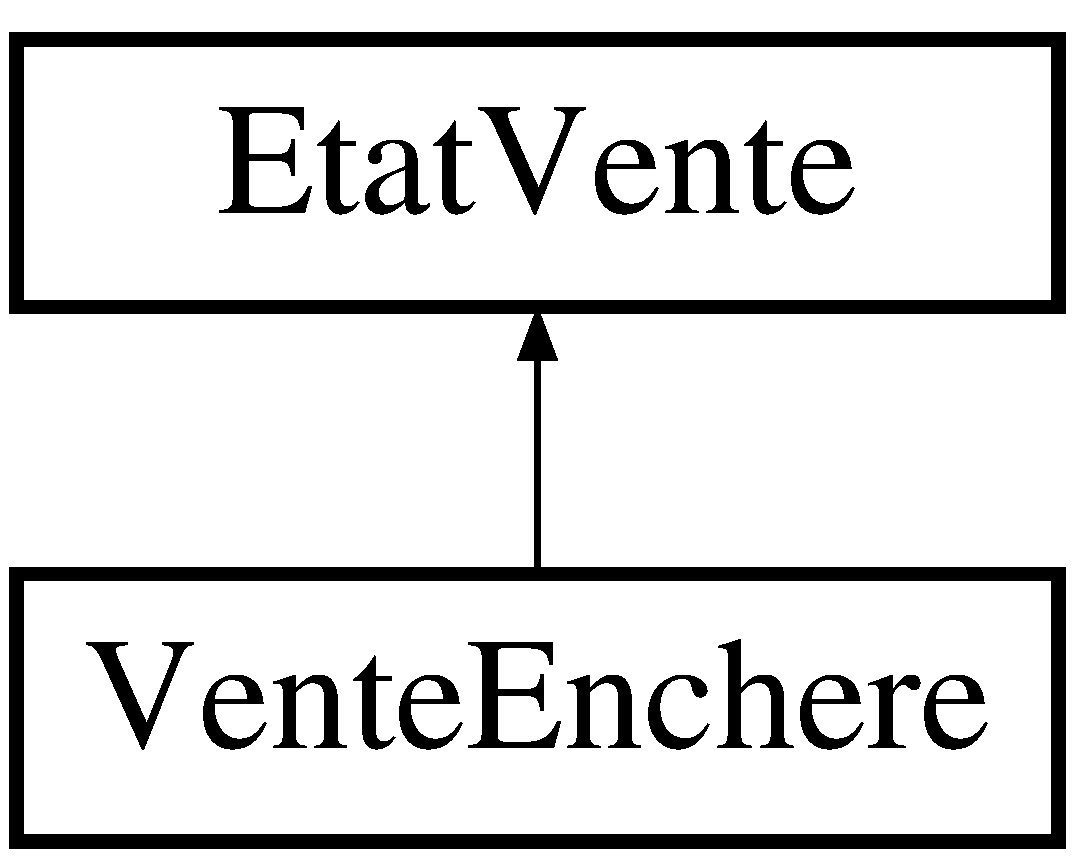
\includegraphics[height=2.000000cm]{class_vente_enchere}
\end{center}
\end{figure}
\subsection*{Fonctions membres publiques}
\begin{DoxyCompactItemize}
\item 
\hyperlink{class_vente_enchere_a383e04cb779ed7a3223b8243a76c13c2}{Vente\-Enchere} (bool b)
\begin{DoxyCompactList}\small\item\em Constructeur de la classe \hyperlink{class_vente_enchere}{Vente\-Enchere}. \end{DoxyCompactList}\item 
\hyperlink{class_vente_enchere_ad2b55c8f2d7cb10f3d124d525c930f9e}{$\sim$\-Vente\-Enchere} ()
\item 
float \hyperlink{class_vente_enchere_a53455121f689127d4daf6123af1668f3}{get\-Prix\-Actuel} ()
\begin{DoxyCompactList}\small\item\em Retourne le prix actuel de la vente. \end{DoxyCompactList}\item 
std\-::string \hyperlink{class_vente_enchere_a2ab7fb32692d9cb1d250b81f0f87dd88}{get\-Date\-Limite} ()
\begin{DoxyCompactList}\small\item\em Retourne la date limite de l'enchère. \end{DoxyCompactList}\item 
void \hyperlink{class_vente_enchere_abad32fe0ea40ea89e1aef1621dc673e6}{set\-Prix\-Actuel} (float prix)
\begin{DoxyCompactList}\small\item\em Cette fonction fixe le prix actuel. \end{DoxyCompactList}\item 
void \hyperlink{class_vente_enchere_a034150f779a519dfc4973a3fcfd0d23e}{set\-Date\-Limite} (struct tm date)
\begin{DoxyCompactList}\small\item\em Cette fonction fixe la date limite. \end{DoxyCompactList}\end{DoxyCompactItemize}
\subsection*{Membres hérités additionnels}


\subsection{Description détaillée}
Cette classe gère une vente aux enchères. 

\subsection{Documentation des constructeurs et destructeur}
\hypertarget{class_vente_enchere_a383e04cb779ed7a3223b8243a76c13c2}{\index{Vente\-Enchere@{Vente\-Enchere}!Vente\-Enchere@{Vente\-Enchere}}
\index{Vente\-Enchere@{Vente\-Enchere}!VenteEnchere@{Vente\-Enchere}}
\subsubsection[{Vente\-Enchere}]{\setlength{\rightskip}{0pt plus 5cm}Vente\-Enchere\-::\-Vente\-Enchere (
\begin{DoxyParamCaption}
\item[{bool}]{b}
\end{DoxyParamCaption}
)}}\label{class_vente_enchere_a383e04cb779ed7a3223b8243a76c13c2}


Constructeur de la classe \hyperlink{class_vente_enchere}{Vente\-Enchere}. 


\begin{DoxyParams}{Paramètres}
{\em b} & -\/ Booléen qui donne le type de la vente \\
\hline
\end{DoxyParams}
\hypertarget{class_vente_enchere_ad2b55c8f2d7cb10f3d124d525c930f9e}{\index{Vente\-Enchere@{Vente\-Enchere}!$\sim$\-Vente\-Enchere@{$\sim$\-Vente\-Enchere}}
\index{$\sim$\-Vente\-Enchere@{$\sim$\-Vente\-Enchere}!VenteEnchere@{Vente\-Enchere}}
\subsubsection[{$\sim$\-Vente\-Enchere}]{\setlength{\rightskip}{0pt plus 5cm}Vente\-Enchere\-::$\sim$\-Vente\-Enchere (
\begin{DoxyParamCaption}
{}
\end{DoxyParamCaption}
)\hspace{0.3cm}{\ttfamily [inline]}}}\label{class_vente_enchere_ad2b55c8f2d7cb10f3d124d525c930f9e}


\subsection{Documentation des fonctions membres}
\hypertarget{class_vente_enchere_a2ab7fb32692d9cb1d250b81f0f87dd88}{\index{Vente\-Enchere@{Vente\-Enchere}!get\-Date\-Limite@{get\-Date\-Limite}}
\index{get\-Date\-Limite@{get\-Date\-Limite}!VenteEnchere@{Vente\-Enchere}}
\subsubsection[{get\-Date\-Limite}]{\setlength{\rightskip}{0pt plus 5cm}std\-::string Vente\-Enchere\-::get\-Date\-Limite (
\begin{DoxyParamCaption}
{}
\end{DoxyParamCaption}
)\hspace{0.3cm}{\ttfamily [virtual]}}}\label{class_vente_enchere_a2ab7fb32692d9cb1d250b81f0f87dd88}


Retourne la date limite de l'enchère. 

\begin{DoxyReturn}{Renvoie}
Un string contenant la date limite de l'enchère 
\end{DoxyReturn}


Réimplémentée à partir de \hyperlink{class_etat_vente_ab466d257671a59ec97ae393c80226b7a}{Etat\-Vente}.

\hypertarget{class_vente_enchere_a53455121f689127d4daf6123af1668f3}{\index{Vente\-Enchere@{Vente\-Enchere}!get\-Prix\-Actuel@{get\-Prix\-Actuel}}
\index{get\-Prix\-Actuel@{get\-Prix\-Actuel}!VenteEnchere@{Vente\-Enchere}}
\subsubsection[{get\-Prix\-Actuel}]{\setlength{\rightskip}{0pt plus 5cm}float Vente\-Enchere\-::get\-Prix\-Actuel (
\begin{DoxyParamCaption}
{}
\end{DoxyParamCaption}
)\hspace{0.3cm}{\ttfamily [virtual]}}}\label{class_vente_enchere_a53455121f689127d4daf6123af1668f3}


Retourne le prix actuel de la vente. 

\begin{DoxyReturn}{Renvoie}
Un float représentant le prix actuel 
\end{DoxyReturn}


Réimplémentée à partir de \hyperlink{class_etat_vente_a0e797a253bbfe990d22f3d2827c8a318}{Etat\-Vente}.

\hypertarget{class_vente_enchere_a034150f779a519dfc4973a3fcfd0d23e}{\index{Vente\-Enchere@{Vente\-Enchere}!set\-Date\-Limite@{set\-Date\-Limite}}
\index{set\-Date\-Limite@{set\-Date\-Limite}!VenteEnchere@{Vente\-Enchere}}
\subsubsection[{set\-Date\-Limite}]{\setlength{\rightskip}{0pt plus 5cm}void Vente\-Enchere\-::set\-Date\-Limite (
\begin{DoxyParamCaption}
\item[{struct tm}]{date}
\end{DoxyParamCaption}
)\hspace{0.3cm}{\ttfamily [virtual]}}}\label{class_vente_enchere_a034150f779a519dfc4973a3fcfd0d23e}


Cette fonction fixe la date limite. 


\begin{DoxyParams}{Paramètres}
{\em date} & -\/ Nouvelle date \\
\hline
\end{DoxyParams}


Réimplémentée à partir de \hyperlink{class_etat_vente_a8efa95982f7252801512df1ea16faeeb}{Etat\-Vente}.

\hypertarget{class_vente_enchere_abad32fe0ea40ea89e1aef1621dc673e6}{\index{Vente\-Enchere@{Vente\-Enchere}!set\-Prix\-Actuel@{set\-Prix\-Actuel}}
\index{set\-Prix\-Actuel@{set\-Prix\-Actuel}!VenteEnchere@{Vente\-Enchere}}
\subsubsection[{set\-Prix\-Actuel}]{\setlength{\rightskip}{0pt plus 5cm}void Vente\-Enchere\-::set\-Prix\-Actuel (
\begin{DoxyParamCaption}
\item[{float}]{prix}
\end{DoxyParamCaption}
)\hspace{0.3cm}{\ttfamily [virtual]}}}\label{class_vente_enchere_abad32fe0ea40ea89e1aef1621dc673e6}


Cette fonction fixe le prix actuel. 


\begin{DoxyParams}{Paramètres}
{\em prix} & -\/ Nouveau prix \\
\hline
\end{DoxyParams}


Réimplémentée à partir de \hyperlink{class_etat_vente_a8436bb978172c8e136fa349706baef0d}{Etat\-Vente}.



La documentation de cette classe a été générée à partir des fichiers suivants \-:\begin{DoxyCompactItemize}
\item 
/home/magalie/\-Bureau/\-S5/\-C\-P\-O\-O\-A/\-Projet/\-E-\/\-Marche-\//iterations/iteration2/\-E\-Marche/bdd/\hyperlink{_vente_enchere_8h}{Vente\-Enchere.\-h}\item 
/home/magalie/\-Bureau/\-S5/\-C\-P\-O\-O\-A/\-Projet/\-E-\/\-Marche-\//iterations/iteration2/\-E\-Marche/bdd/\hyperlink{_vente_enchere_8cpp}{Vente\-Enchere.\-cpp}\end{DoxyCompactItemize}

\hypertarget{class_vente_normale}{\section{Référence de la classe Vente\-Normale}
\label{class_vente_normale}\index{Vente\-Normale@{Vente\-Normale}}
}


Cette classe gère une vente normale.  




{\ttfamily \#include $<$Vente\-Normale.\-h$>$}

Graphe d'héritage de Vente\-Normale\-:\begin{figure}[H]
\begin{center}
\leavevmode
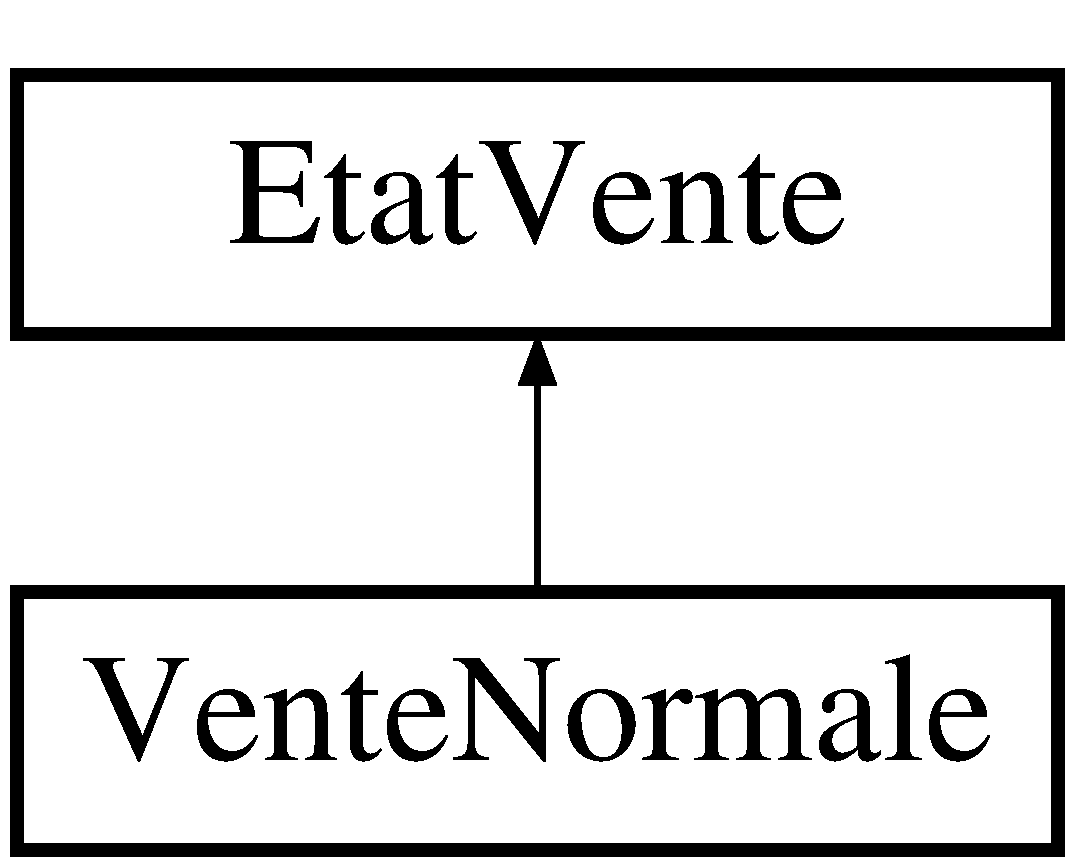
\includegraphics[height=2.000000cm]{class_vente_normale}
\end{center}
\end{figure}
\subsection*{Fonctions membres publiques}
\begin{DoxyCompactItemize}
\item 
\hyperlink{class_vente_normale_a0a419f62780021f774d2039920ea8c86}{Vente\-Normale} (bool b)
\begin{DoxyCompactList}\small\item\em Constructeur de la classe \hyperlink{class_vente_normale}{Vente\-Normale}. \end{DoxyCompactList}\item 
\hyperlink{class_vente_normale_a05bb23b1a3f309cd29bbbb29c09ceed5}{$\sim$\-Vente\-Normale} ()
\end{DoxyCompactItemize}
\subsection*{Membres hérités additionnels}


\subsection{Description détaillée}
Cette classe gère une vente normale. 

\subsection{Documentation des constructeurs et destructeur}
\hypertarget{class_vente_normale_a0a419f62780021f774d2039920ea8c86}{\index{Vente\-Normale@{Vente\-Normale}!Vente\-Normale@{Vente\-Normale}}
\index{Vente\-Normale@{Vente\-Normale}!VenteNormale@{Vente\-Normale}}
\subsubsection[{Vente\-Normale}]{\setlength{\rightskip}{0pt plus 5cm}Vente\-Normale\-::\-Vente\-Normale (
\begin{DoxyParamCaption}
\item[{bool}]{b}
\end{DoxyParamCaption}
)}}\label{class_vente_normale_a0a419f62780021f774d2039920ea8c86}


Constructeur de la classe \hyperlink{class_vente_normale}{Vente\-Normale}. 


\begin{DoxyParams}{Paramètres}
{\em b} & -\/ Booléen qui donne le type de la vente \\
\hline
\end{DoxyParams}
\hypertarget{class_vente_normale_a05bb23b1a3f309cd29bbbb29c09ceed5}{\index{Vente\-Normale@{Vente\-Normale}!$\sim$\-Vente\-Normale@{$\sim$\-Vente\-Normale}}
\index{$\sim$\-Vente\-Normale@{$\sim$\-Vente\-Normale}!VenteNormale@{Vente\-Normale}}
\subsubsection[{$\sim$\-Vente\-Normale}]{\setlength{\rightskip}{0pt plus 5cm}Vente\-Normale\-::$\sim$\-Vente\-Normale (
\begin{DoxyParamCaption}
{}
\end{DoxyParamCaption}
)\hspace{0.3cm}{\ttfamily [inline]}}}\label{class_vente_normale_a05bb23b1a3f309cd29bbbb29c09ceed5}


La documentation de cette classe a été générée à partir des fichiers suivants \-:\begin{DoxyCompactItemize}
\item 
/home/magalie/\-Bureau/\-S5/\-C\-P\-O\-O\-A/\-Projet/\-E-\/\-Marche-\//iterations/itération5/\-E\-Marche/bdd/\hyperlink{_vente_normale_8h}{Vente\-Normale.\-h}\item 
/home/magalie/\-Bureau/\-S5/\-C\-P\-O\-O\-A/\-Projet/\-E-\/\-Marche-\//iterations/itération5/\-E\-Marche/bdd/\hyperlink{_vente_normale_8cpp}{Vente\-Normale.\-cpp}\end{DoxyCompactItemize}

%--- End generated contents ---

% Index
\newpage
\phantomsection
\addcontentsline{toc}{chapter}{Index}
\printindex

\end{document}
